\chapter{All the Pretty Patterns} 
\label{sec:patterns}
\lstset{style=6502Style}

We deserve a rest from reading so much code. So let's take a brief intermission where
we admire all the different patterns that Psychedelia is packaged with. On each of the following
pages we give a 3D rendering of each pattern's evolution according to the
\hyperref[sec:listing_pattern]{\textcolor{blue}{'Sunday Run Algorithm'}}.
On the facing page we provide the two data arrays used to generate the pattern and a step by step
visualisation of the pattern's evolution.

The bad news is that there is some extra code for us to cover from the commercial edition, not much,
but you will find it sprinkled among the pretty pictures and it will hopefully shed some light
on how the commercial edition of Psychedelia managed the large number of patterns available to the
player.

\clearpage
\begin{figure}[H]
    \centering
    \begin{adjustbox}{width=12cm,center}
      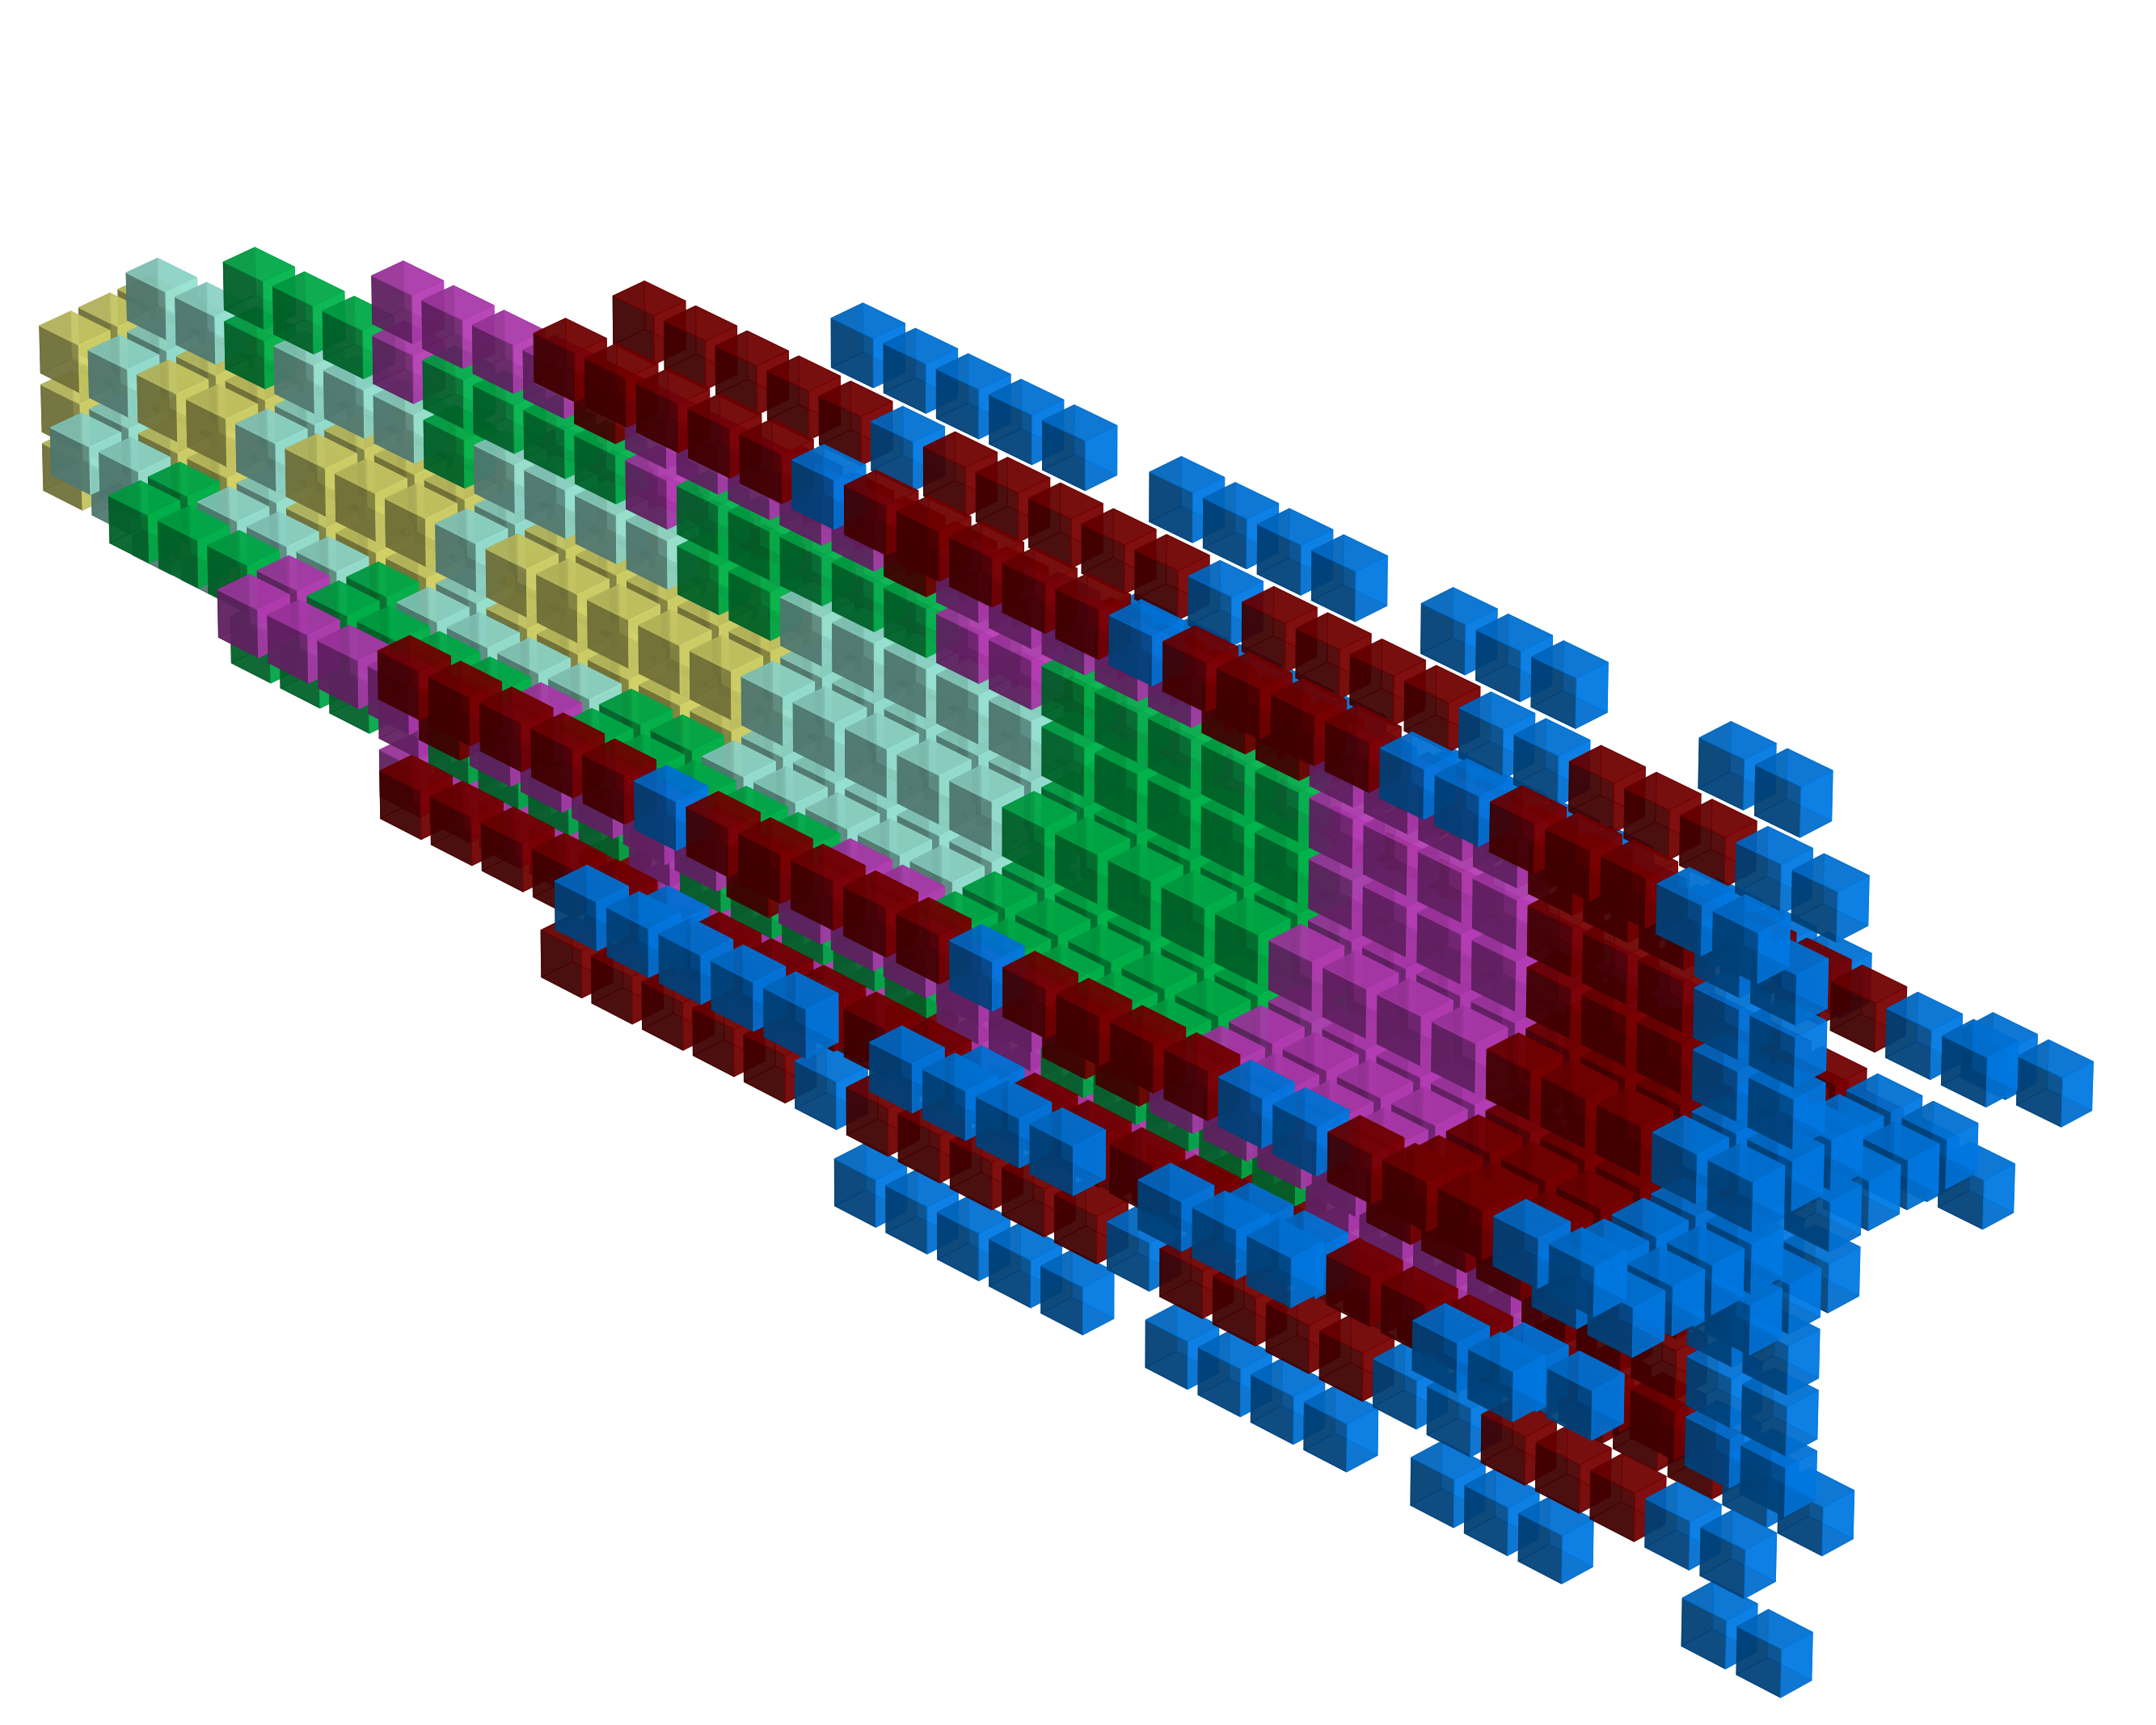
\includegraphics[width=12cm]{src/patterns/pattern0-45.png}%
    \end{adjustbox}
    \begin{adjustbox}{width=12cm,margin=0cm -2cm}
      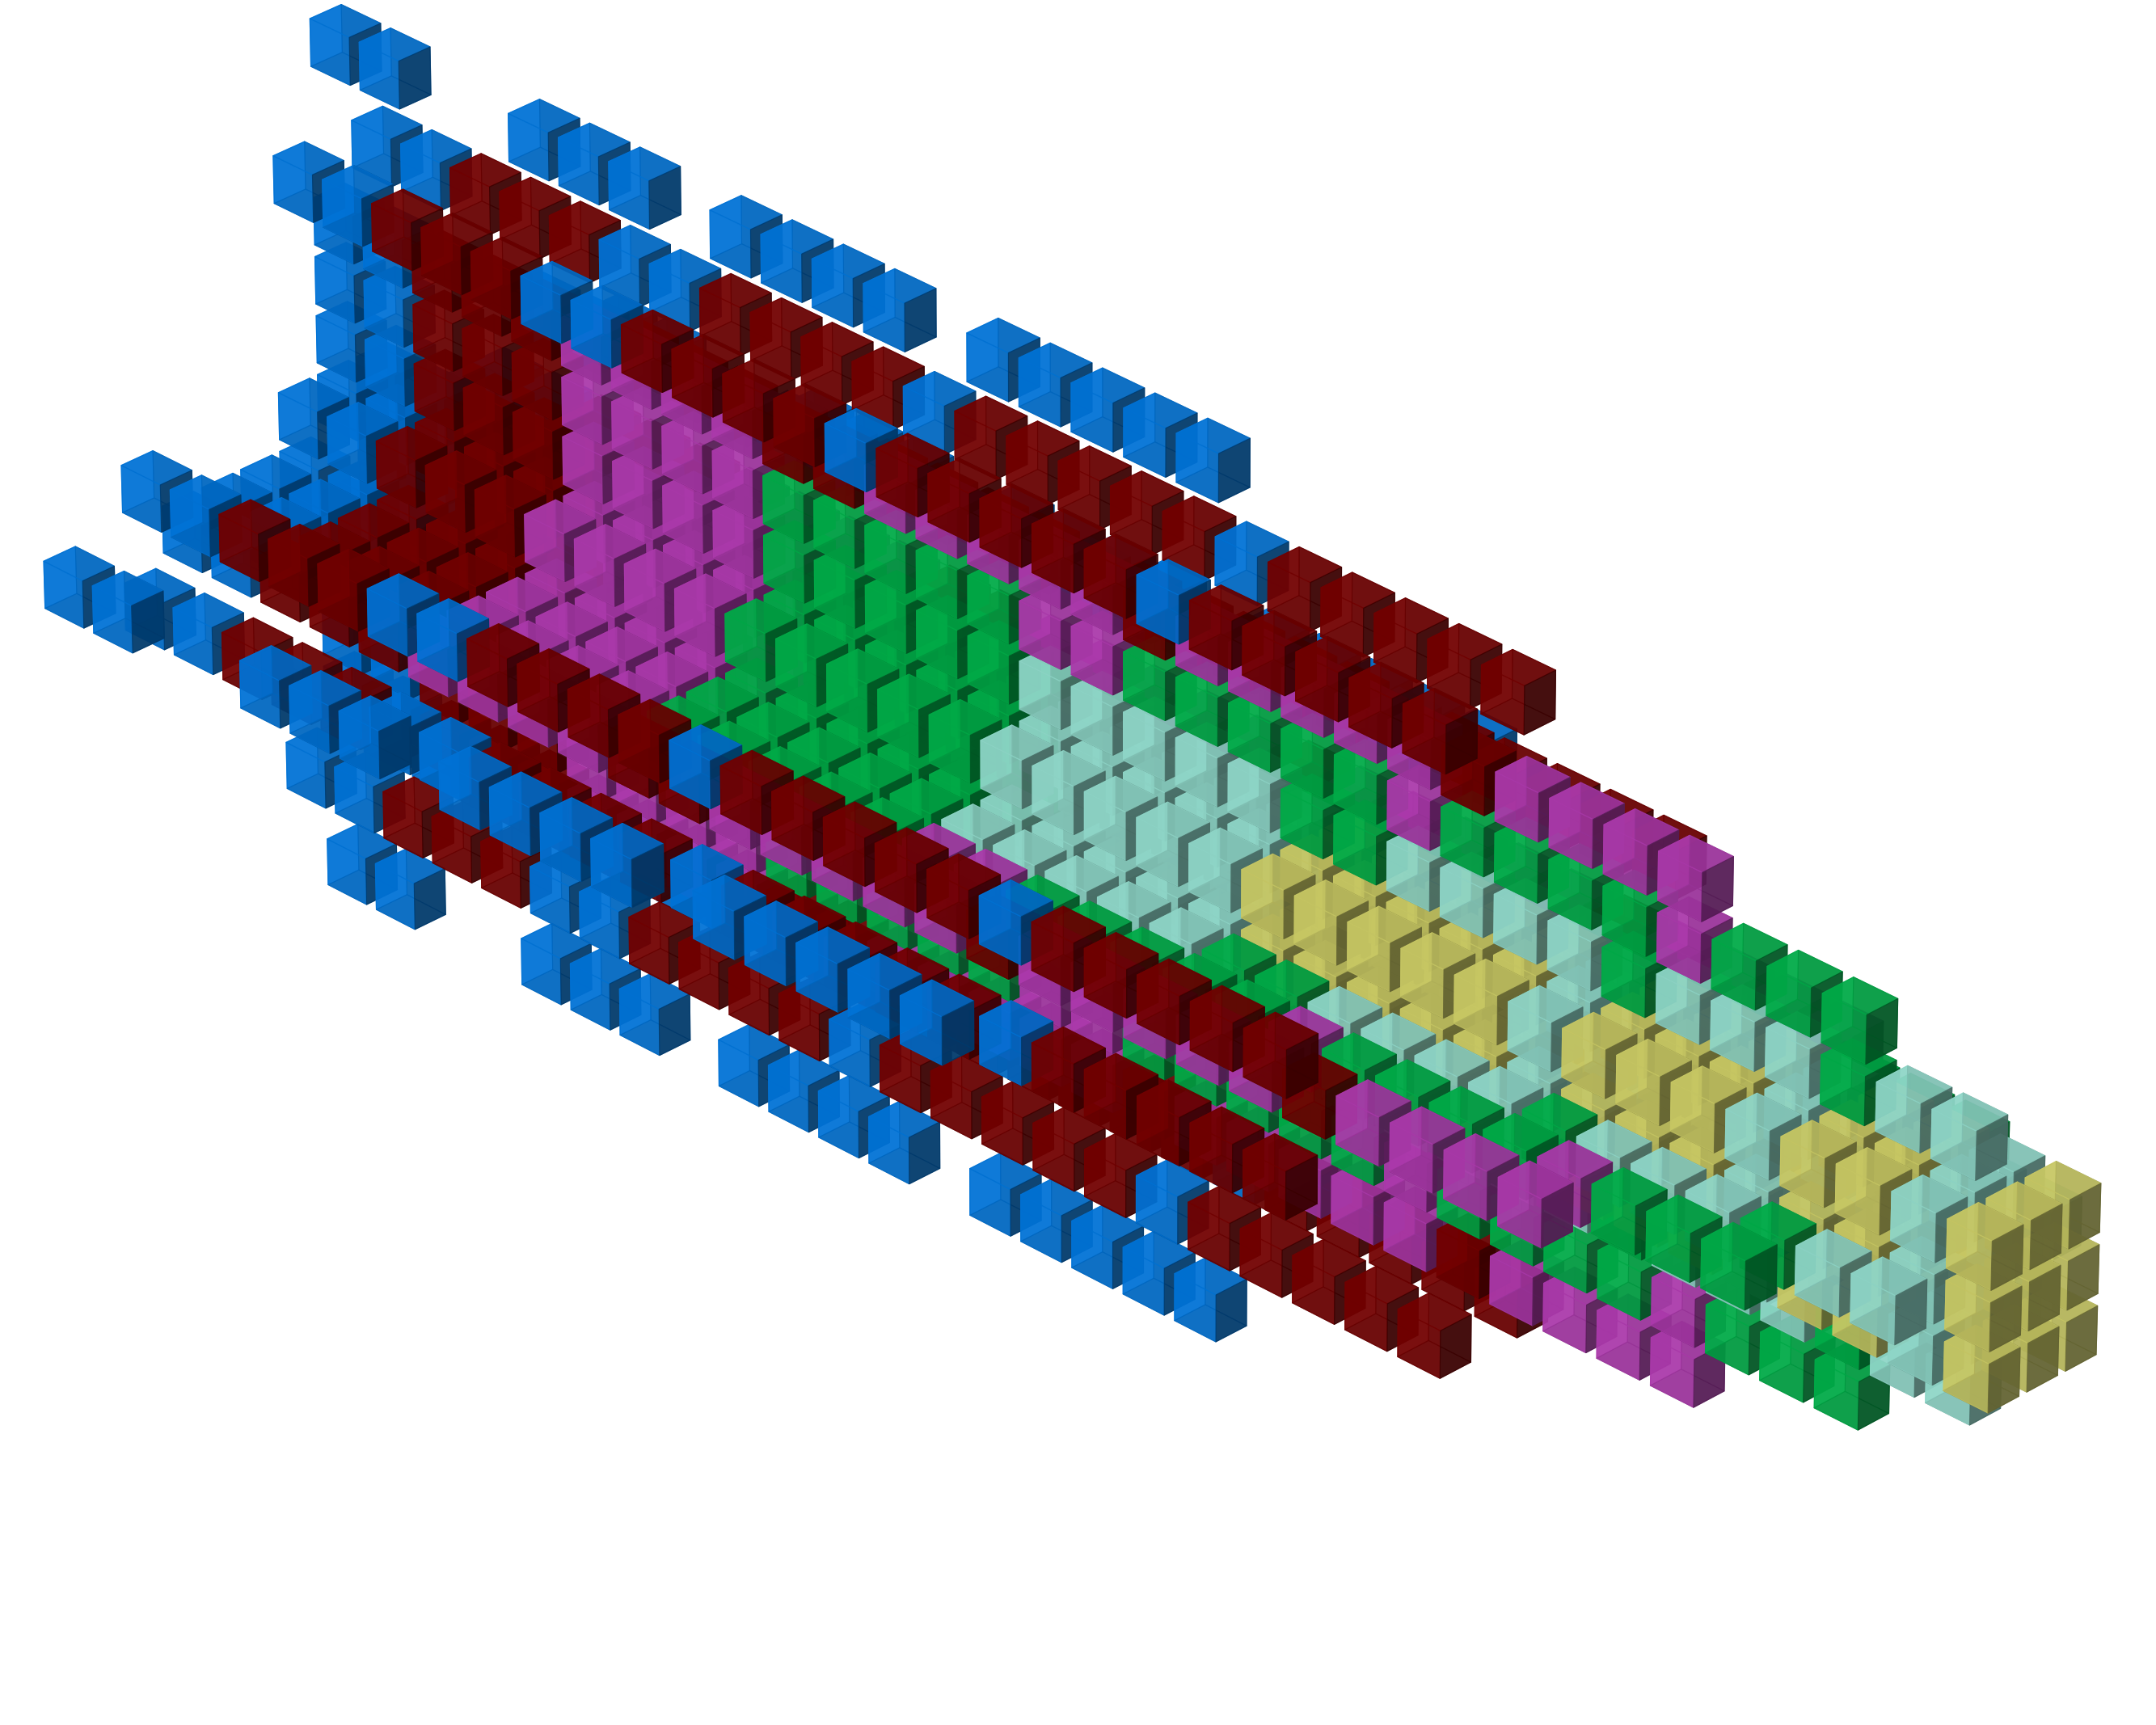
\includegraphics[width=12cm]{src/patterns/pattern0-225.png}%
    \end{adjustbox}
\caption{Evolution of the 'Star One' pattern.}
\end{figure}

\begin{lstlisting}[caption=Source code for the Star.]
starOneXPosArray  
  .BYTE $00,$01,$01,$01,$00,$FF,$FF,$FF,$55       ;        5       
  .BYTE $00,$02,$00,$FE,$55                       ;                
  .BYTE $00,$03,$00,$FD,$55                       ;       4 4      
  .BYTE $00,$04,$00,$FC,$55                       ;        3       
  .BYTE $FF,$01,$05,$05,$01,$FF,$FB,$FB,$55       ;        2       
  .BYTE $00,$07,$00,$F9,$55                       ;        1       
  .BYTE $55                                       ;   4   000   4  
starOneYPosArray                                  ; 5  3210 0123  5  
  .BYTE $FF,$FF,$00,$01,$01,$01,$00,$FF,$55       ;   4   000   4  
  .BYTE $FE,$00,$02,$00,$55                       ;        1       
  .BYTE $FD,$00,$03,$00,$55                       ;        2       
  .BYTE $FC,$00,$04,$00,$55                       ;        3       
  .BYTE $FB,$FB,$FF,$01,$05,$05,$01,$FF,$55       ;       4 4      
  .BYTE $F9,$00,$07,$00,$55                       ;                
  .BYTE $55                                       ;        5       
\end{lstlisting}

\subfile{patterns/tables/pattern0.tex}


\clearpage
\begin{lstlisting}[caption = All the pattern data structures in Psychedelia organized into a set of arrays. 
We use these arrays to choose the correct user-selected pattern at painting time.]
; A pair of arrays together consituting a list of pointers
; to positions in memory containing X position data.
; (i.e. $097C, $0E93,$0EC3, $0F07, $0F23, $0F57, $1161, $11B1)
pixelXPositionLoPtrArray
   .BYTE <starOneXPosArray,<theTwistXPosArray,<laLlamitaXPosArray
   .BYTE <starTwoXPosArray,<deltoidXPosArray,<diffusedXPosArray
   .BYTE <multicrossXPosArray,<pulsarXPosArray
   .BYTE <customPattern0XPosArray,<customPattern1XPosArray
   .BYTE <customPattern2XPosArray,<customPattern3XPosArray
   .BYTE <customPattern4XPosArray,<customPattern5XPosArray
   .BYTE <customPattern6XPosArray,<customPattern7XPosArray

pixelXPositionHiPtrArray 
   .BYTE >starOneXPosArray,>theTwistXPosArray,>laLlamitaXPosArray
   .BYTE >starTwoXPosArray,>deltoidXPosArray,>diffusedXPosArray
   .BYTE >multicrossXPosArray,>pulsarXPosArray
   .BYTE >customPattern0XPosArray,>customPattern1XPosArray
   .BYTE >customPattern2XPosArray,>customPattern3XPosArray
   .BYTE >customPattern4XPosArray,>customPattern5XPosArray
   .BYTE >customPattern6XPosArray,>customPattern7XPosArray


; A pair of arrays together consituting a list of pointers
; to positions in memory containing Y position data.
; (i.e. $097C, $0E93,$0EC3, $0F07, $0F23, $0F57, $1161, $11B1)
pixelYPositionLoPtrArray 
   .BYTE <starOneYPosArray,<theTwistYPosArray,<laLlamitaYPosArray
   .BYTE <starTwoYPosArray,<deltoidYPosArray,<diffusedYPosArray
   .BYTE <multicrossYPosArray,<pulsarYPosArray
   .BYTE <customPattern0YPosArray,<customPattern1YPosArray
   .BYTE <customPattern2YPosArray,<customPattern3YPosArray
   .BYTE <customPattern4YPosArray,<customPattern5YPosArray
   .BYTE <customPattern6YPosArray,<customPattern7YPosArray

pixelYPositionHiPtrArray 
   .BYTE >starOneYPosArray,>theTwistYPosArray,>laLlamitaYPosArray
   .BYTE >starTwoYPosArray,>deltoidYPosArray,>diffusedYPosArray
   .BYTE >multicrossYPosArray,>pulsarYPosArray
   .BYTE >customPattern0YPosArray,>customPattern1YPosArray
   .BYTE >customPattern2YPosArray,>customPattern3YPosArray
   .BYTE >customPattern4YPosArray,>customPattern5YPosArray
   .BYTE >customPattern6YPosArray,>customPattern7YPosArray

\end{lstlisting}
\clearpage

\textbf{Lines 1189-1231. \icode{\textbf{pixelXPositionLoPtrArray/pixelXPositionHiPtrArray}}:} Psychedelia
offers 16 different pretty patterns to choose from, so requires some way of managing them, particularly
when it comes time to painting them on the screen. The four arrays on the opposite page do this job.
They allow us to reference each pattern with an index. For example, index 0 will reference the X and
Y Position data structures for the 'Star One' pattern in \icode{starOneXPosArray} and 
\icode{starOneYPosArray}, index 1 will allow us to reference the data structures for 'The Twist' pattern,
and so on.

On the following pages we'll see how we make practical use of these arrays, but for now we only really
need to make clear that each one contains one byte of the two-byte address at which each
data structure is stored. The use of \icode{<} and \icode{>} in the listing is a convention that
tells the assembler we're looking at the first byte (\icode{>}) or the second byte (\icode{<}).
Hopefully this table makes this explicit to the reader:

\begin{figure}[H]
  {
    \setlength{\tabcolsep}{3.0pt}
    \setlength\cmidrulewidth{\heavyrulewidth} % Make cmidrule = 
    \begin{adjustbox}{width=8cm,center}
      \begin{tabular}{ccccc}
        \toprule
        Element &
        \makecell[c]{\icode{pixelXPosition} \\ \icode{HiPtrArray}} & 
        \makecell[c]{\icode{pixelXPosition} \\ \icode{LoPtrArray}} & 
        Address &
        Name \\
        \midrule
        0 & \icode{\$09} & \icode{\$7C} & \icode{\$097C} & \icode{starOneXPosArray} \\ 
        1 & \icode{\$0E} & \icode{\$93} & \icode{\$0E93}  & \icode{theTwistXPosArray}\\ 
        2 & \icode{\$0E} & \icode{\$C3} & \icode{\$0EC3}  & \icode{laLlamitaXPosArray}\\ 
        3 & \icode{\$0F} & \icode{\$07} & \icode{\$0F07}  & \icode{starTwoXPosArray}\\ 
        4 & \icode{\$0F} & \icode{\$23} & \icode{\$0F23}  & \icode{deltoidXPosArray}\\ 
        5 & \icode{\$0F} & \icode{\$57} & \icode{\$0F57}  & \icode{diffusedXPosArray}\\ 
        . & . & . & . &. \\
        15 & \icode{\$CE} & \icode{\$00} & \icode{\$CE00}  & \icode{customPattern6XPosArray}\\ 
        16 & \icode{\$CF} & \icode{\$00} & \icode{\$CF00}  & \icode{customPattern7XPosArray}\\ 
        \bottomrule
      \end{tabular}
    \end{adjustbox}
  }\caption{Our two arrays and their contents - each combining to give us an address for the X
  Position data structure for each pattern. The line with ellipses indicates that we've left out some elements for the
  sake of brevity.}
\end{figure}
\vspace*{-\baselineskip}

\textbf{Lines 1189-1231. \icode{\textbf{pixelYPositionLoPtrArray/pixelYPositionHiPtrArray}}:} As for the X position array,
so for the Y position array. 
\begin{figure}[H]
  {
    \setlength{\tabcolsep}{3.0pt}
    \setlength\cmidrulewidth{\heavyrulewidth} % Make cmidrule = 
    \begin{adjustbox}{width=8cm,center}
      \begin{tabular}{ccccc}
        \toprule
        Element &
        \makecell[c]{\icode{pixelYPosition} \\ \icode{HiPtrArray}} & 
        \makecell[c]{\icode{pixelYPosition} \\ \icode{LoPtrArray}} & 
        Address &
        Name \\
        \midrule
        0 & \icode{\$09} & \icode{\$A3} & \icode{\$09A3} & \icode{starOneYPosArray} \\ 
        1 & \icode{\$0E} & \icode{\$AB} & \icode{\$0EAB}  & \icode{theTwistYPosArray}\\ 
        2 & \icode{\$0E} & \icode{\$E5} & \icode{\$0EE5}  & \icode{laLlamitaYPosArray}\\ 
        . & . & . & . &. \\
        15 & \icode{\$CE} & \icode{\$00} & \icode{\$CE00}  & \icode{customPattern6YPosArray}\\ 
        16 & \icode{\$CF} & \icode{\$00} & \icode{\$CF00}  & \icode{customPattern7YPosArray}\\ 
        \bottomrule
      \end{tabular}
    \end{adjustbox}
  }\caption{Our two arrays and their contents - each combining to give us an address for the Y
  Position data structure for each pattern. }
\end{figure}
\clearpage
\begin{figure}[H]
    \centering
    \begin{adjustbox}{width=12cm,center}
      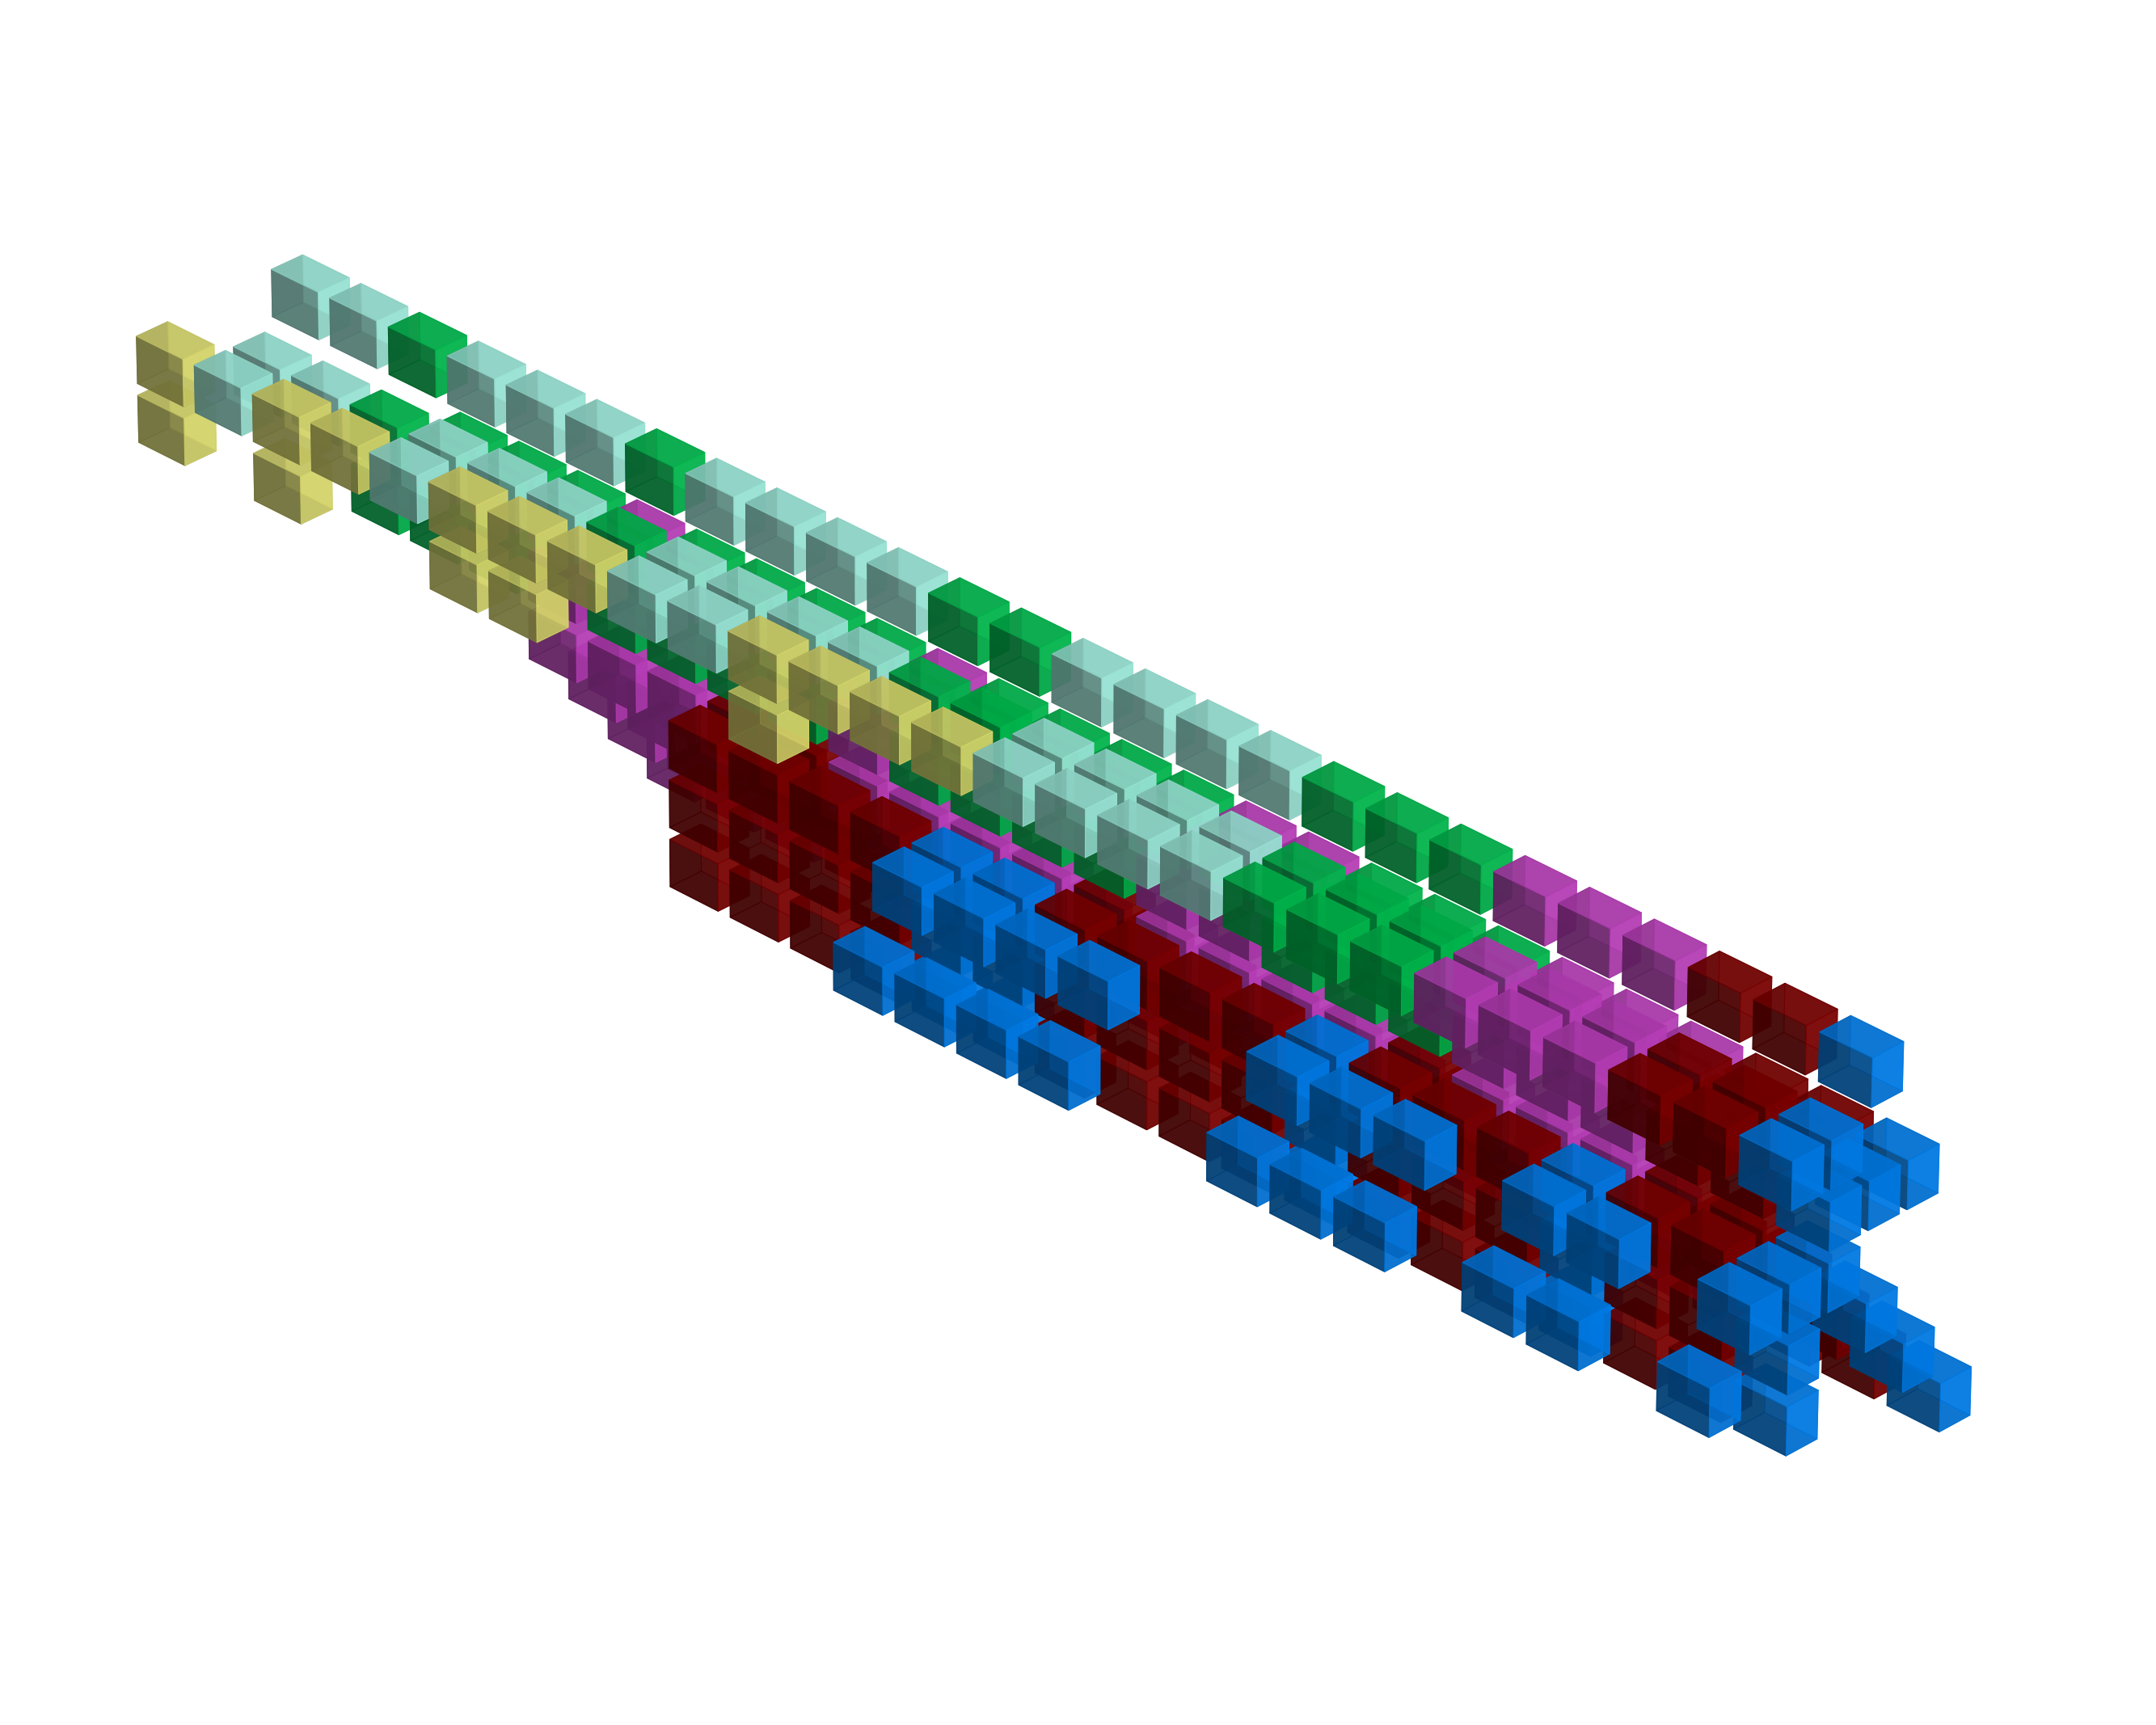
\includegraphics[width=12cm]{src/patterns/pattern1-45.png}%
    \end{adjustbox}
    \begin{adjustbox}{width=12cm,margin=0cm -4cm}
      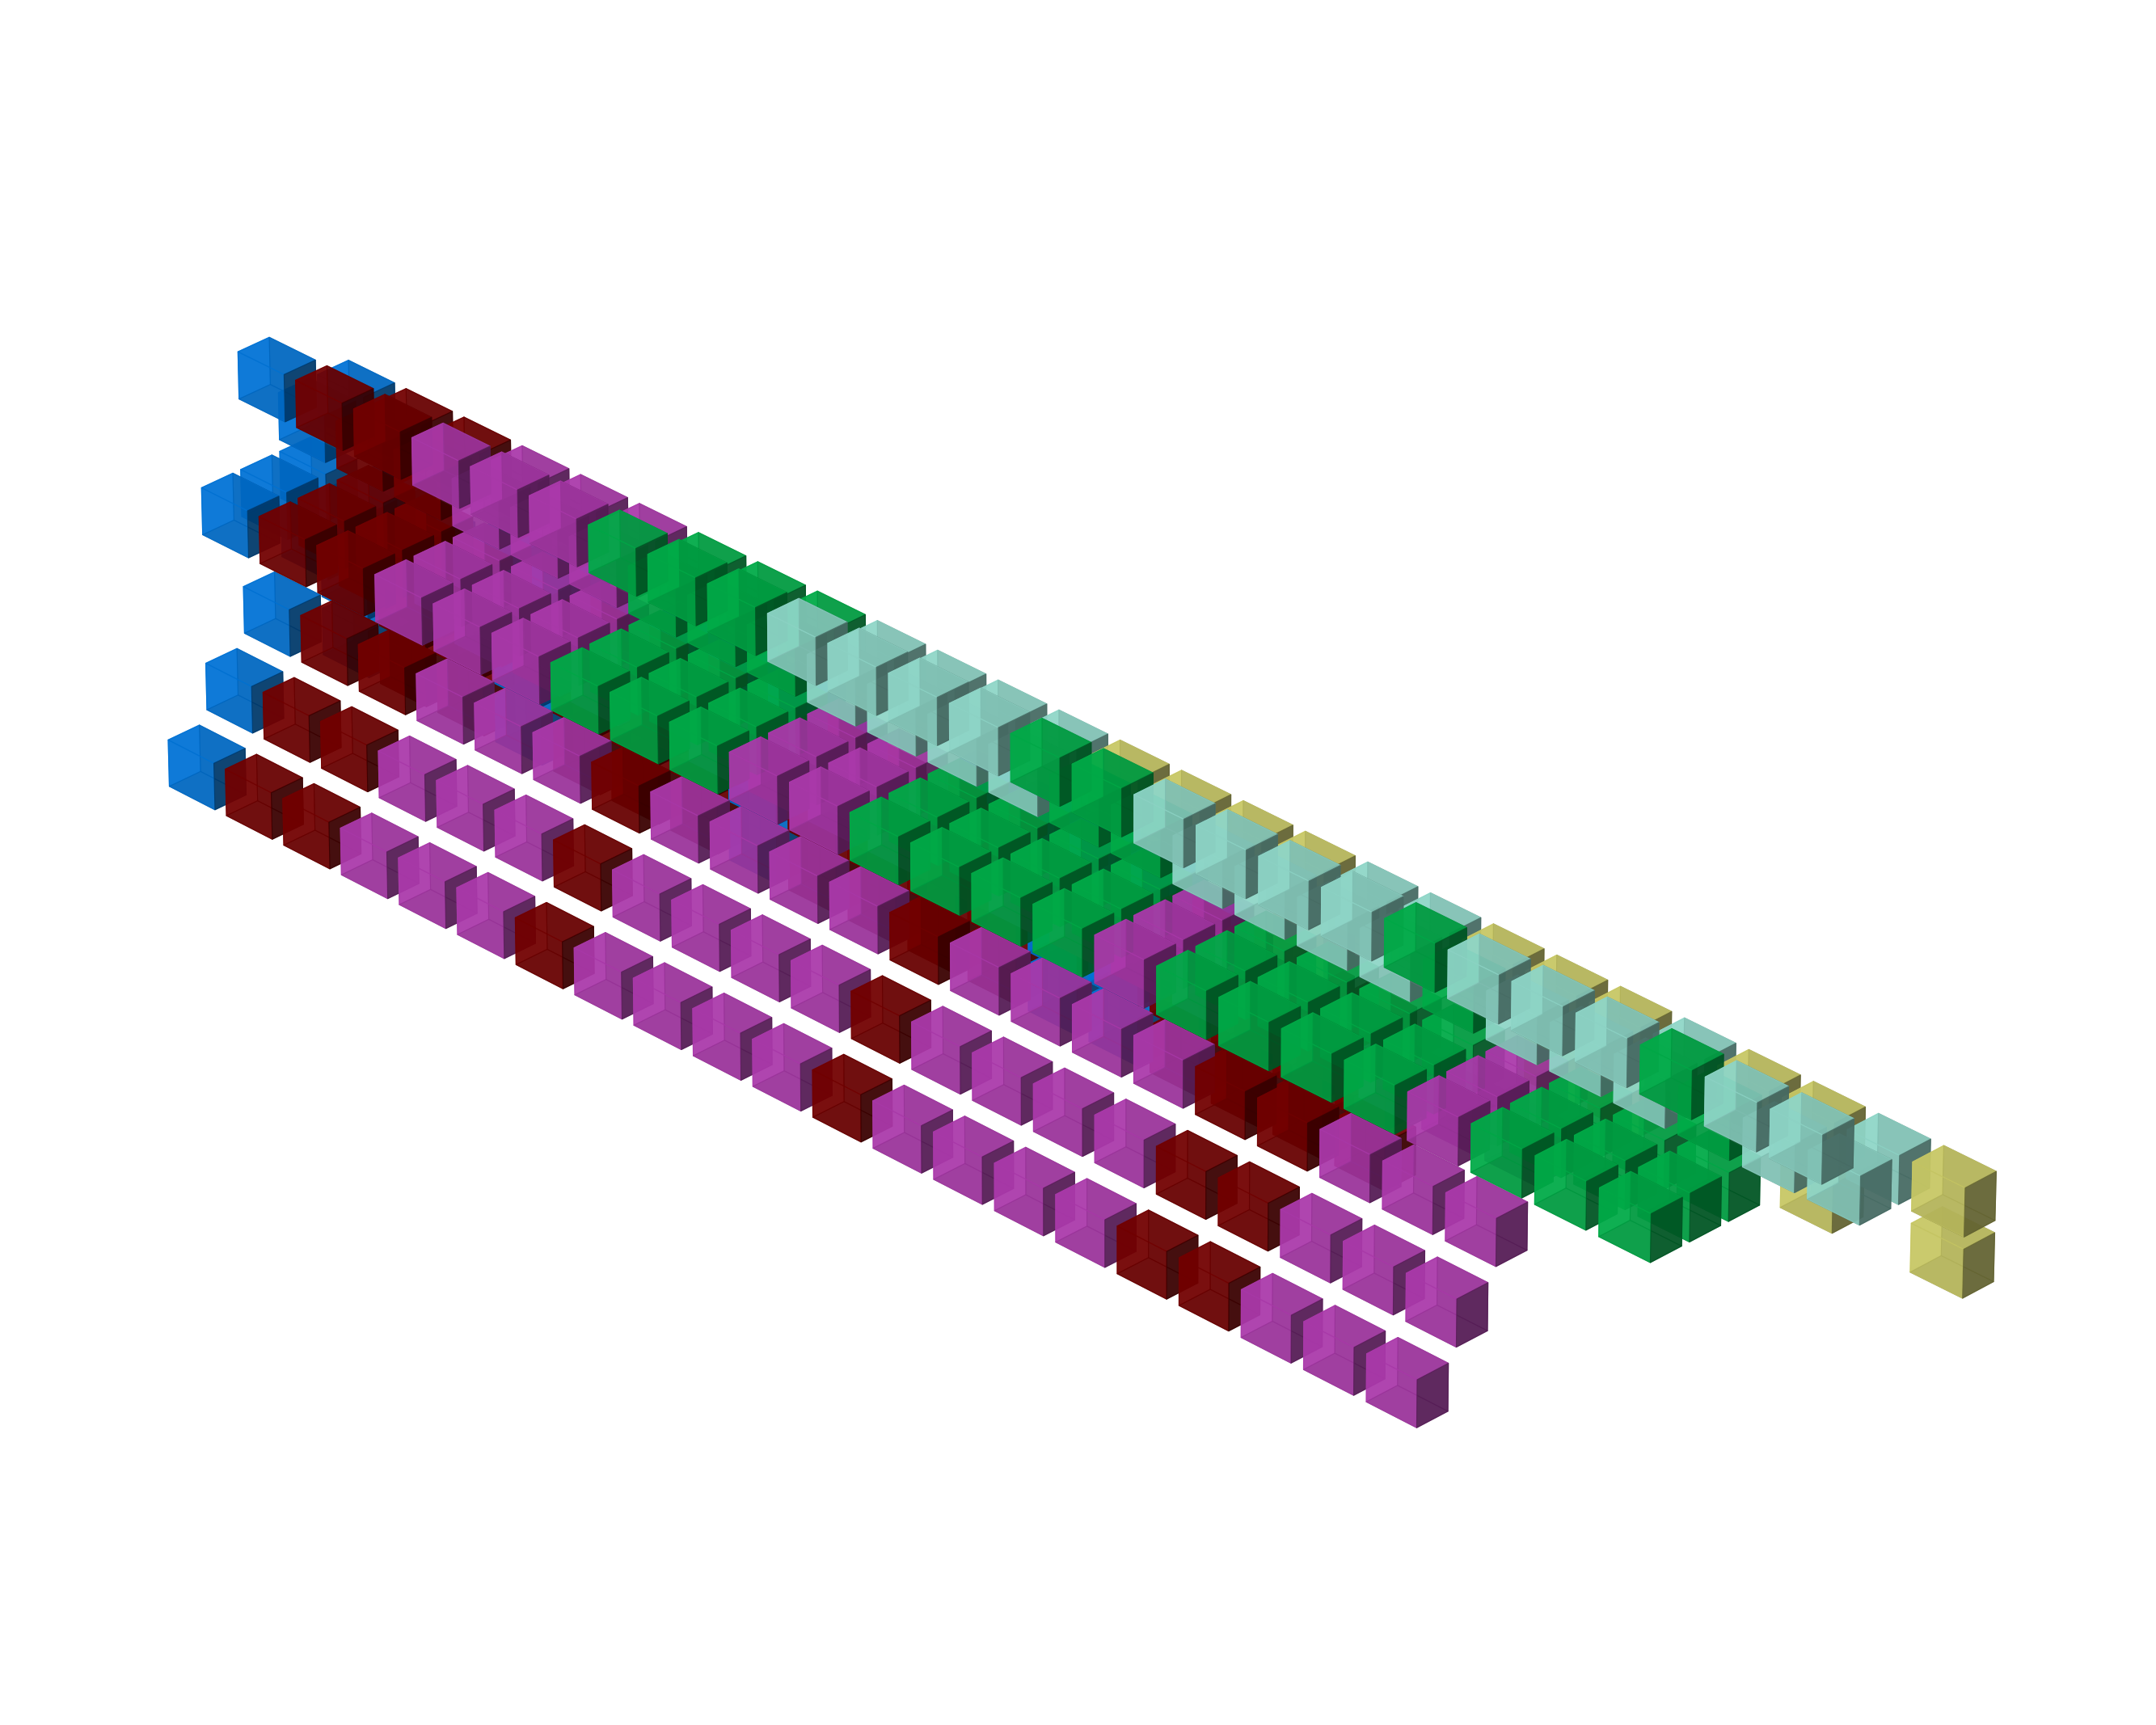
\includegraphics[width=12cm]{src/patterns/pattern1-225.png}%
    \end{adjustbox}
\caption{The 'Twist'.}
\end{figure}
\clearpage

\begin{lstlisting}
theTwistXPosArray .BYTE $00,$55                            ;     1  
                  .BYTE $01,$02,$55                        ;   01   
                  .BYTE $01,$02,$03,$55                    ;  6 222 
                  .BYTE $01,$02,$03,$04,$55                ;  543   
                  .BYTE $00,$00,$00,$55                    ; 5 4 3  
                  .BYTE $FF,$FE,$55                        ;   4  3 
                  .BYTE $FF,$55                            ;       3
                  .BYTE $55
theTwistYPosArray .BYTE $FF,$55
                  .BYTE $FF,$FE,$55
                  .BYTE $00,$00,$00,$55
                  .BYTE $01,$02,$03,$04,$55
                  .BYTE $01,$02,$03,$55
                  .BYTE $01,$02,$55
                  .BYTE $00,$55
                  .BYTE $55
\end{lstlisting}
\subfile{patterns/tables/pattern1.tex}

\clearpage
\begin{lstlisting}[basicstyle=\ttfamily\scriptsize, caption=The routine responsible for painting patterns.]
xPosLoPtr = $0D
xPosHiPtr = $0E
yPosLoPtr = $10
yPosHiPtr = $11
;-------------------------------------------------------
; PaintStructureAtCurrentPosition
;-------------------------------------------------------
PaintStructureAtCurrentPosition   
        JSR PaintPixelForCurrentSymmetry
        LDY #$00
        LDA baseLevelForCurrentPixel
        CMP #$07
        BNE CanLoopAndPaint
        RTS 

CanLoopAndPaint   
        LDA #$07
        STA countToMatchCurrentIndex

        LDA pixelXPosition
        STA previousCursorXPosition
        LDA pixelYPosition
        STA previousPixelYPosition

        LDX patternIndex
        LDA pixelXPositionLoPtrArray,X
        STA xPosLoPtr
        LDA pixelXPositionHiPtrArray,X
        STA xPosHiPtr
        LDA pixelYPositionLoPtrArray,X
        STA yPosLoPtr
        LDA pixelYPositionHiPtrArray,X
        STA yPosHiPtr

        ; Paint pixels in the sequence until hitting a break
        ; at $55
PixelPaintLoop   
        ; Get the next byte from the pattern's X pos array.
        LDA previousCursorXPosition
        CLC 
        ADC (xPosLoPtr),Y
        STA pixelXPosition

        ; Get the next byte from the pattern's Y pos array.
        LDA previousPixelYPosition
        CLC 
        ADC (yPosLoPtr),Y
        STA pixelYPosition

        ; Push Y to the stack.
        TYA 
        PHA 

        JSR PaintPixelForCurrentSymmetry

        ; Pull Y back from the stack and increment
        PLA 
        TAY 
        INY 
\end{lstlisting}
\clearpage

\textbf{Lines 1189-1231. \icode{\textbf{PaintStructureAtCurrentPosition}}:} We've already encountered this routine
in \hyperref[sec:listing_commentary]{\textcolor{blue}{ our walk through of the listing.}}. This is the version that shipped 
with the commercial edition of Psychedelia so has a necessary extra complication to deal with the fact that we 
are going to paint one of up to 16 possible patterns. What we want to figure out here is the X and Y position we should
paint for each element in the pattern's data structure.

The pattern the user has selected is stored as an index value in \icode{patternIndex}. We use it to fetch the element
from each array:
\begin{lstlisting}[basicstyle=\ttfamily\scriptsize]
        LDX patternIndex
        LDA pixelXPositionLoPtrArray,X
        STA xPosLoPtr
        LDA pixelXPositionHiPtrArray,X
        STA xPosHiPtr
        LDA pixelYPositionLoPtrArray,X
        STA yPosLoPtr
        LDA pixelYPositionHiPtrArray,X
        STA yPosHiPtr
\end{lstlisting}

Imagine our \icode{patternIndex} is \icode{1}. This will give us the following values: 

\begin{figure}[H]
  {
    \setlength{\tabcolsep}{3.0pt}
    \setlength\cmidrulewidth{\heavyrulewidth} % Make cmidrule = 
    \begin{adjustbox}{width=7cm,center}
      \begin{tabular}{cccc}
        \toprule
        \icode{xPosHiPtr} &
        \icode{xPosLoPtr} &
        Address &
        Name \\
        \midrule
        \icode{\$0E} & \icode{\$93} & \icode{\$0E93}  & \icode{theTwistXPosArray}\\ 
        \bottomrule
      \end{tabular}
    \end{adjustbox}
  }
\end{figure}
\vspace*{-\baselineskip}

Now, using this as our basis we can read each byte from this address onwards (from each array) and
use it to calculate the X and Y position to paint a pixel at. Recall that the way we read the 
\icode{theTwistXPosArray} and \icode{theTwistYPosArray} data structures is to treat each element
as an offset from the cursor's current X/Y position. So that means taking \icode{previousCursorXPosition}
and adding the value we read from the array  to it. The way we read in a byte from the array using \icode{xPosLoPtr}
and add it to get the new position is as follows:

\begin{lstlisting}[basicstyle=\ttfamily\scriptsize]
        LDA previousCursorXPosition
        CLC 
        ADC (xPosLoPtr),Y
        STA pixelXPosition
\end{lstlisting}

\icode{(xPosLoPtr)} in the above does something very useful: it points to the address you get from combining
\icode{xPosLoPtr} \icode{(\$93)} and \icode{xPosHiPtr} \icode{(\$0E)}. It can do this because \icode{xPosLoPtr}
and \icode{xPosHiPtr} are adjacent to each other in memory.

With \icode{Y} as an offset  (Y is the counter in our loop,
incremented at each iteration) \icode{ADC} is able to point to the next byte in the \icode{theTwistXPosArray} and add it to
the accumulator, so that we can store our result in \icode{pixelXPosition}.
 
\clearpage
\begin{figure}[H]
    \centering
    \begin{adjustbox}{width=12cm,center}
      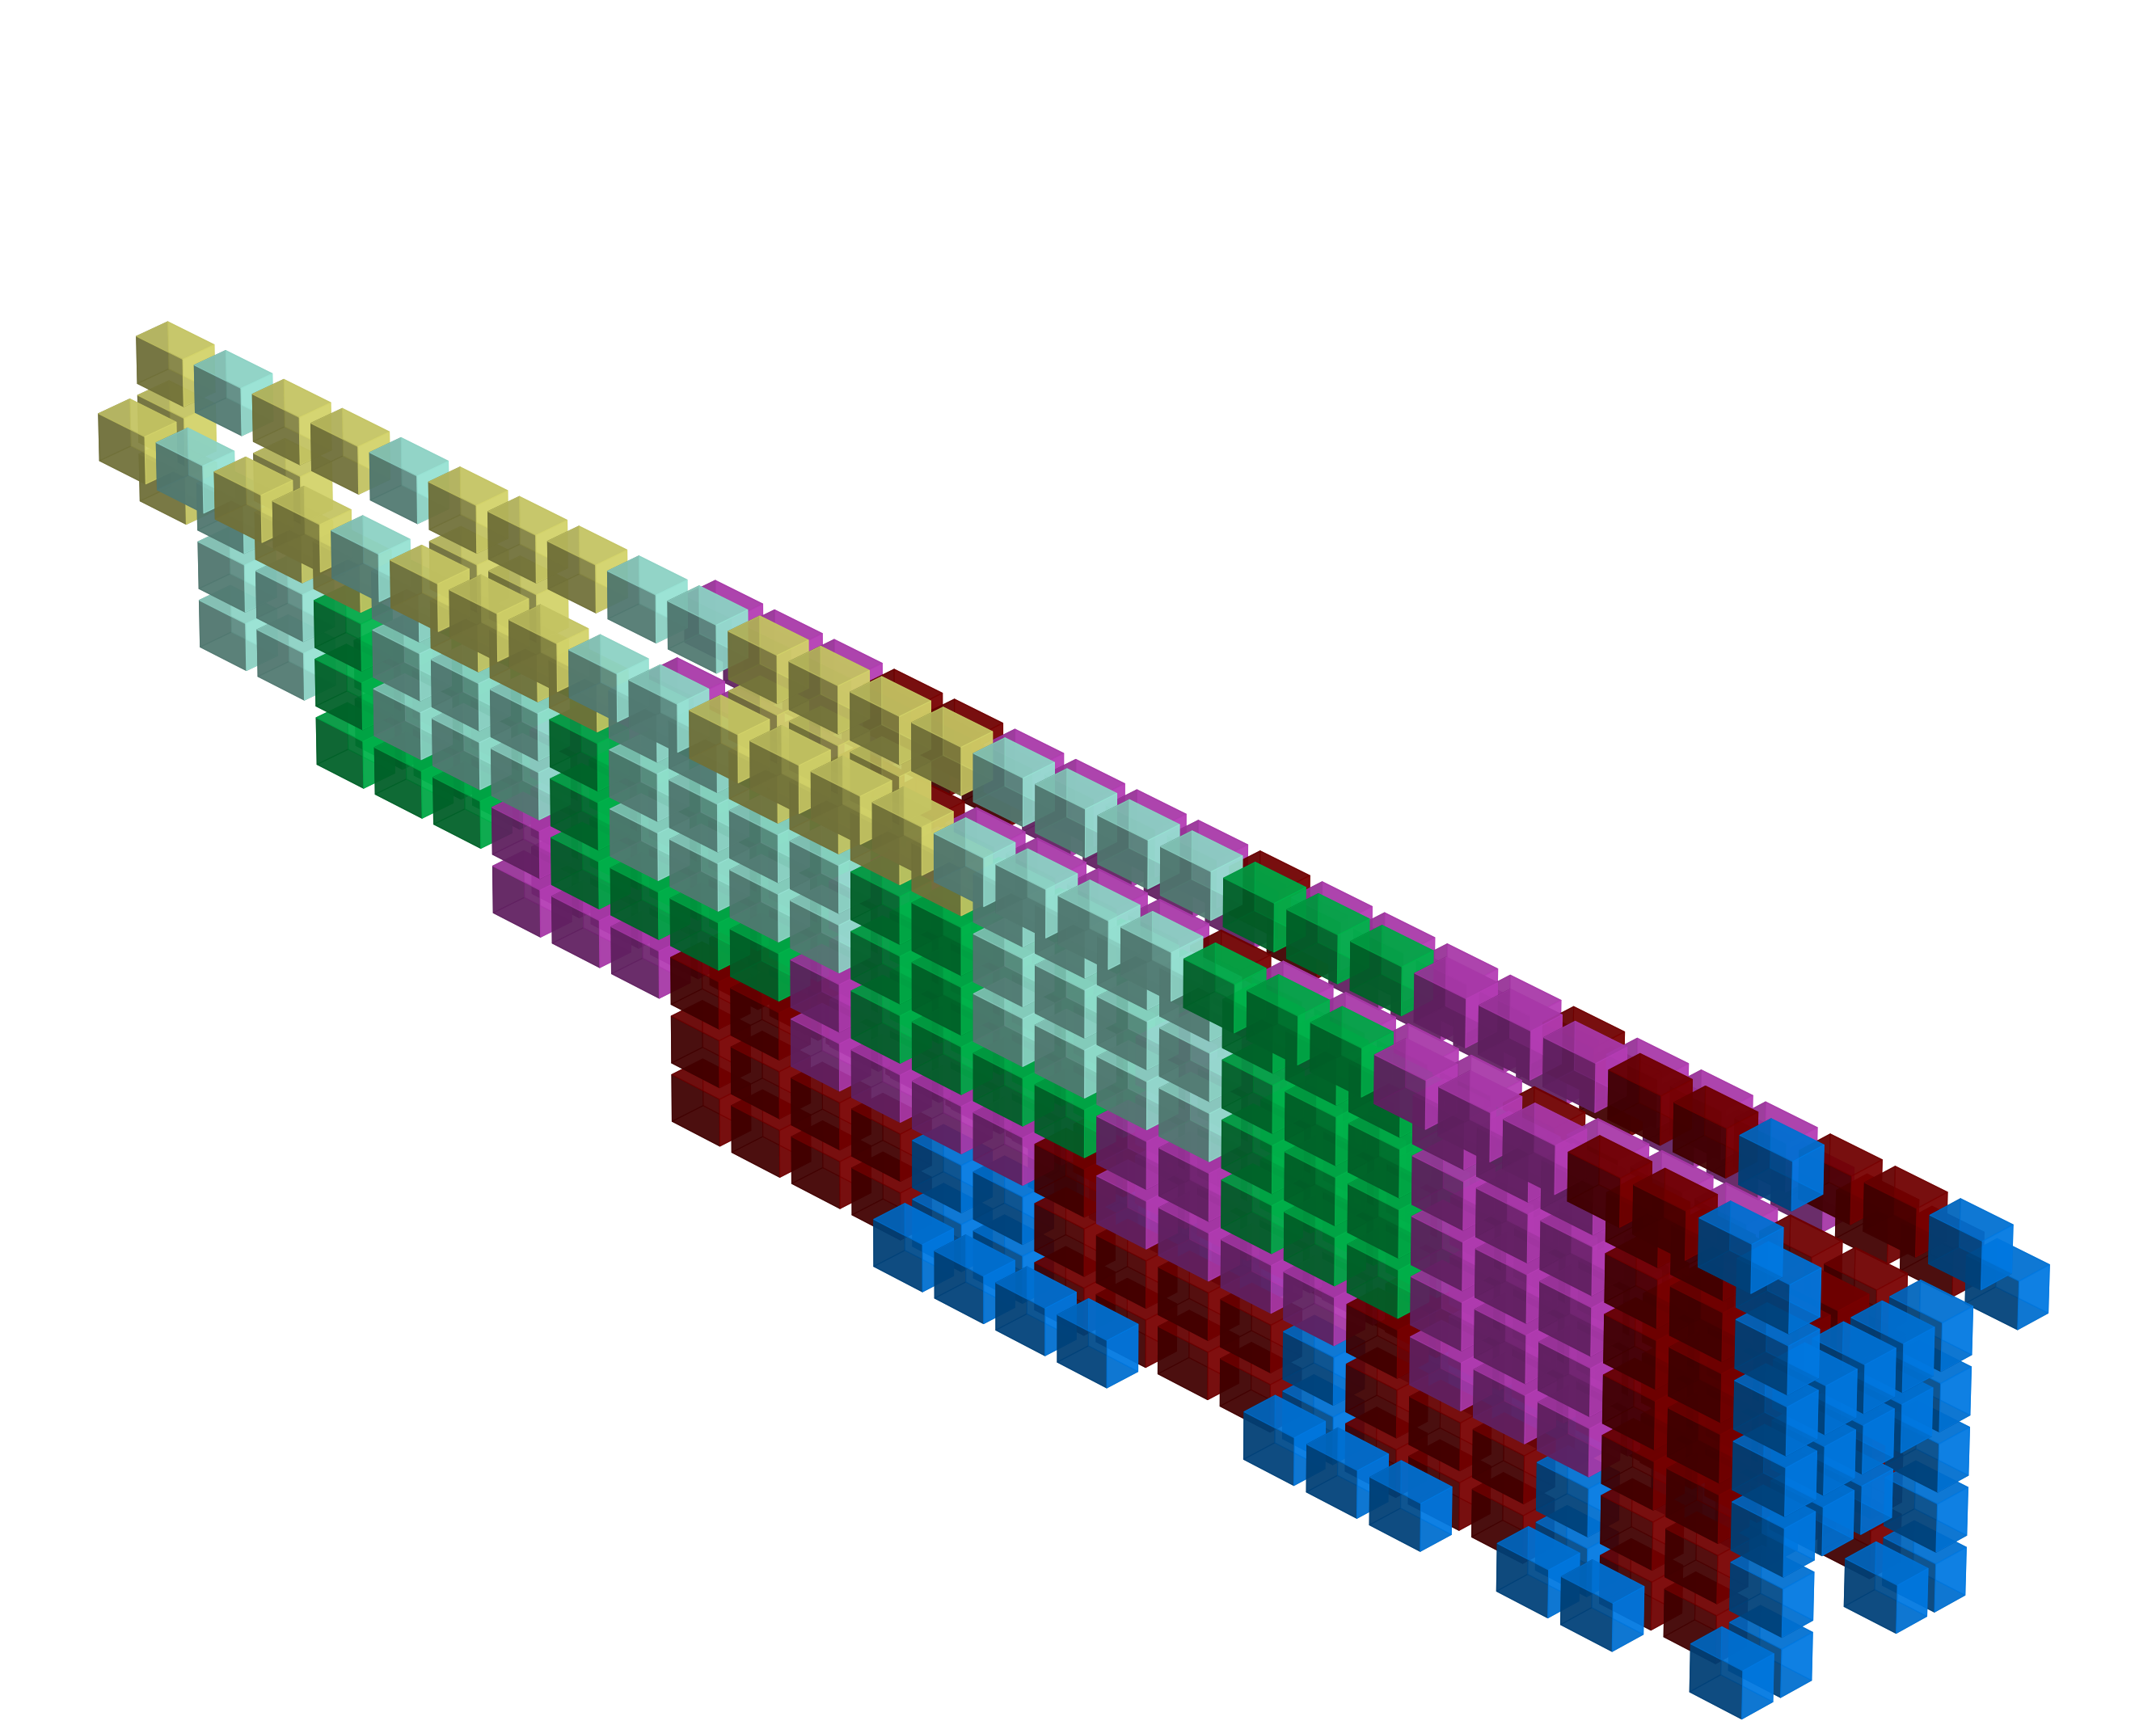
\includegraphics[width=12cm]{src/patterns/pattern2-45.png}%
    \end{adjustbox}
    \begin{adjustbox}{width=12cm,margin=0cm -4cm}
      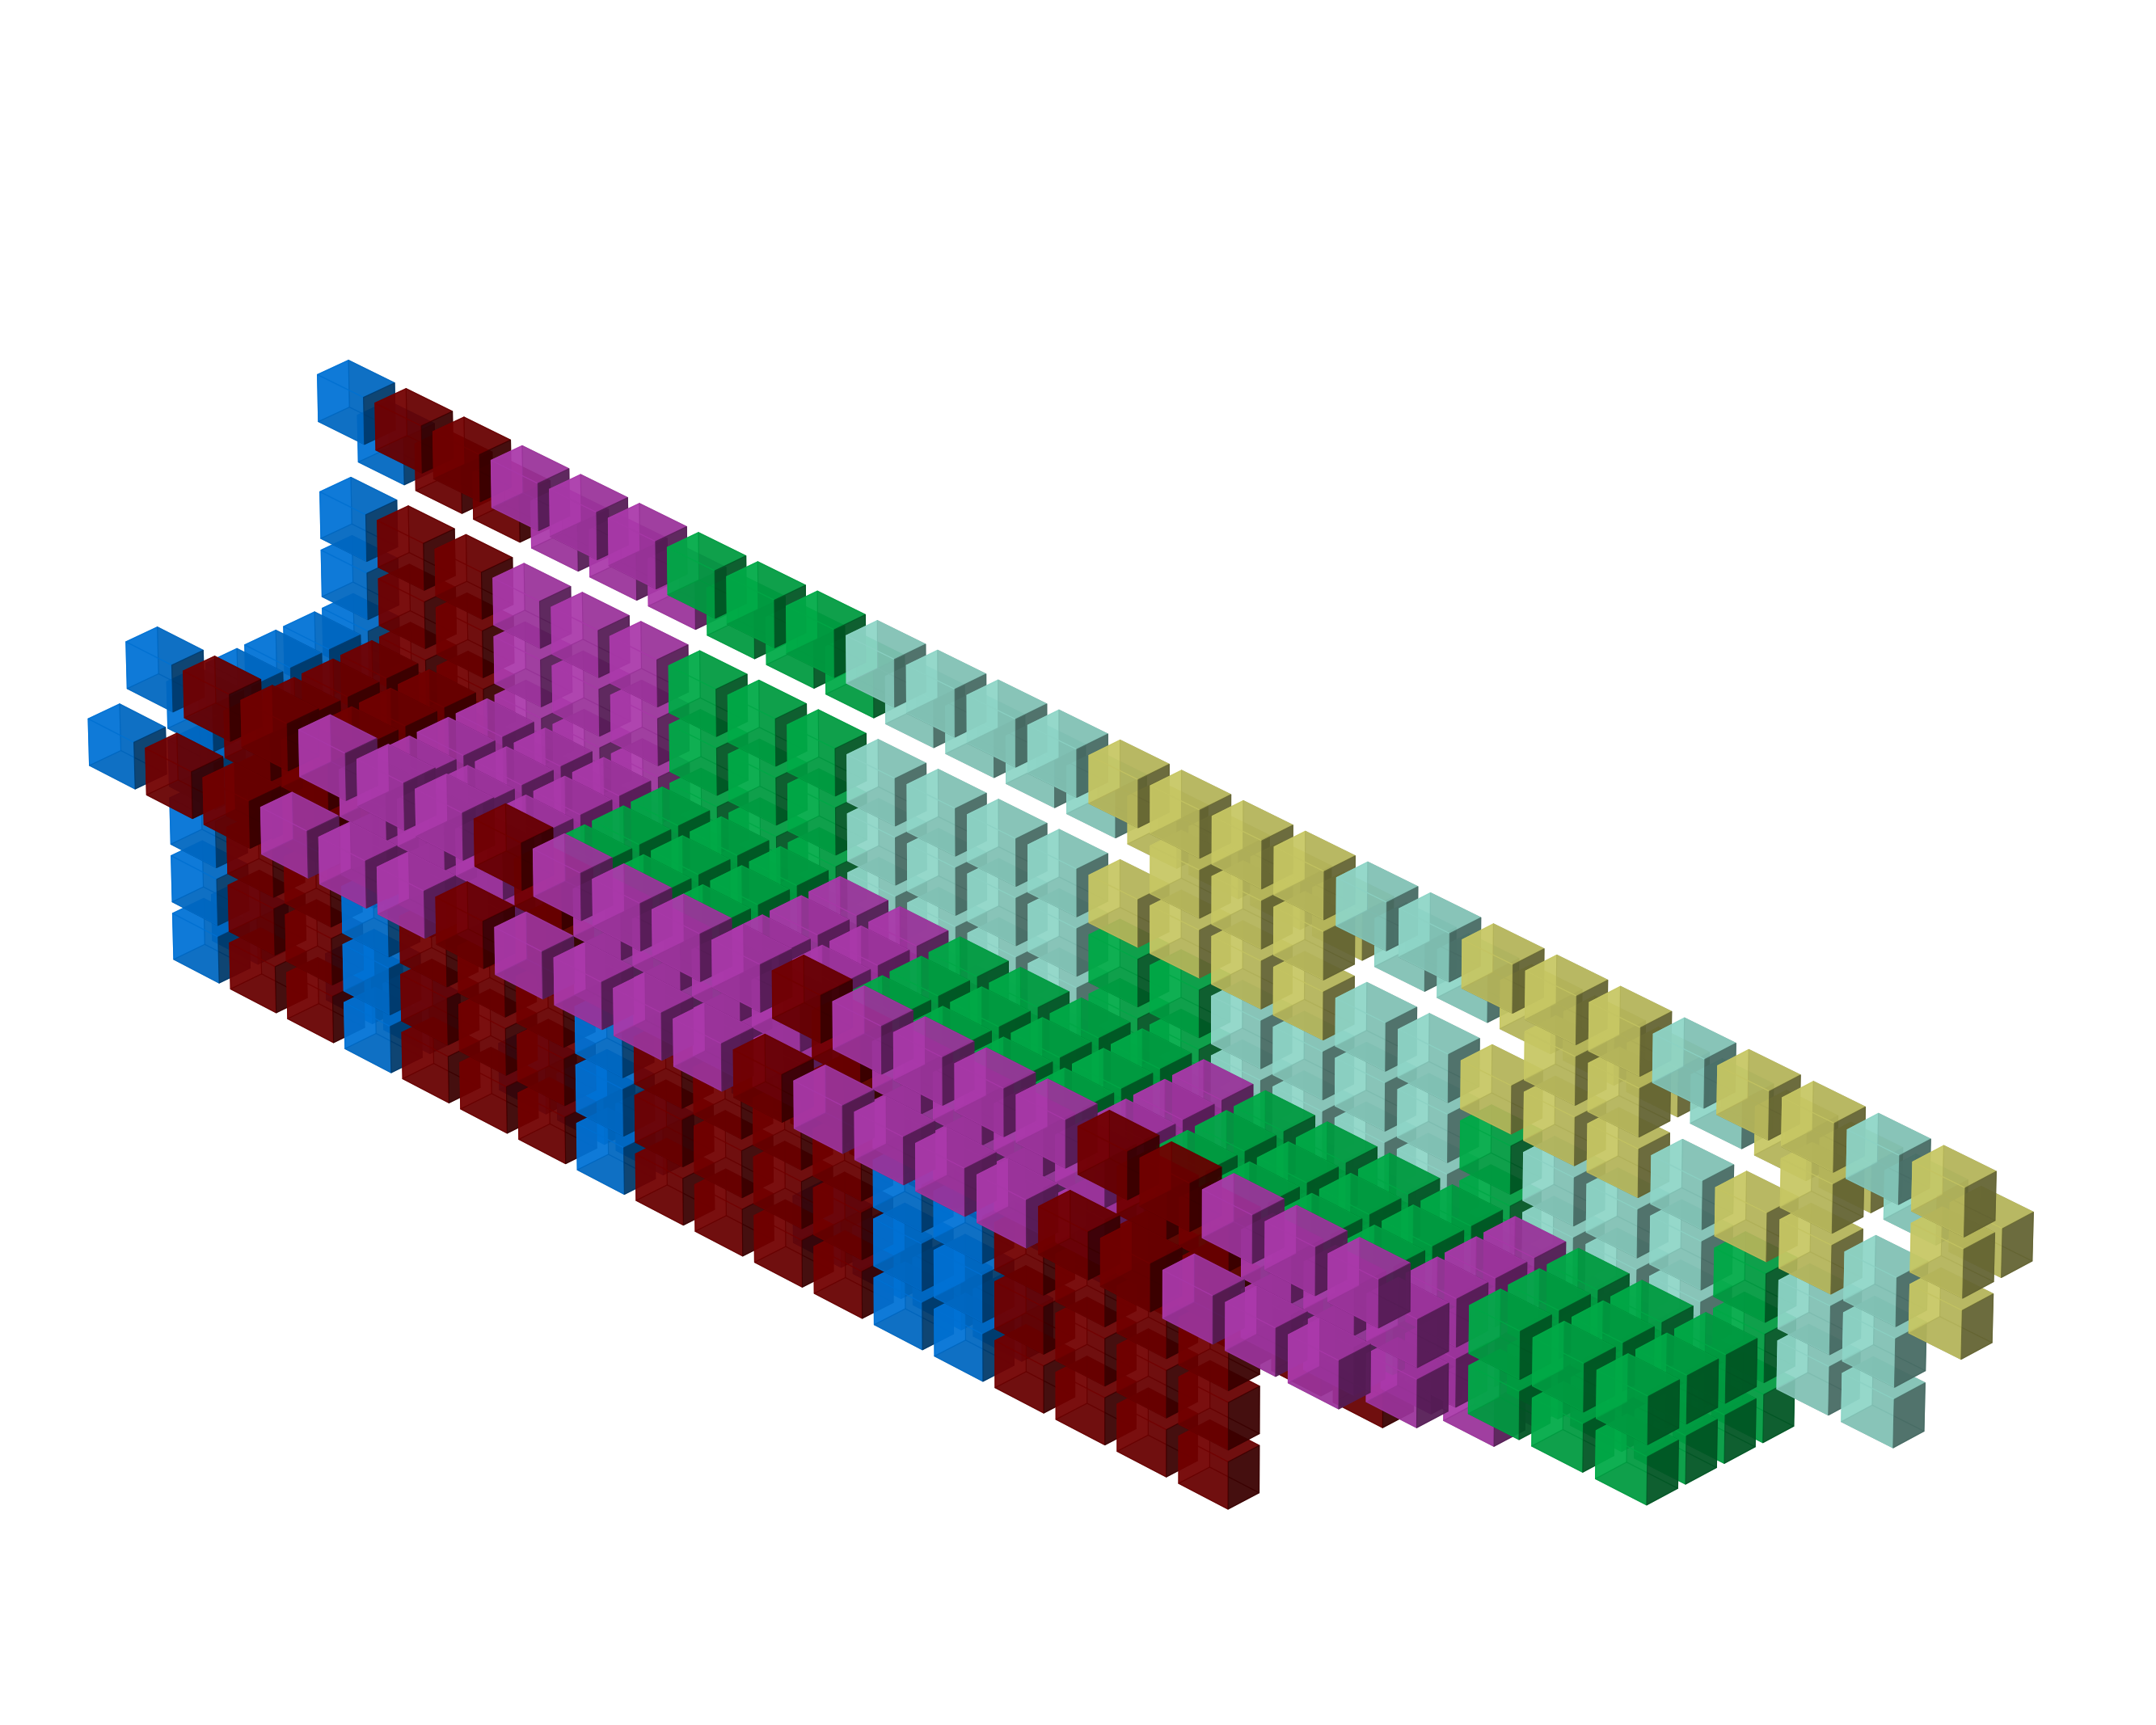
\includegraphics[width=12cm]{src/patterns/pattern2-225.png}%
    \end{adjustbox}
\caption{'La Llamita'.}
\end{figure}
\clearpage

\begin{lstlisting}
laLlamitaXPosArray  .BYTE $00,$FF,$00,$55                    ;  0       
                    .BYTE $00,$00,$55                        ; 06      
                    .BYTE $01,$02,$03,$00,$01,$02,$03,$55    ;  0      
                    .BYTE $04,$05,$06,$04,$00,$01,$02,$55    ;  1    3 
                    .BYTE $04,$00,$04,$00,$04,$55            ;  12223 3
                    .BYTE $FF,$03,$55                        ;  22223  
                    .BYTE $00,$55                            ;  333 4  
laLlamitaYPosArray  .BYTE $FF,$00,$01,$55                    ;  4   4  
                    .BYTE $02,$03,$55                        ; 54  54  
                    .BYTE $03,$03,$03,$04,$04,$04,$04,$55
                    .BYTE $03,$02,$03,$04,$05,$05,$05,$55
                    .BYTE $05,$06,$06,$07,$07,$55
                    .BYTE $07,$07,$55
                    .BYTE $00,$55

\end{lstlisting}
\subfile{patterns/tables/pattern2.tex}

\clearpage
\begin{lstlisting}[basicstyle=\ttfamily\scriptsize]
;-------------------------------------------------------
; CheckKeyboardInput
;-------------------------------------------------------
CheckKeyboardInput   
        ...
CheckForKeyStroke   
        LDA lastKeyPressed
        CMP #$40
        BNE ProcessKeyStroke

        ; No key was pressed. Return early.
        LDA #$00
        STA timerBetweenKeyStrokes
        JSR DisplayDemoModeMessage
ReturnFromKeyboardCheck   
        RTS 

        ; A key was pressed. Figure out which one.
ProcessKeyStroke   
        LDY initialTimeBetweenKeyStrokes
        STY timerBetweenKeyStrokes
        LDY shiftKey
        STY shiftPressed

        CMP #KEY_SPACE ; Space pressed?
        BNE MaybeSPressed

SpacePressed
        ; Space pressed. Selects a new pattern element. "There are
        ; eight permanent ones, and eight you can define for yourself
        ; (more on this later!). The latter eight are all set up when
        ; you load, so you can always choose from 16 shapes."
        INC currentPatternElement
        LDA currentPatternElement
        AND #$0F
        STA currentPatternElement
        AND #$08
        BEQ UpdateCurrentPattern
        ; The first 8 patterns are standard, the rest are custom.
        JMP GetCustomPatternElement
UpdateCurrentPattern   
        JSR ClearLastLineOfScreen
        LDA currentPatternElement
        ASL 
        ASL 
        ASL 
        ASL 
        TAY 

        LDX #$00
txtPresetLoop   
        LDA txtPresetPatternNames,Y
        STA lastLineBufferPtr,X
        INY 
        INX 
        CPX #$10
        BNE txtPresetLoop
        JMP WriteLastLineBufferToScreen
        ; Returns
\end{lstlisting}
\clearpage

\textbf{Lines 1189-1231. \icode{\textbf{SpacePressed}}:} This is the routine that detects when the player has selected a new
symmetry by pressing the 'S' key. It is part of the much larger routine \icode{CheckKeyboardInput} which periodically checks
for keyboard input by polling the byte at address \icode{\$00C5} (which we label \icode{lastKeyPressed}). This address always
contains the value of the most recently pressed key on the keyboard.

If Shift was pressed the user is actually looking to trigger a save, in which case execution passes to \icode{PromptToSave}.

Otherwise we increment \icode{currentSymmetrySetting}, which is the variable we use for storing the currently selected symmetry.
Each press of the 'S' key increments the value of \icode{currentSymmetrySetting} until it reaches 5. Once that happens, we 
reset it to zero again (\icode{LDA \#\$00; STA currentSymmetrySetting}).

\textbf{Lines 1214-1219. \icode{\textbf{SetUpYRegisterToGetText}}:} What is the series of \icode{ASL} instructions doing? A tricky
piece of business of course. We have loaded \icode{currentSymmetrySetting} to the \icode{A} register (\icode{LDA currentSymmetrySetting}) and it has a value between 0 and 4.
\icode{ASL} performs a leftward bit-shift on the \icode{A} register. A single left-shift has an interesting property - it doubles the
value of the byte. A second left-shift will double it again, and so on. So our four {ASL} instructions have the effect of turning 1 into
16, 2 into 32, 3 into 48, and 4 into 64. This has the very useful effect of giving us an index into the description of each symmetry!

\begin{lstlisting}
txtPresetPatternNames
        .TEXT     'STAR ONE        '
        .TEXT     'THE TWIST       '
        .TEXT     'LA LLAMITA      '
        .TEXT     'STAR TWO        '
        .TEXT     'DELTOIDS        '
        .TEXT     'DIFFUSED        '
        .TEXT     'MULTICROSS      '
        .TEXT     'PULSAR          '
\end{lstlisting}

So when we take our resulting value and load it into the \icode{Y} register all our \icode{Write\-Symmetry\-Description} needs to do is start at the 
index given by \icode{Y} and write out the next 16 bytes to the screen, displaying the selected symmetry briefly to the player.
\begin{lstlisting}
        LDA currentPatternElement
        STA patternIndexArray,X
\end{lstlisting}
\clearpage
\begin{figure}[H]
    \centering
    \begin{adjustbox}{width=12cm,center}
      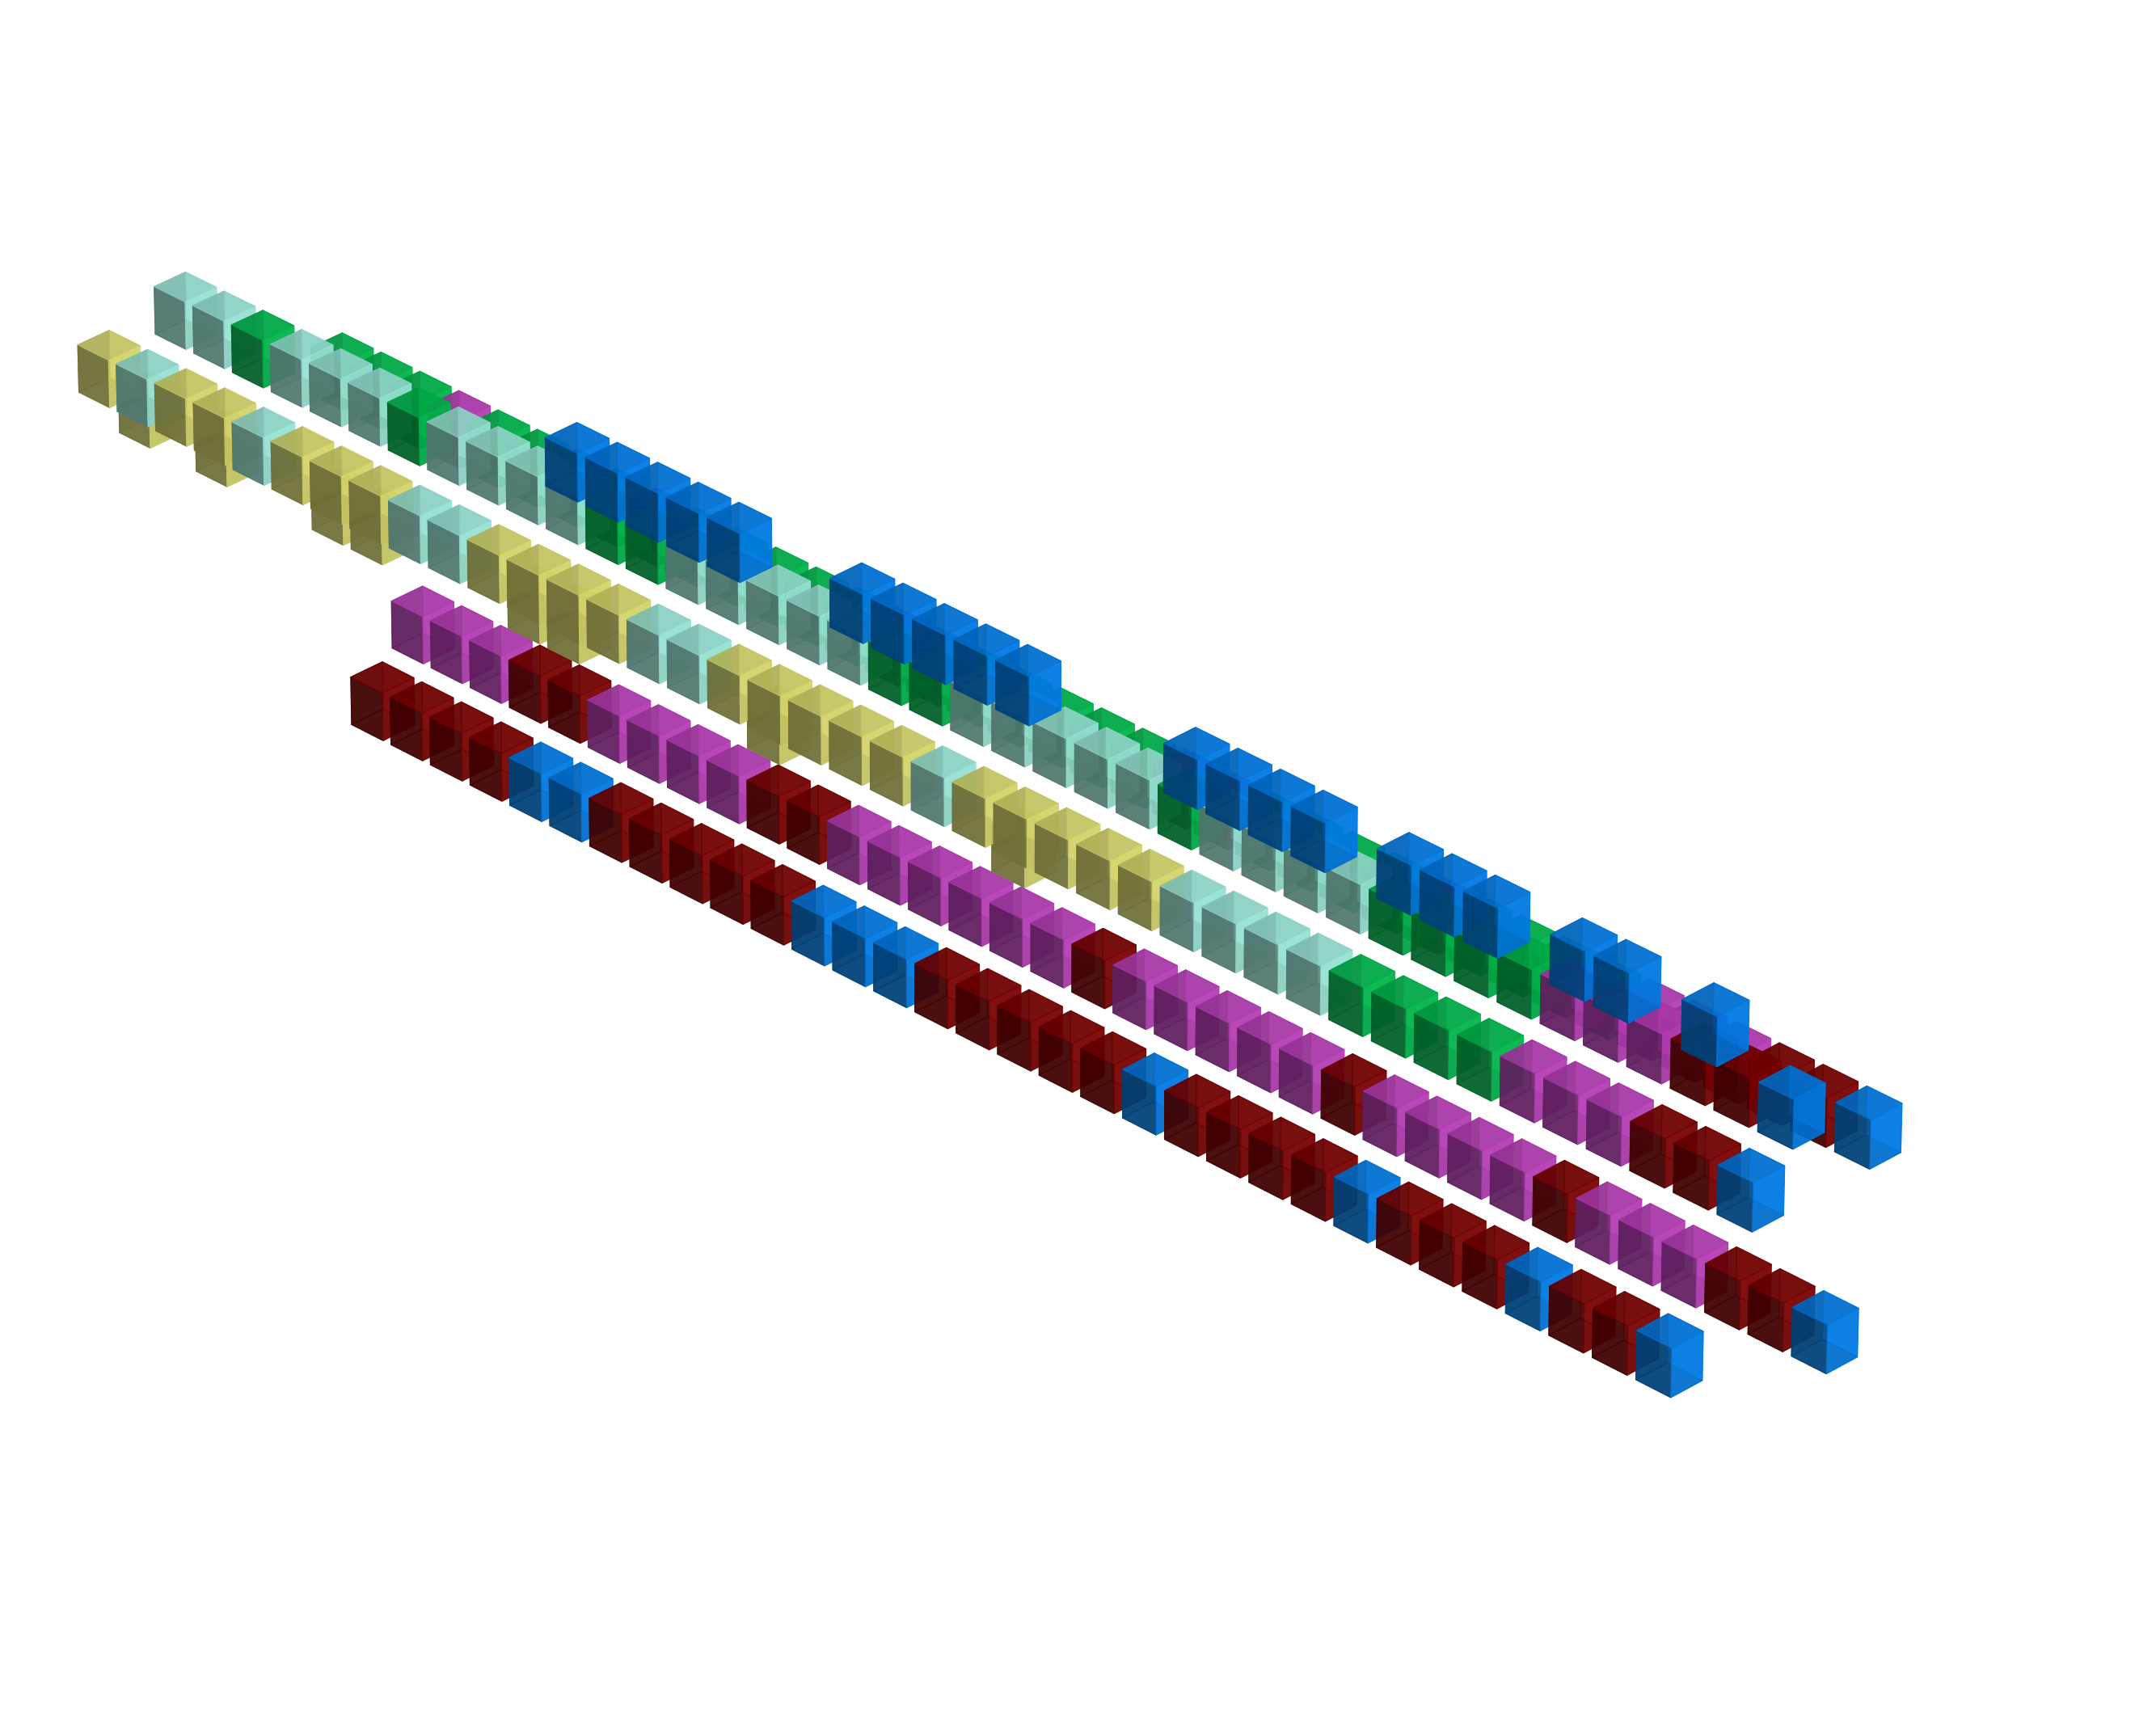
\includegraphics[width=12cm]{src/patterns/pattern3-45.png}%
    \end{adjustbox}
    \begin{adjustbox}{width=12cm,margin=0cm -4cm}
      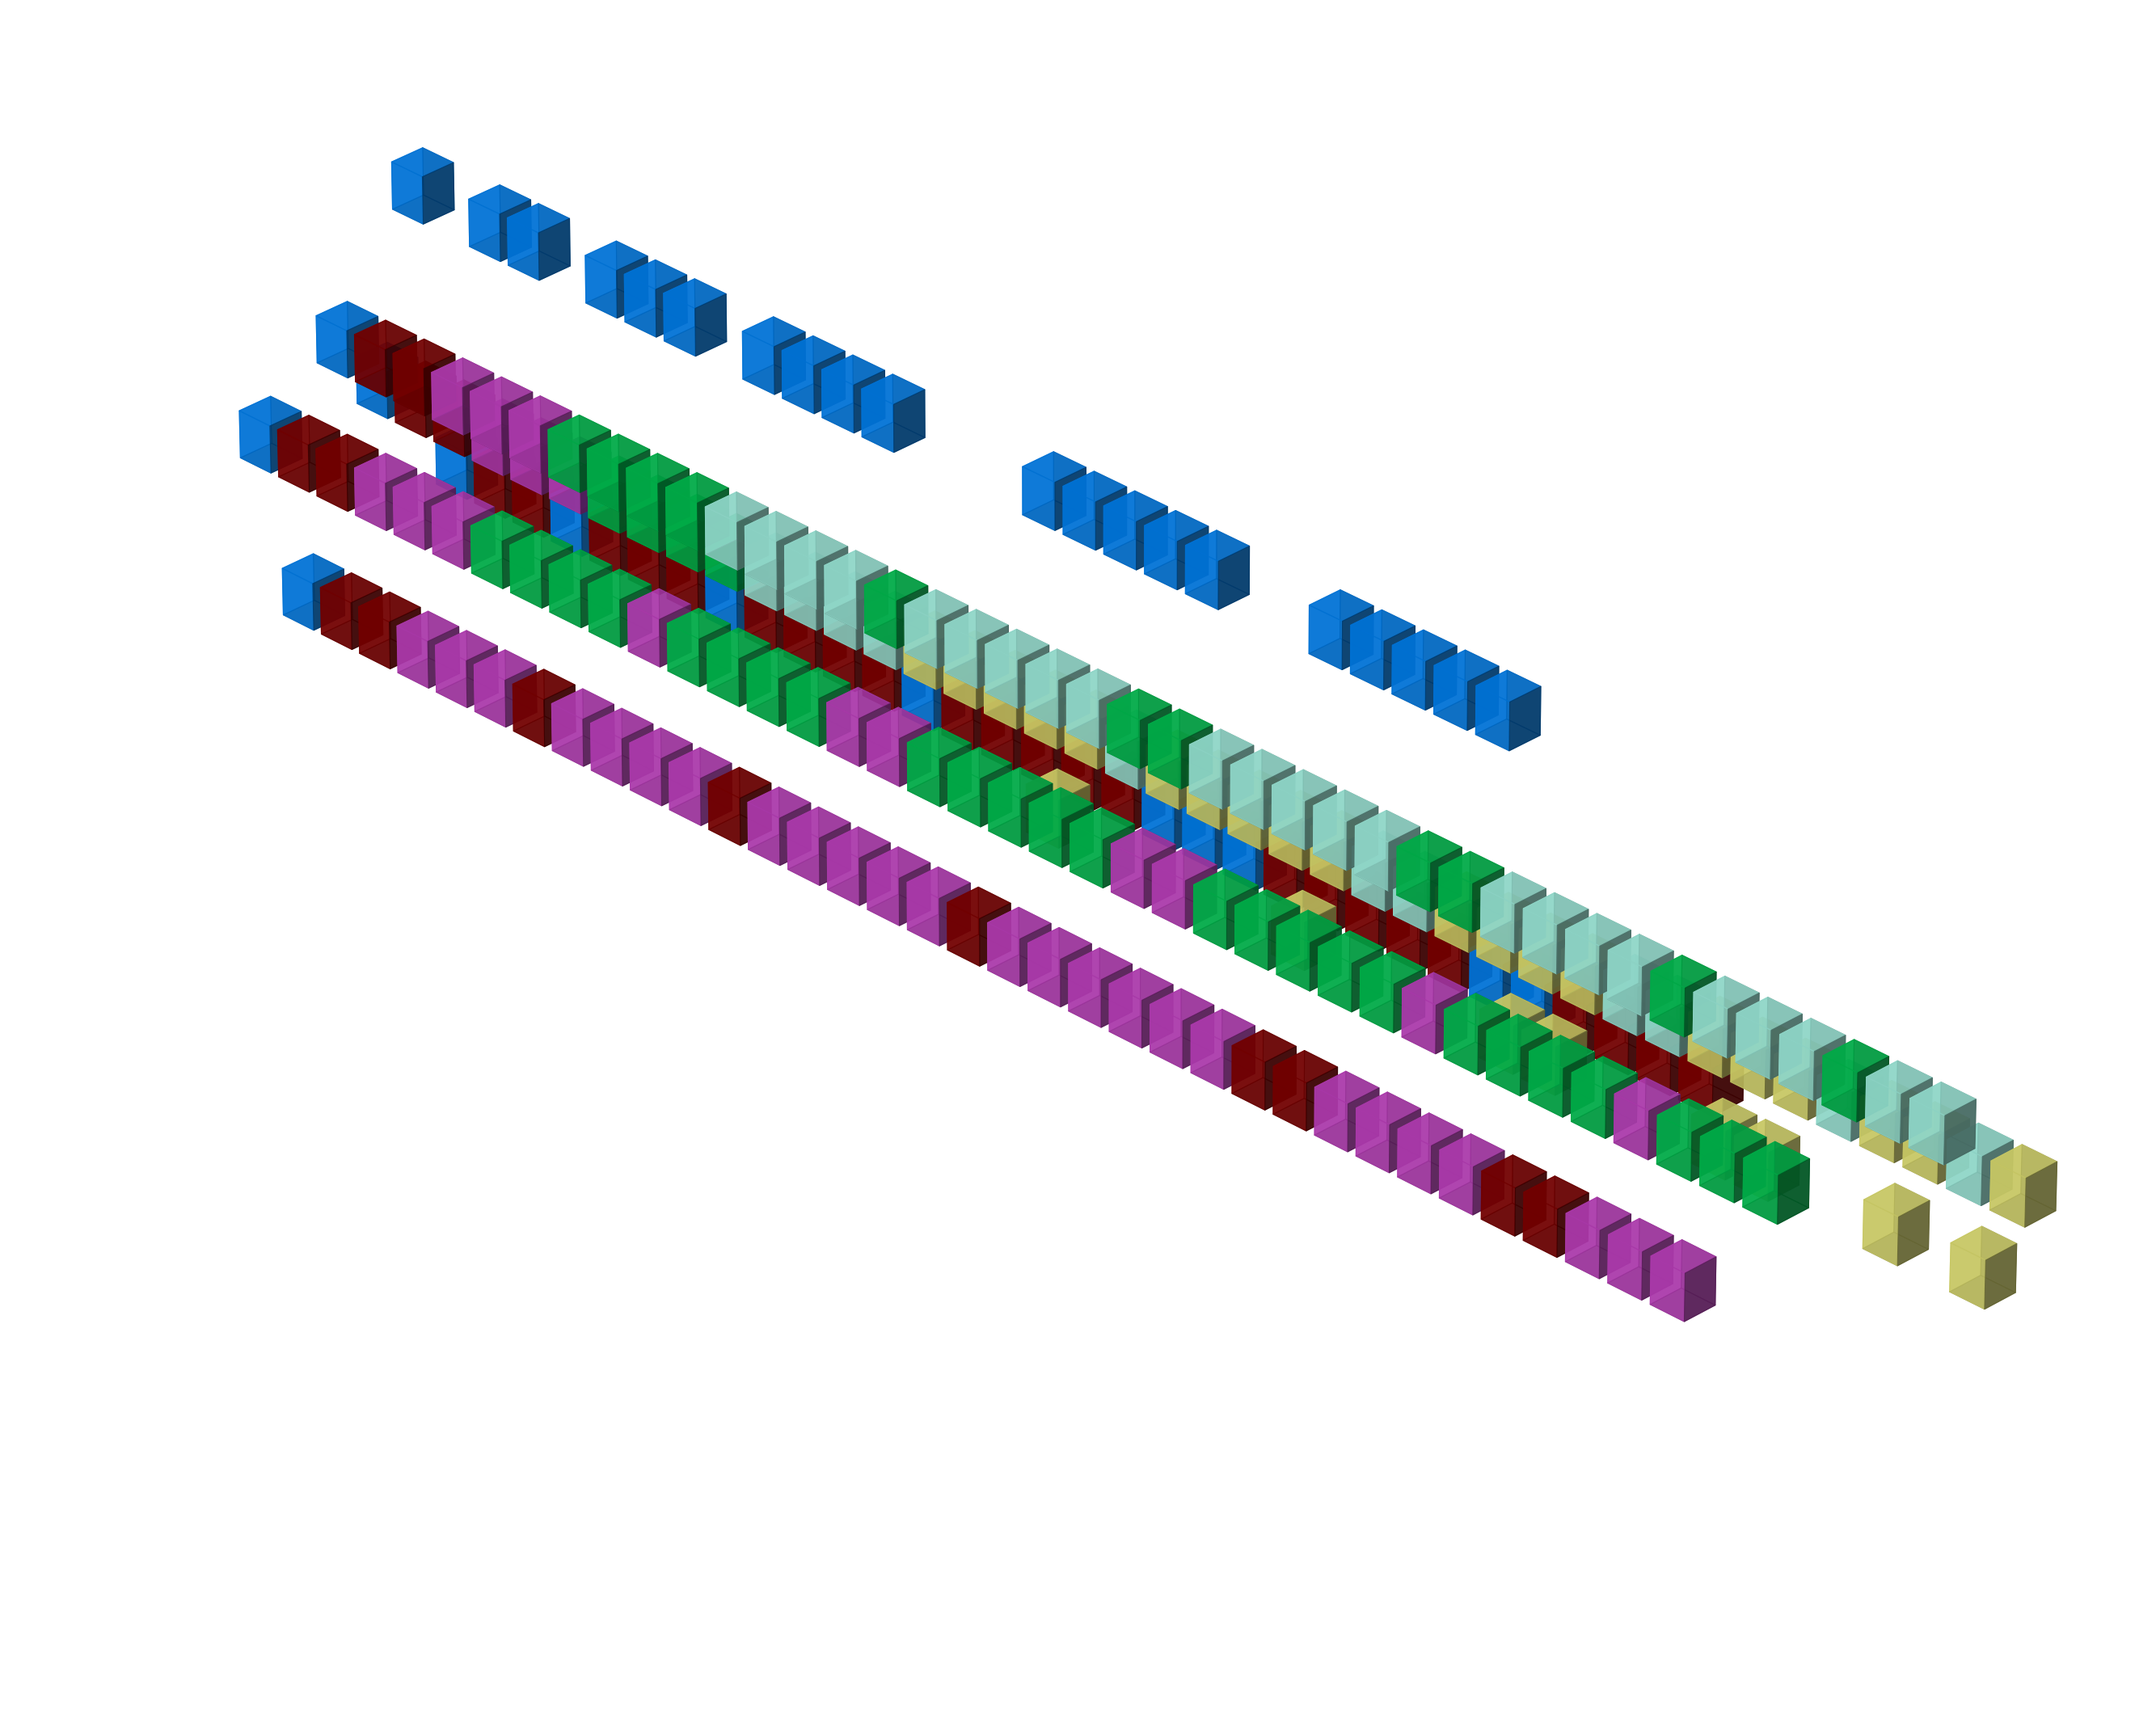
\includegraphics[width=12cm]{src/patterns/pattern3-225.png}%
    \end{adjustbox}
\caption{'Star Two'.}
\end{figure}
\clearpage

\begin{lstlisting}
starTwoXPosArray  .BYTE $FF,$55                  ;    1  
                  .BYTE $00,$55                  ;   0  2
                  .BYTE $02,$55                  ;    6  
                  .BYTE $01,$55                  ; 4     
                  .BYTE $FD,$55                  ;     3 
                  .BYTE $FE,$55                  ;  5    
                  .BYTE $00,$55
starTwoYPosArray  .BYTE $FF,$55
                  .BYTE $FE,$55
                  .BYTE $FF,$55
                  .BYTE $02,$55
                  .BYTE $01,$55
                  .BYTE $FC,$55
                  .BYTE $00,$55
\end{lstlisting}
\subfile{patterns/tables/pattern3.tex}
\clearpage
\clearpage

\begin{figure}[H]
    \centering
    \begin{adjustbox}{width=12cm,center}
      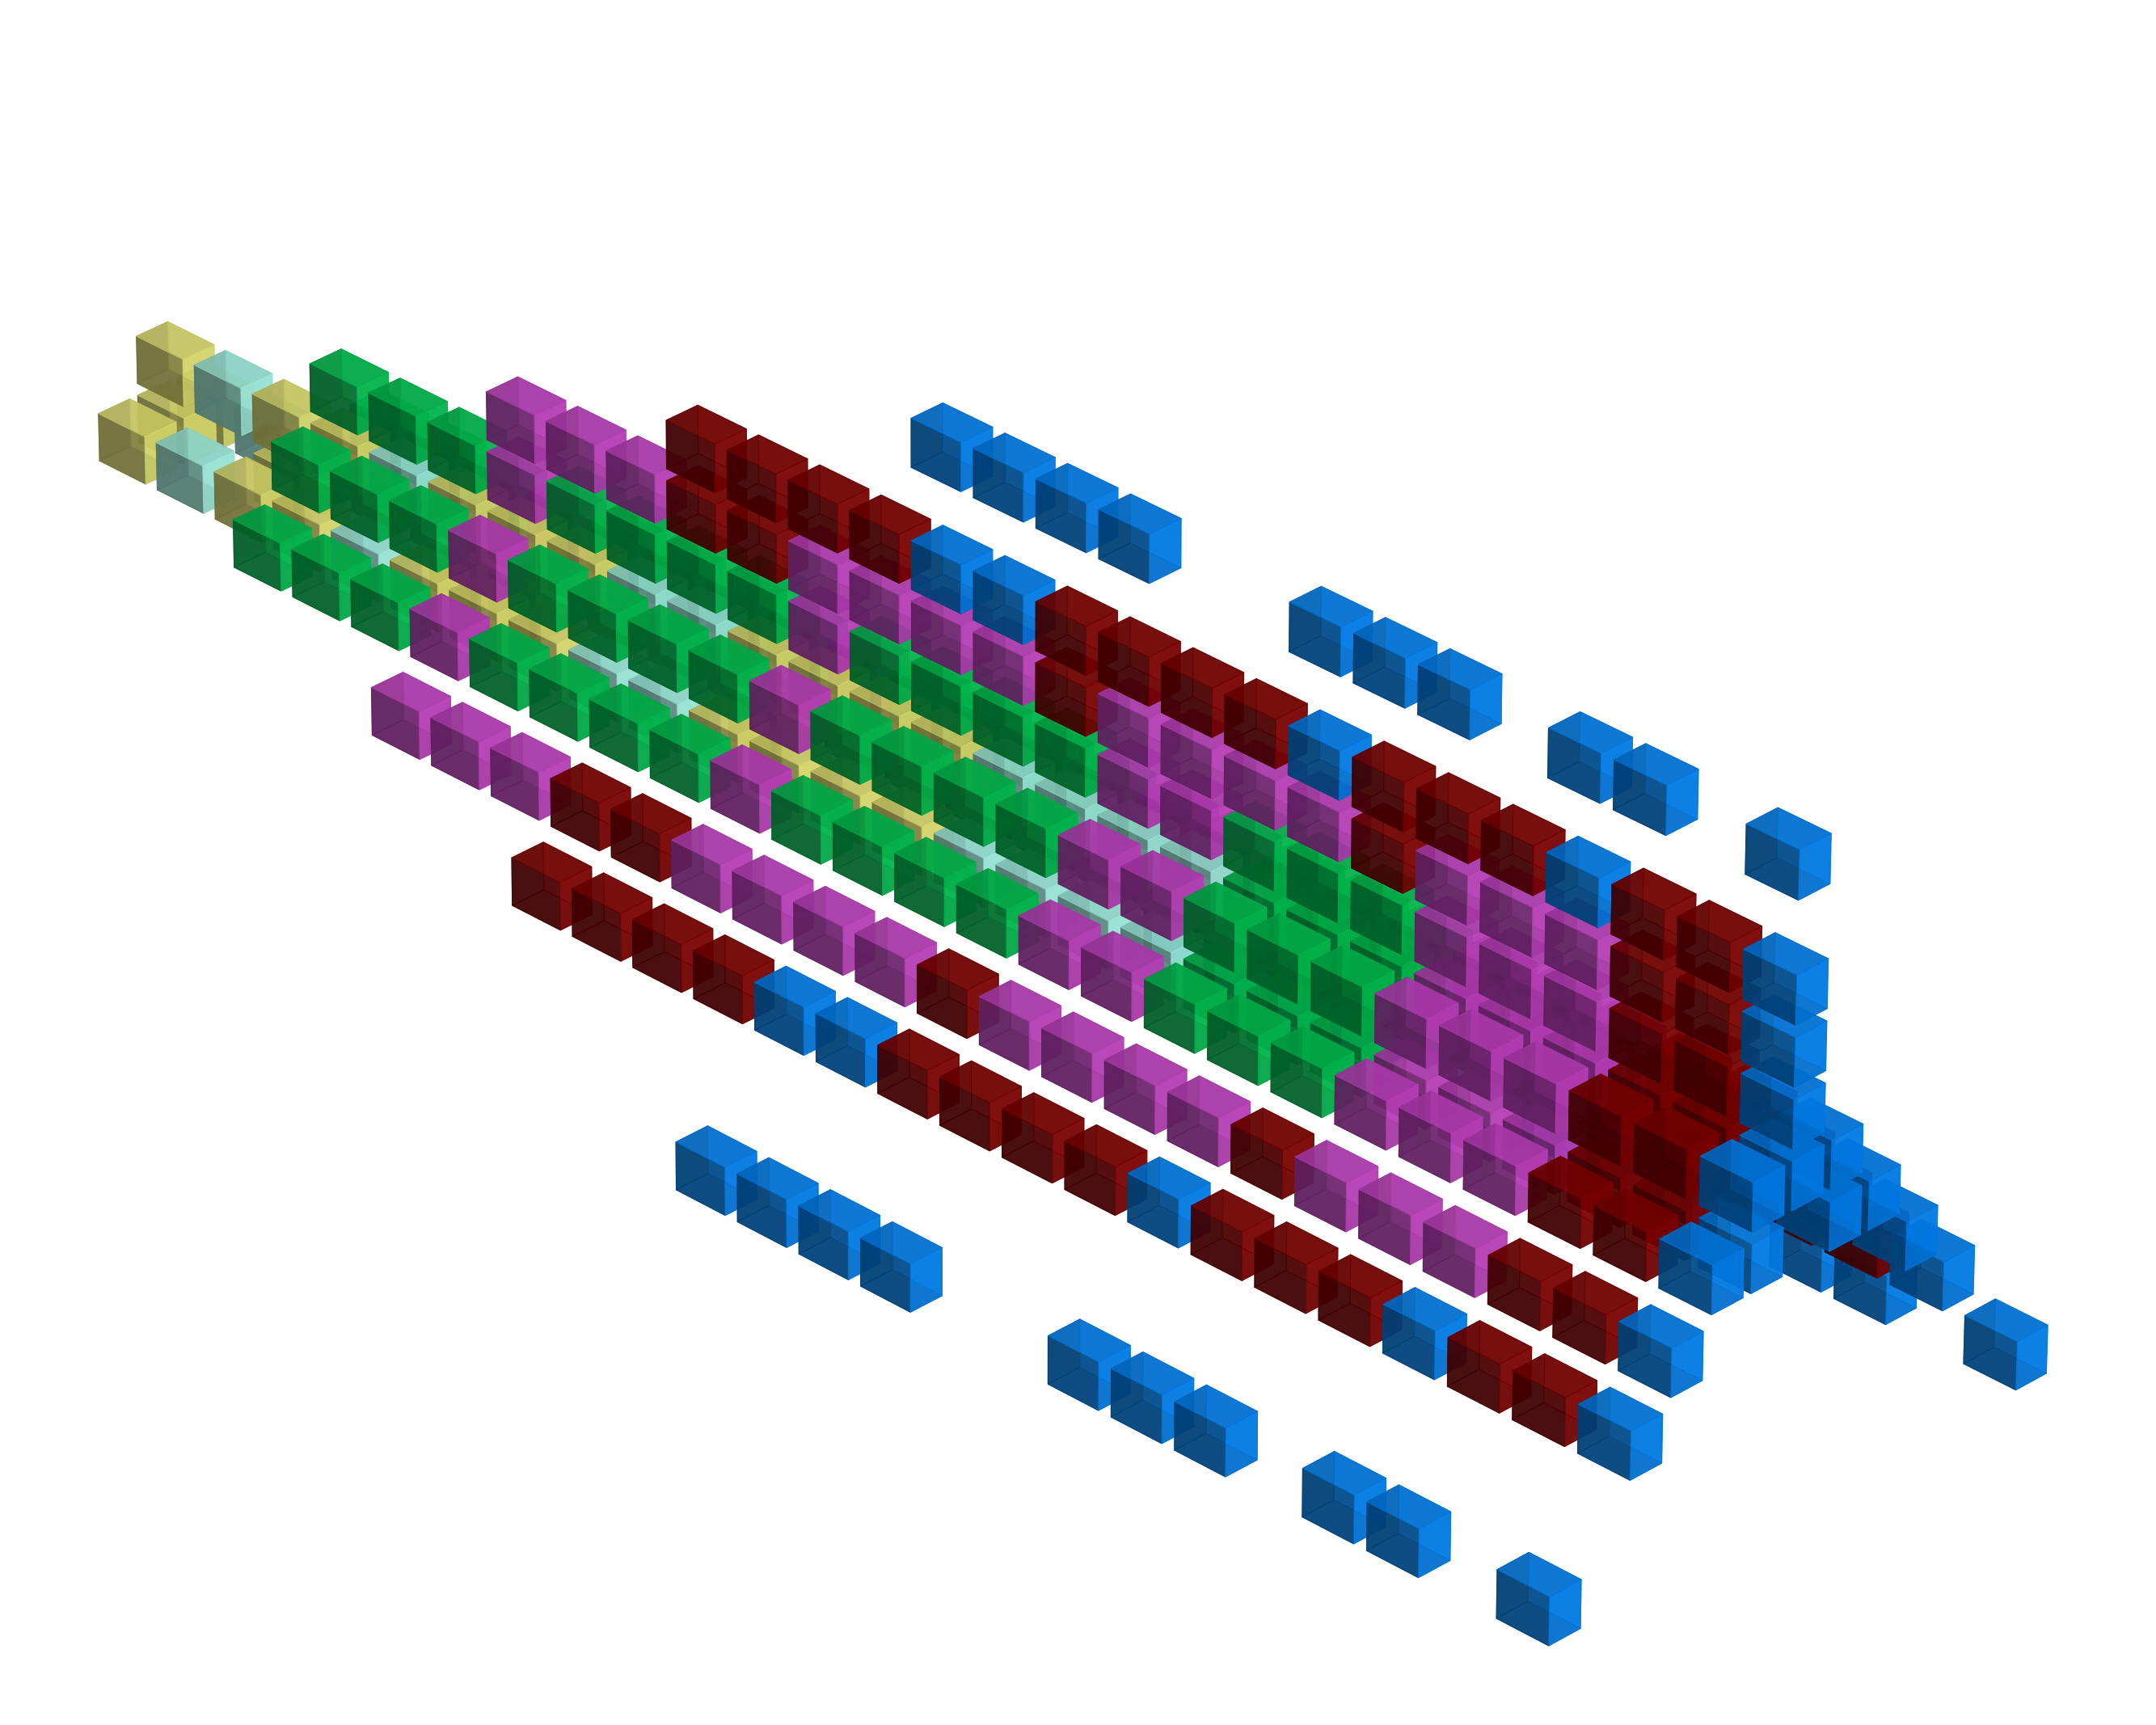
\includegraphics[width=12cm]{src/patterns/pattern4-45.png}%
    \end{adjustbox}
    \begin{adjustbox}{width=12cm,margin=0cm -4cm}
      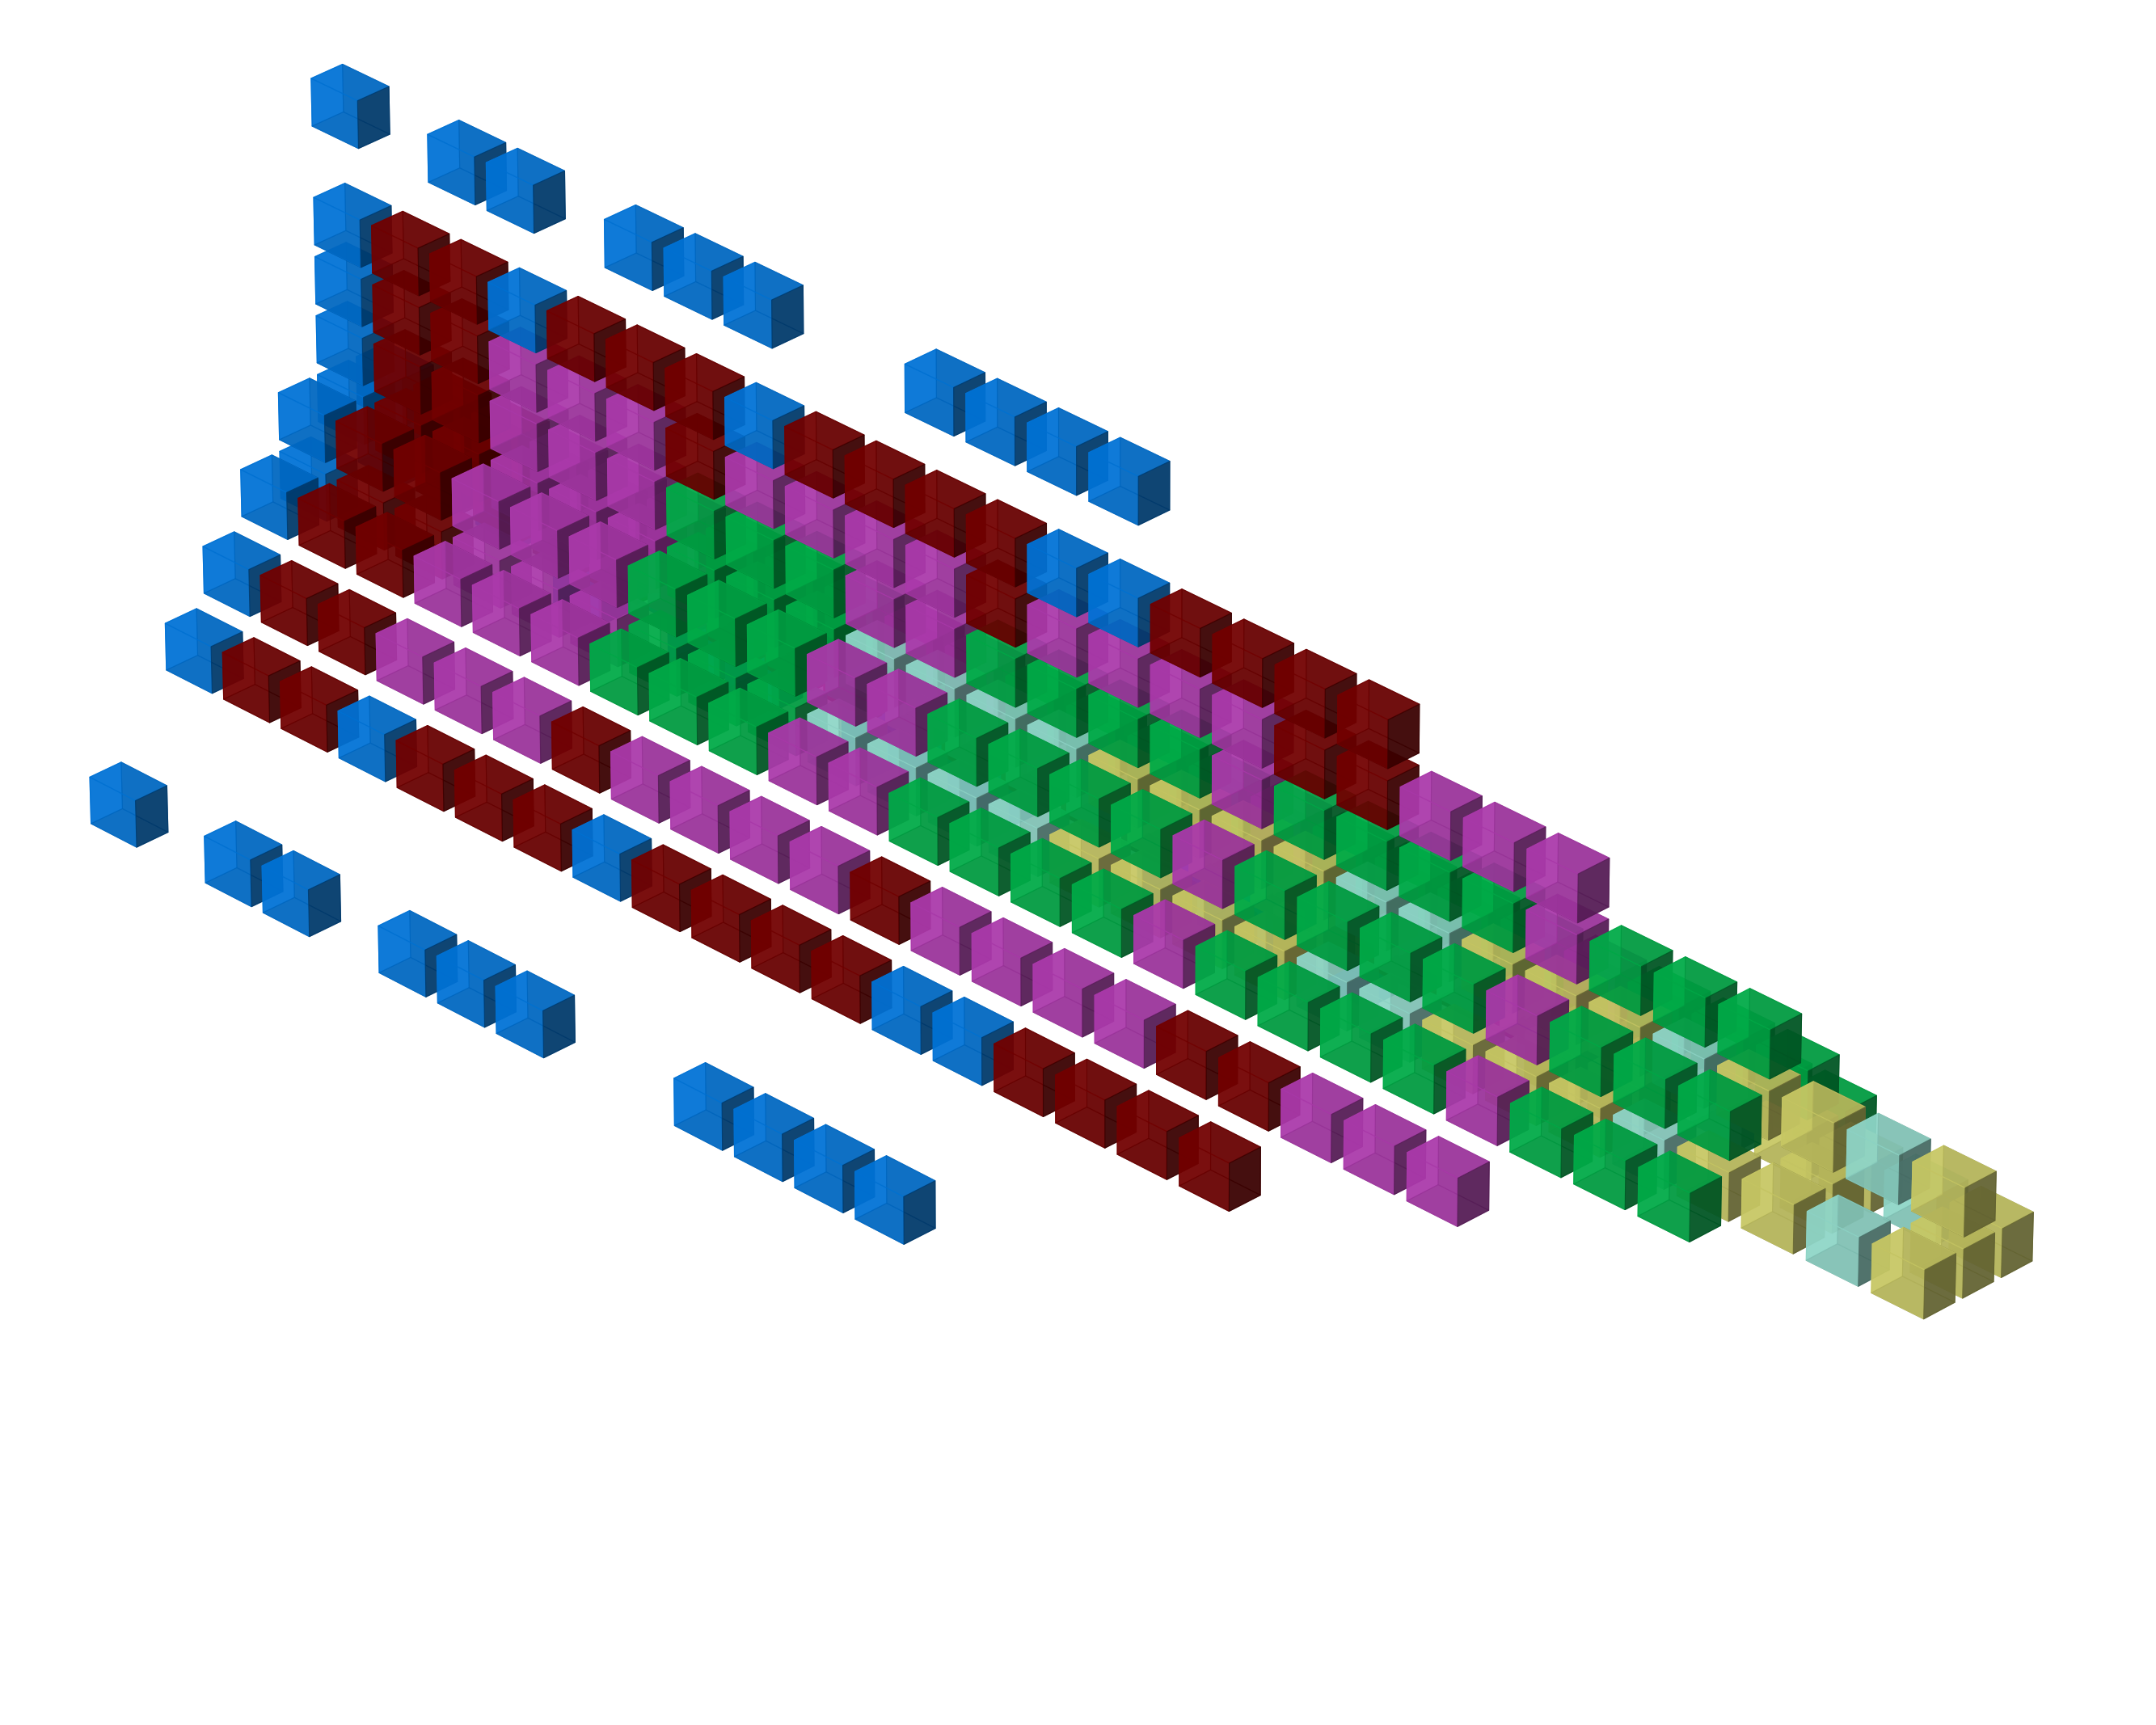
\includegraphics[width=12cm]{src/patterns/pattern4-225.png}%
    \end{adjustbox}
\caption{'Deltoid'.}
\end{figure}
\clearpage

\begin{lstlisting}
deltoidXPosArray  .BYTE $00,$01,$FF,$55           ;       5      
                  .BYTE $00,$55                   ;              
                  .BYTE $00,$01,$02,$FE,$FF,$55   ;       4      
                  .BYTE $00,$03,$FD,$55           ;       3      
                  .BYTE $00,$04,$FC,$55           ;       2      
                  .BYTE $00,$06,$FA,$55           ;      202     
                  .BYTE $00,$55                   ;     20602    
deltoidYPosArray  .BYTE $FF,$00,$00,$55           ;    3     3   
                  .BYTE $00,$55                   ;   4       4  
                  .BYTE $FE,$FF,$00,$00,$FF,$55   ;              
                  .BYTE $FD,$01,$01,$55           ; 5           5
                  .BYTE $FC,$02,$02,$55
                  .BYTE $FA,$04,$04,$55
                  .BYTE $00,$55
\end{lstlisting}
\subfile{patterns/tables/pattern4.tex}

\begin{figure}[H]
    \centering
    \begin{adjustbox}{width=12cm,center}
      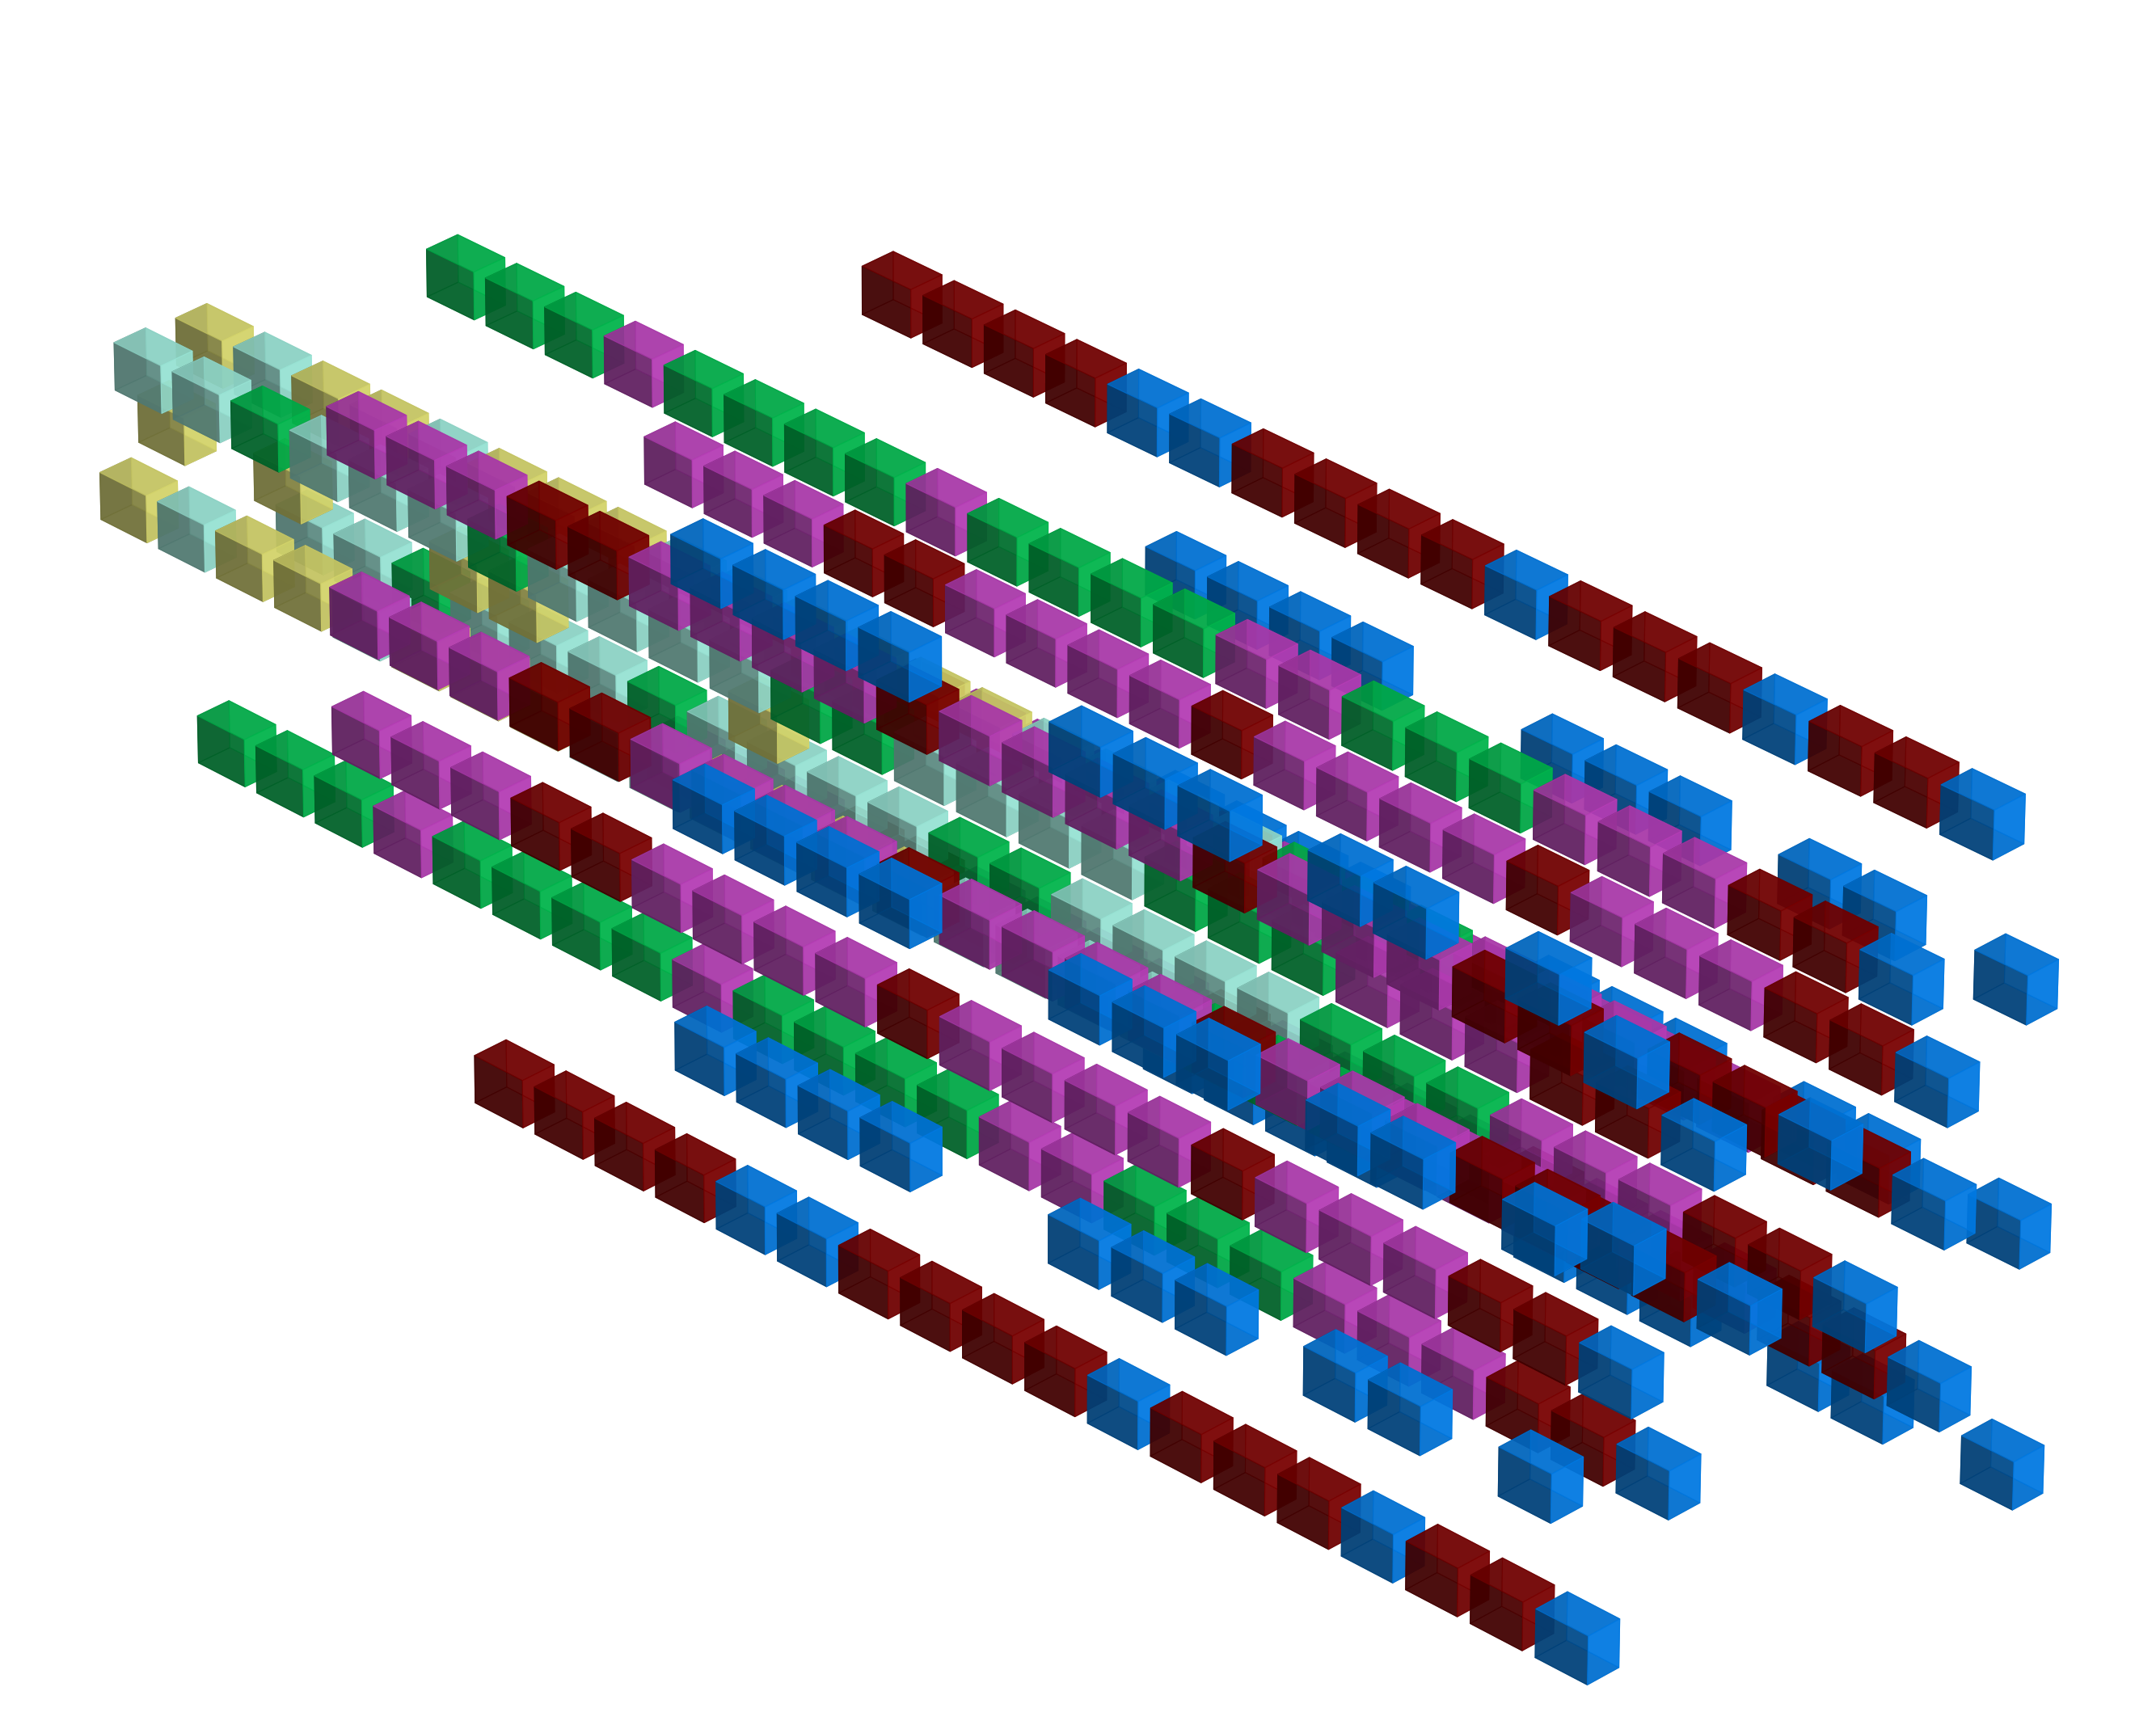
\includegraphics[width=12cm]{src/patterns/pattern5-45.png}%
    \end{adjustbox}
    \begin{adjustbox}{width=12cm,margin=0cm -4cm}
      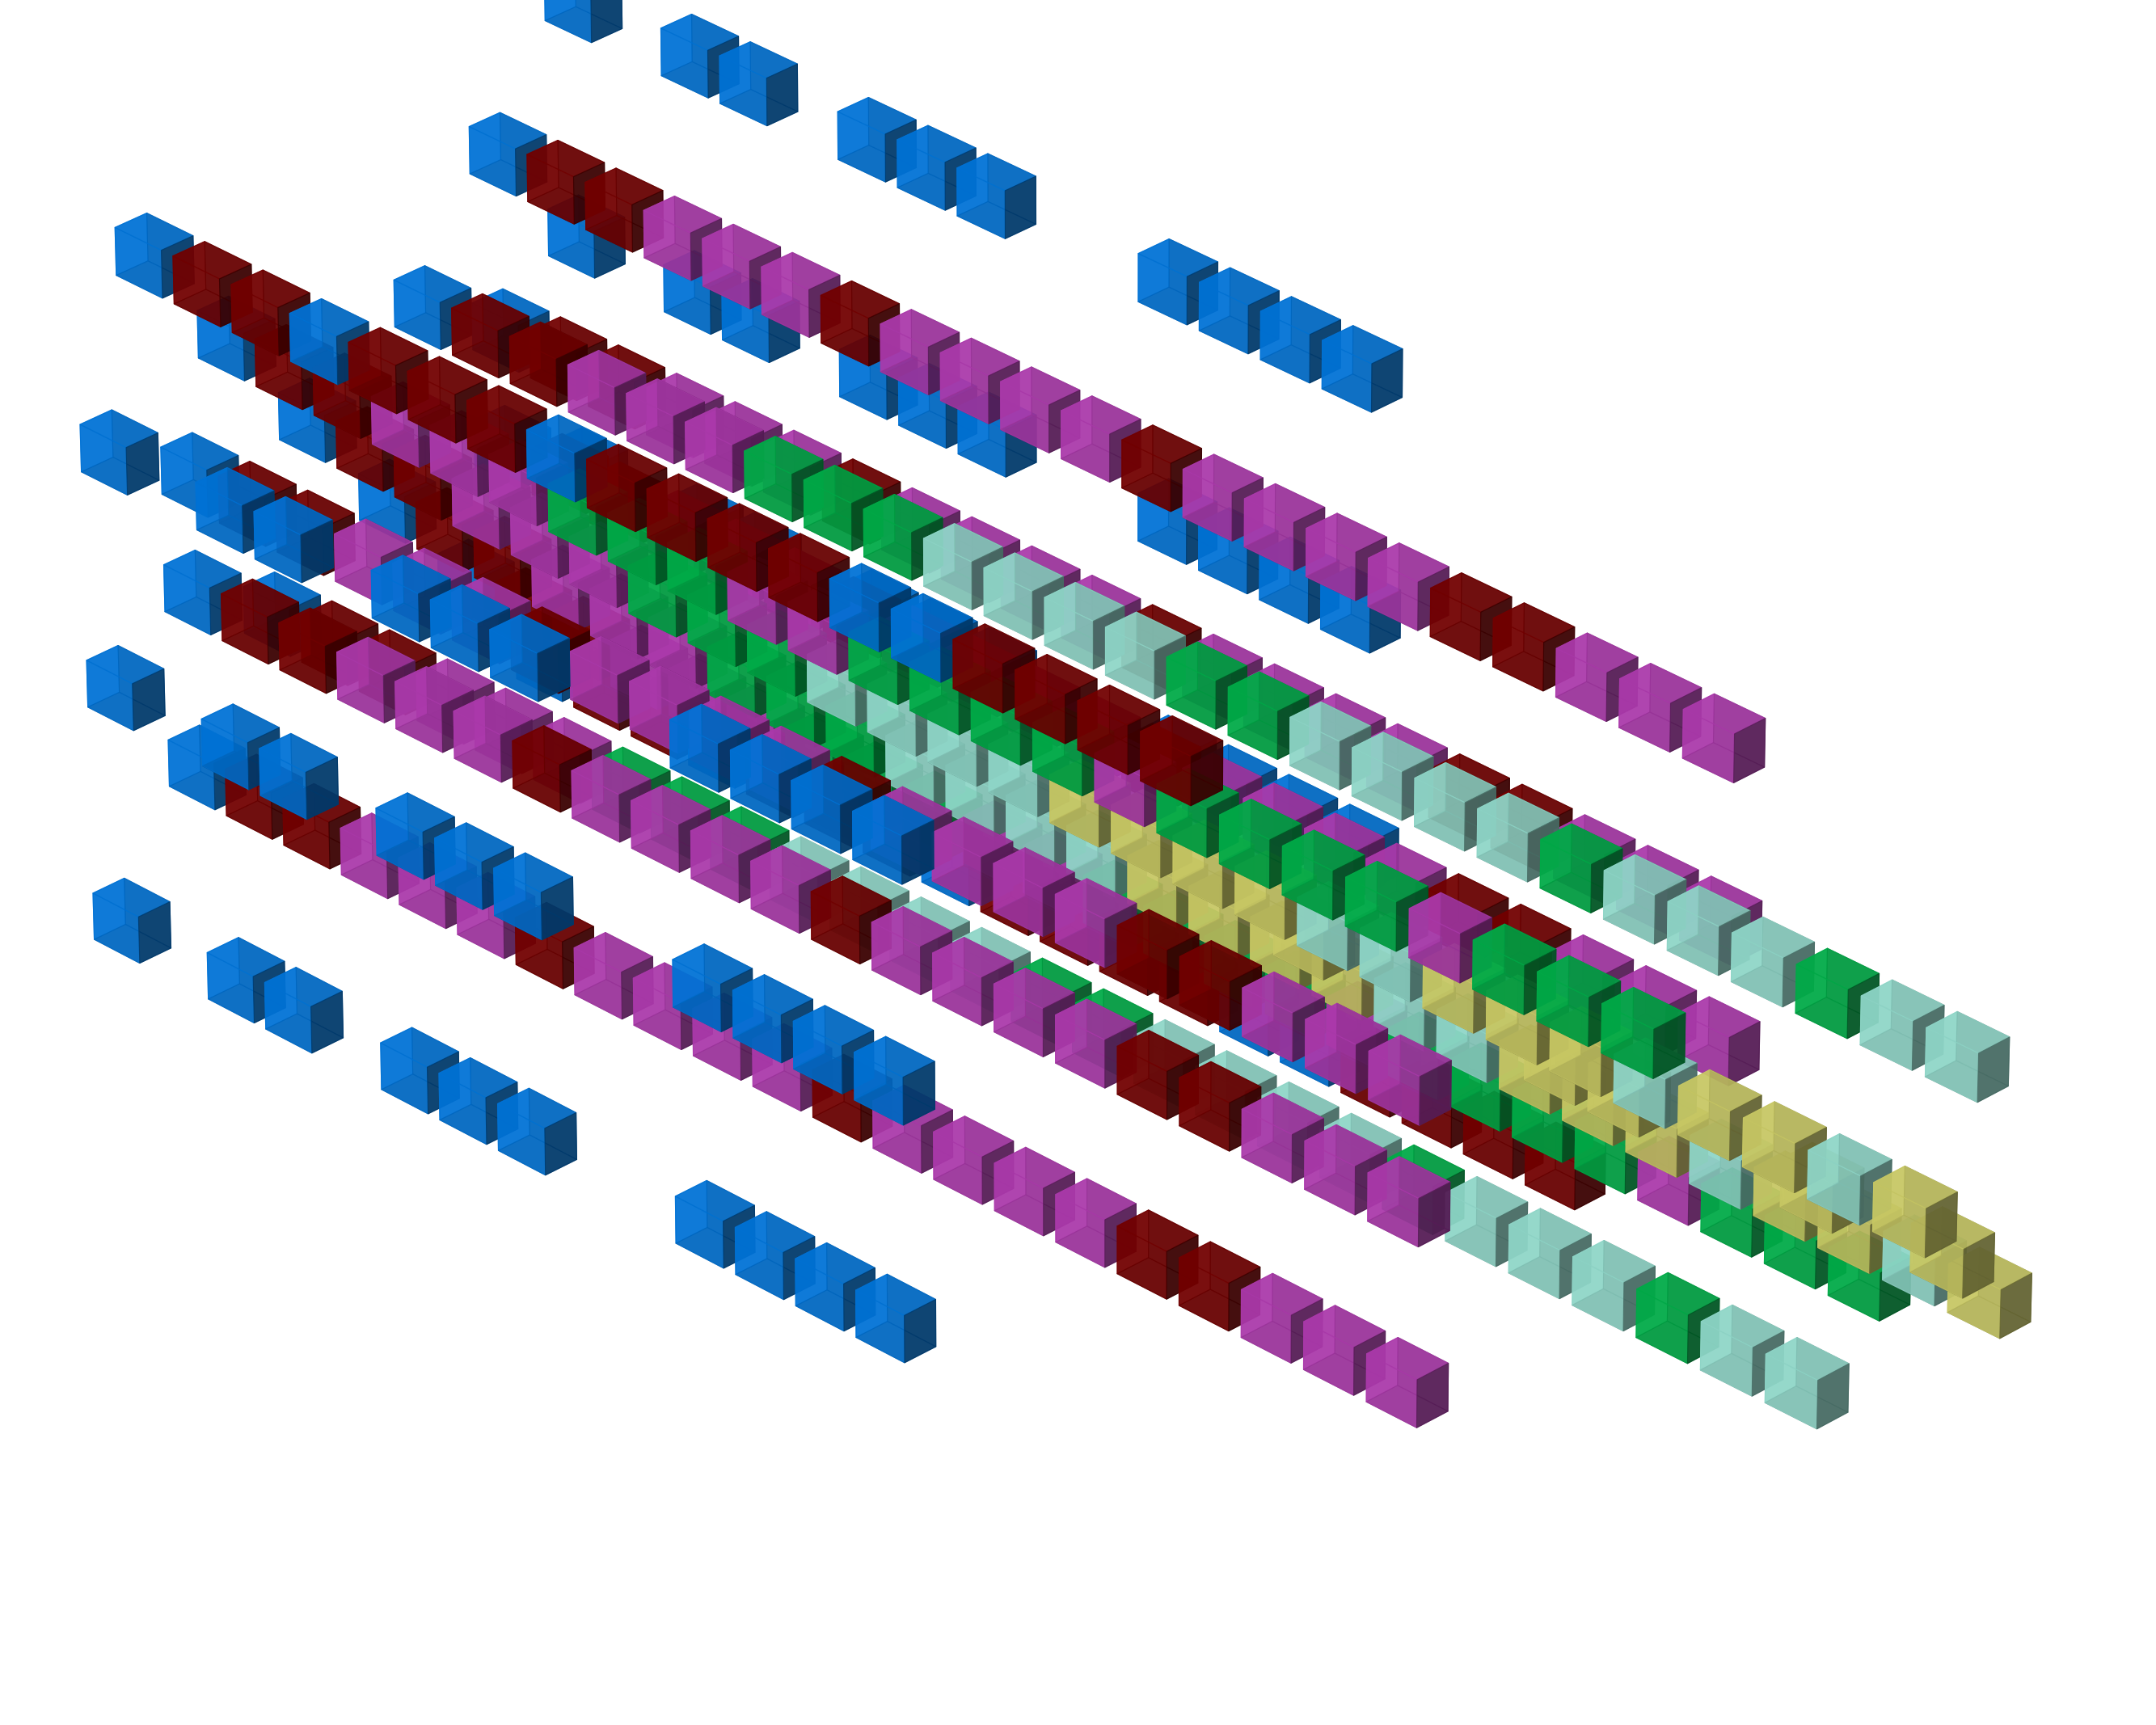
\includegraphics[width=12cm]{src/patterns/pattern5-225.png}%
    \end{adjustbox}
\caption{'Diffused'.}
\end{figure}
\clearpage

\begin{lstlisting}
diffusedXPosArray .BYTE $FF,$01,$55                  ; 5            
                  .BYTE $FE,$02,$55                  ;            4 
                  .BYTE $FD,$03,$55                  ;   3          
                  .BYTE $FC,$04,$FC,$FC,$04,$04,$55  ;          2   
                  .BYTE $FB,$05,$55                  ; 5   1       5
                  .BYTE $FA,$06,$FA,$FA,$06,$06,$55  ;   3    0  3  
                  .BYTE $00,$55                      ;       6      
diffusedYPosArray .BYTE $01,$FF,$55                  ;   3  0    3  
                  .BYTE $FE,$02,$55                  ; 5       1   5
                  .BYTE $03,$FD,$55                  ;    2         
                  .BYTE $FC,$04,$FF,$01,$FF,$01,$55  ;           3  
                  .BYTE $05,$FB,$55                  ;  4           
                  .BYTE $FA,$06,$FE,$02,$FE,$02,$55  ;             5
                  .BYTE $00,$55
\end{lstlisting}
\subfile{patterns/tables/pattern5.tex}

\begin{figure}[H]
    \centering
    \begin{adjustbox}{width=12cm,center}
      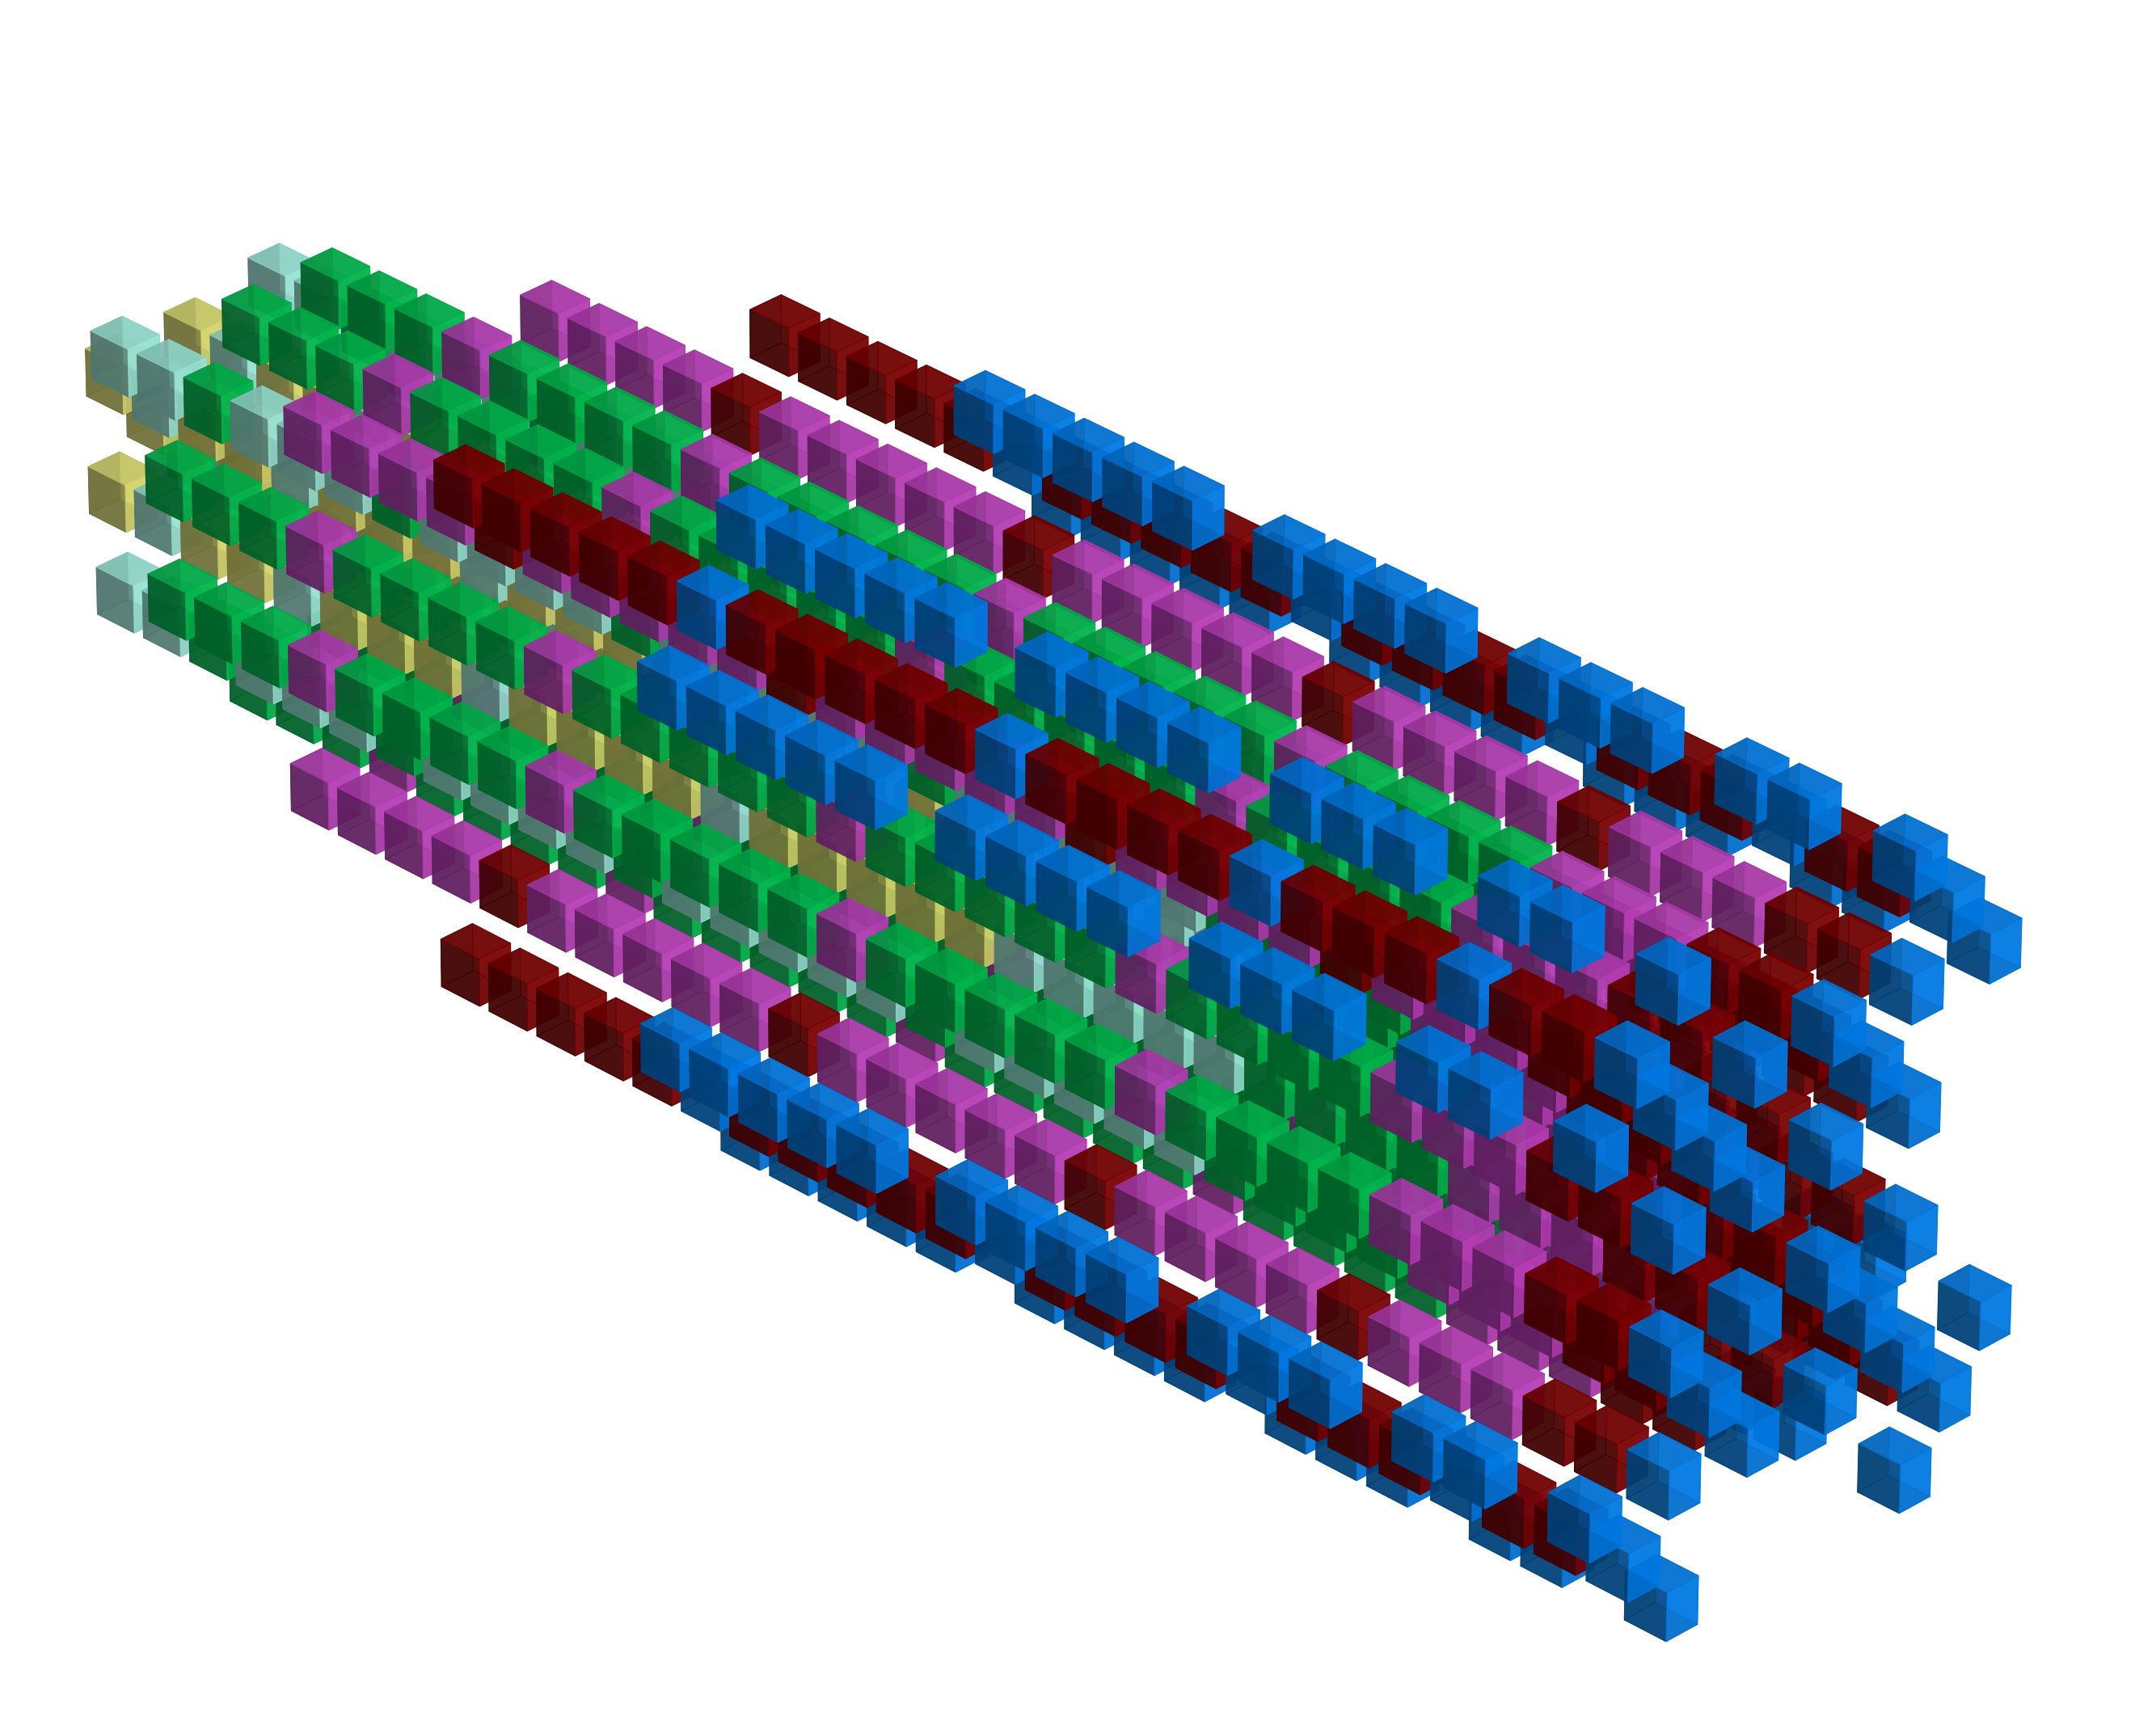
\includegraphics[width=12cm]{src/patterns/pattern6-45.png}%
    \end{adjustbox}
    \begin{adjustbox}{width=12cm,margin=0cm -4cm}
      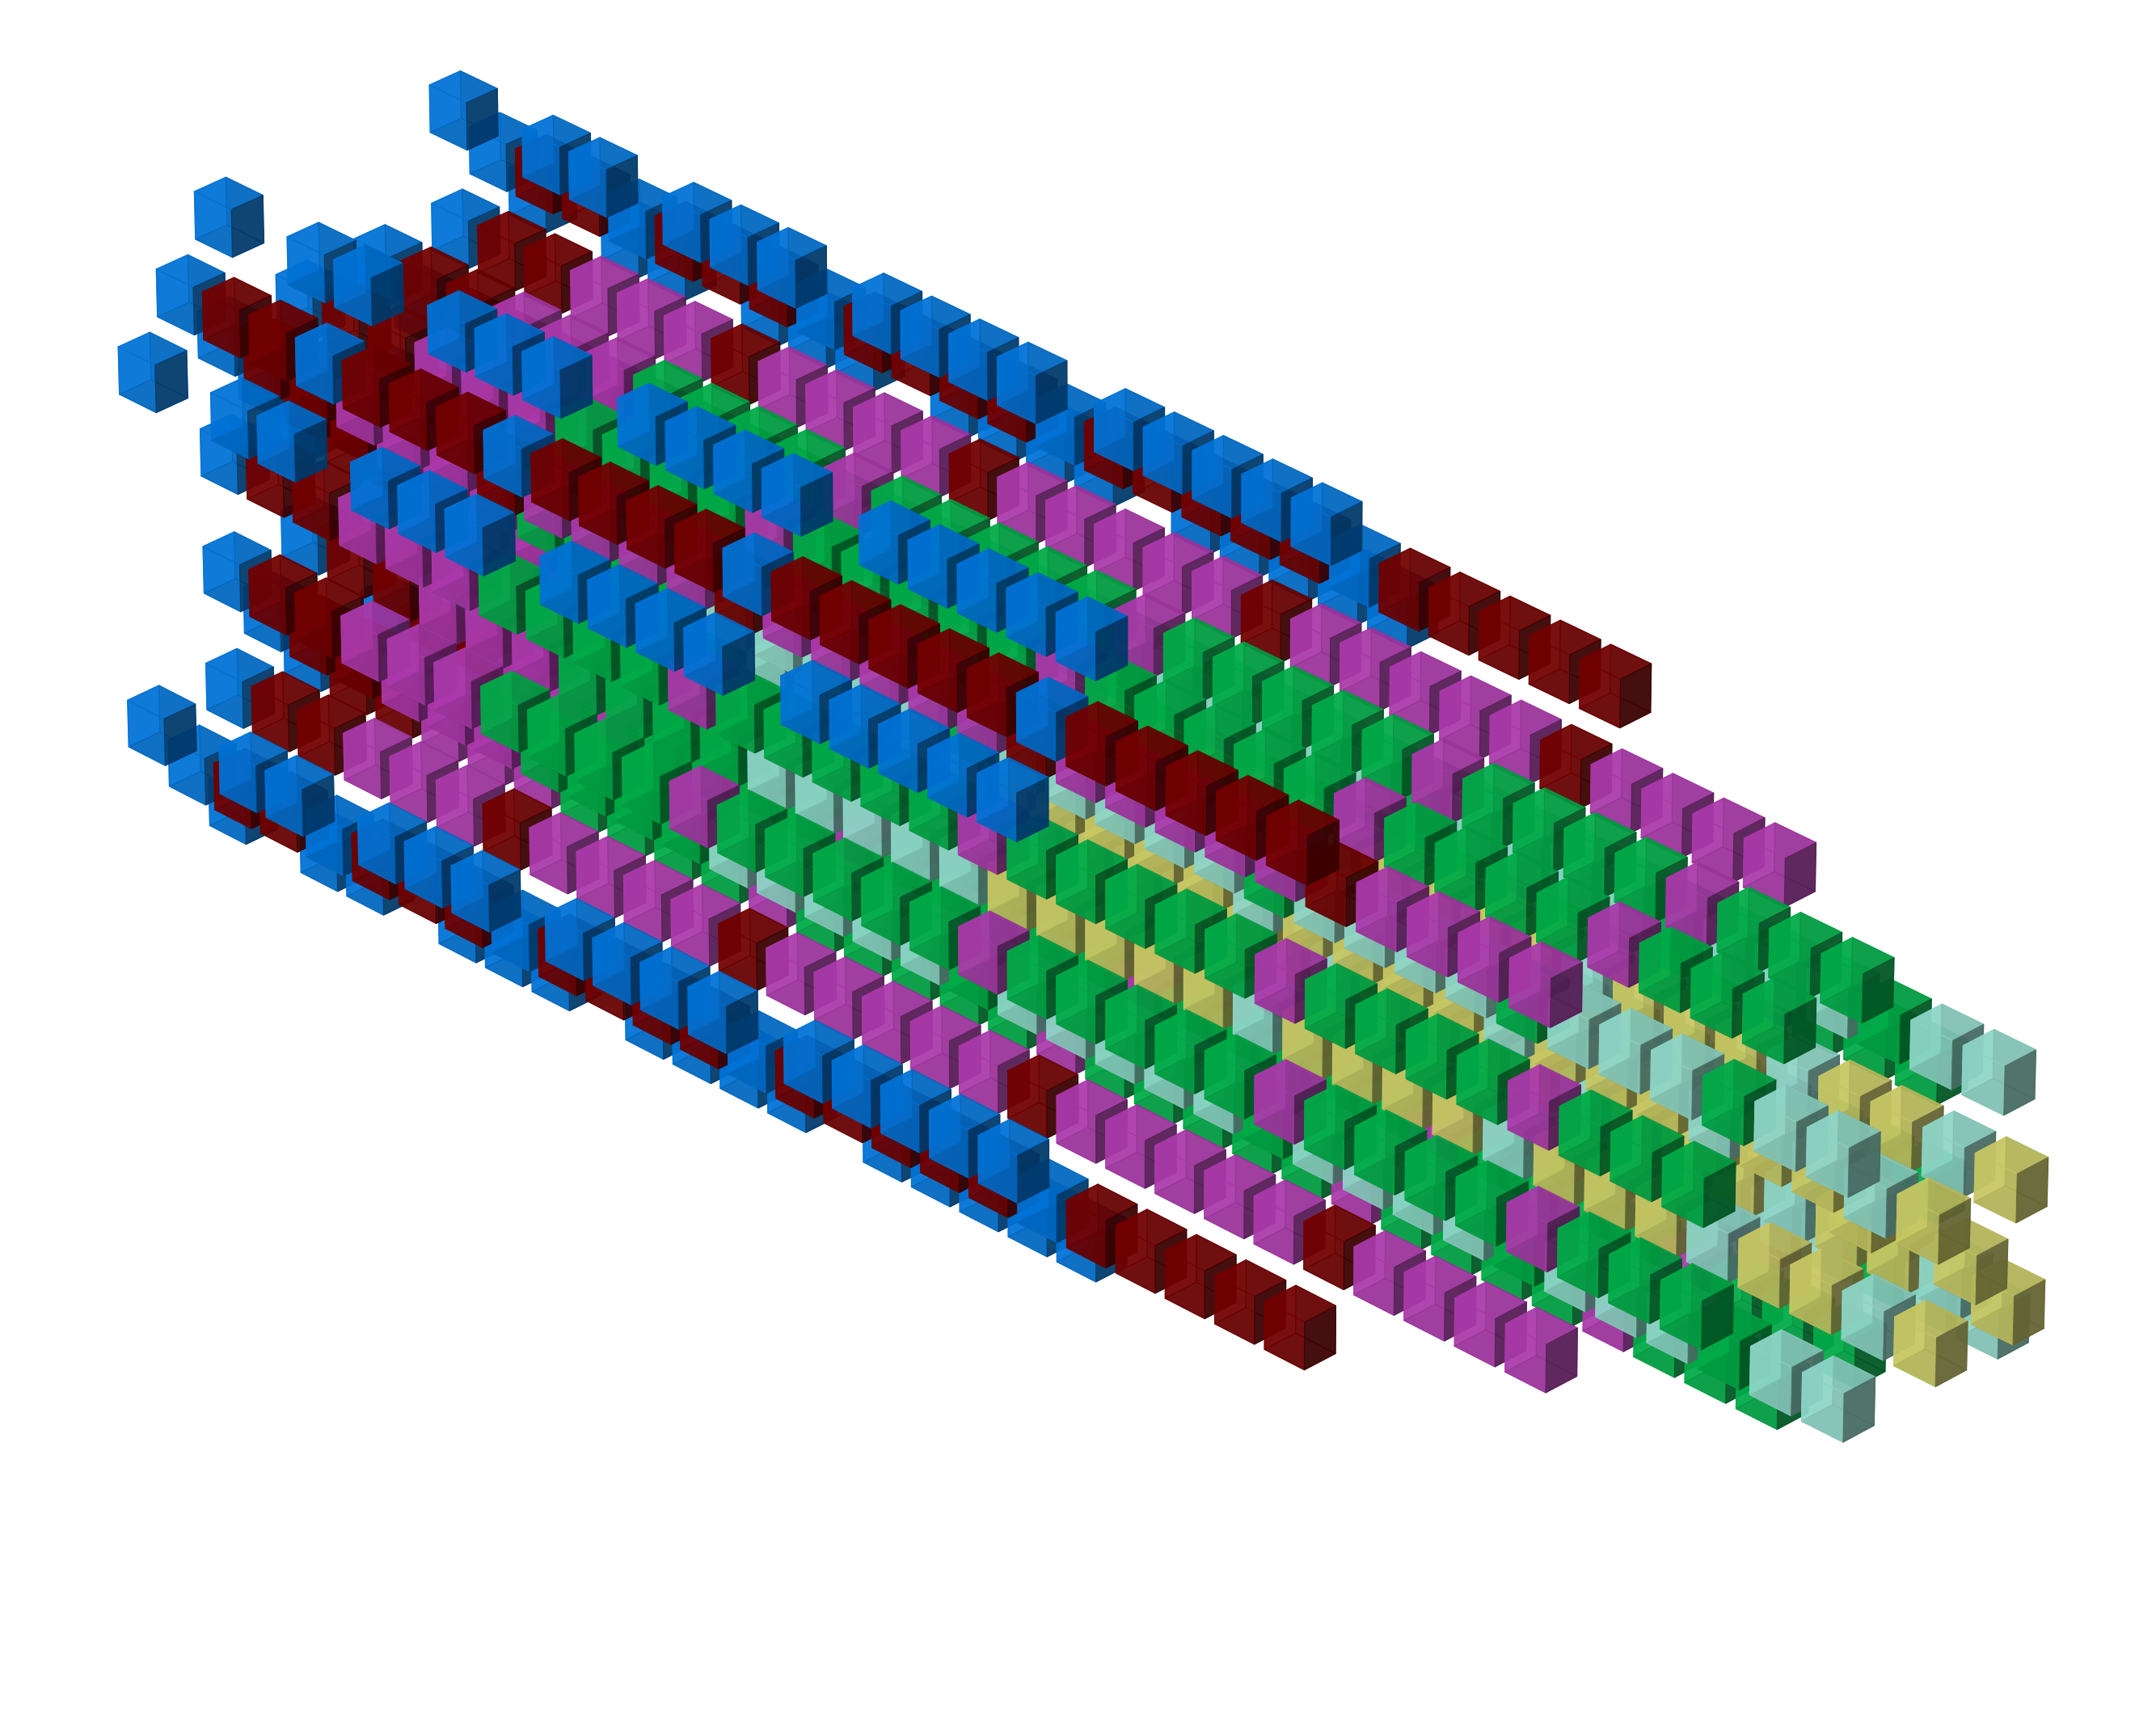
\includegraphics[width=12cm]{src/patterns/pattern6-225.png}%
    \end{adjustbox}
\caption{'Multi-Cross'.}
\end{figure}
\clearpage

\begin{lstlisting}
multicrossXPosArray 
        .BYTE $01,$01,$FF,$FF,$55                    ;
        .BYTE $02,$02,$FE,$FE,$55                    ;   5     5  
        .BYTE $01,$03,$03,$01,$FF,$FD,$FD,$FF,$55    ;  4       4 
        .BYTE $03,$03,$FD,$FD,$55                    ; 5 3 2 2 3 5
        .BYTE $04,$04,$FC,$FC,$55                    ;    1   1   
        .BYTE $03,$05,$05,$03,$FD,$FB,$FB,$FD,$55    ;   2 0 0 2  
        .BYTE $00,$55                                ;      6     
multicrossYPosArray                                  ;   2 0 0 2  
        .BYTE $FF,$01,$01,$FF,$55                    ;    1   1   
        .BYTE $FE,$02,$02,$FE,$55                    ; 5 3 2 2 3 5
        .BYTE $FD,$FF,$01,$03,$03,$01,$FF,$FD,$55    ;  4       4 
        .BYTE $FD,$03,$03,$FD,$55                    ;   5     5  
        .BYTE $FC,$04,$04,$FC,$55                    
        .BYTE $FB,$FD,$03,$05,$05,$03,$FD,$FB,$55    
        .BYTE $00,$55
\end{lstlisting}
\subfile{patterns/tables/pattern6.tex}

\begin{figure}[H]
    \centering
    \begin{adjustbox}{width=12cm,center}
      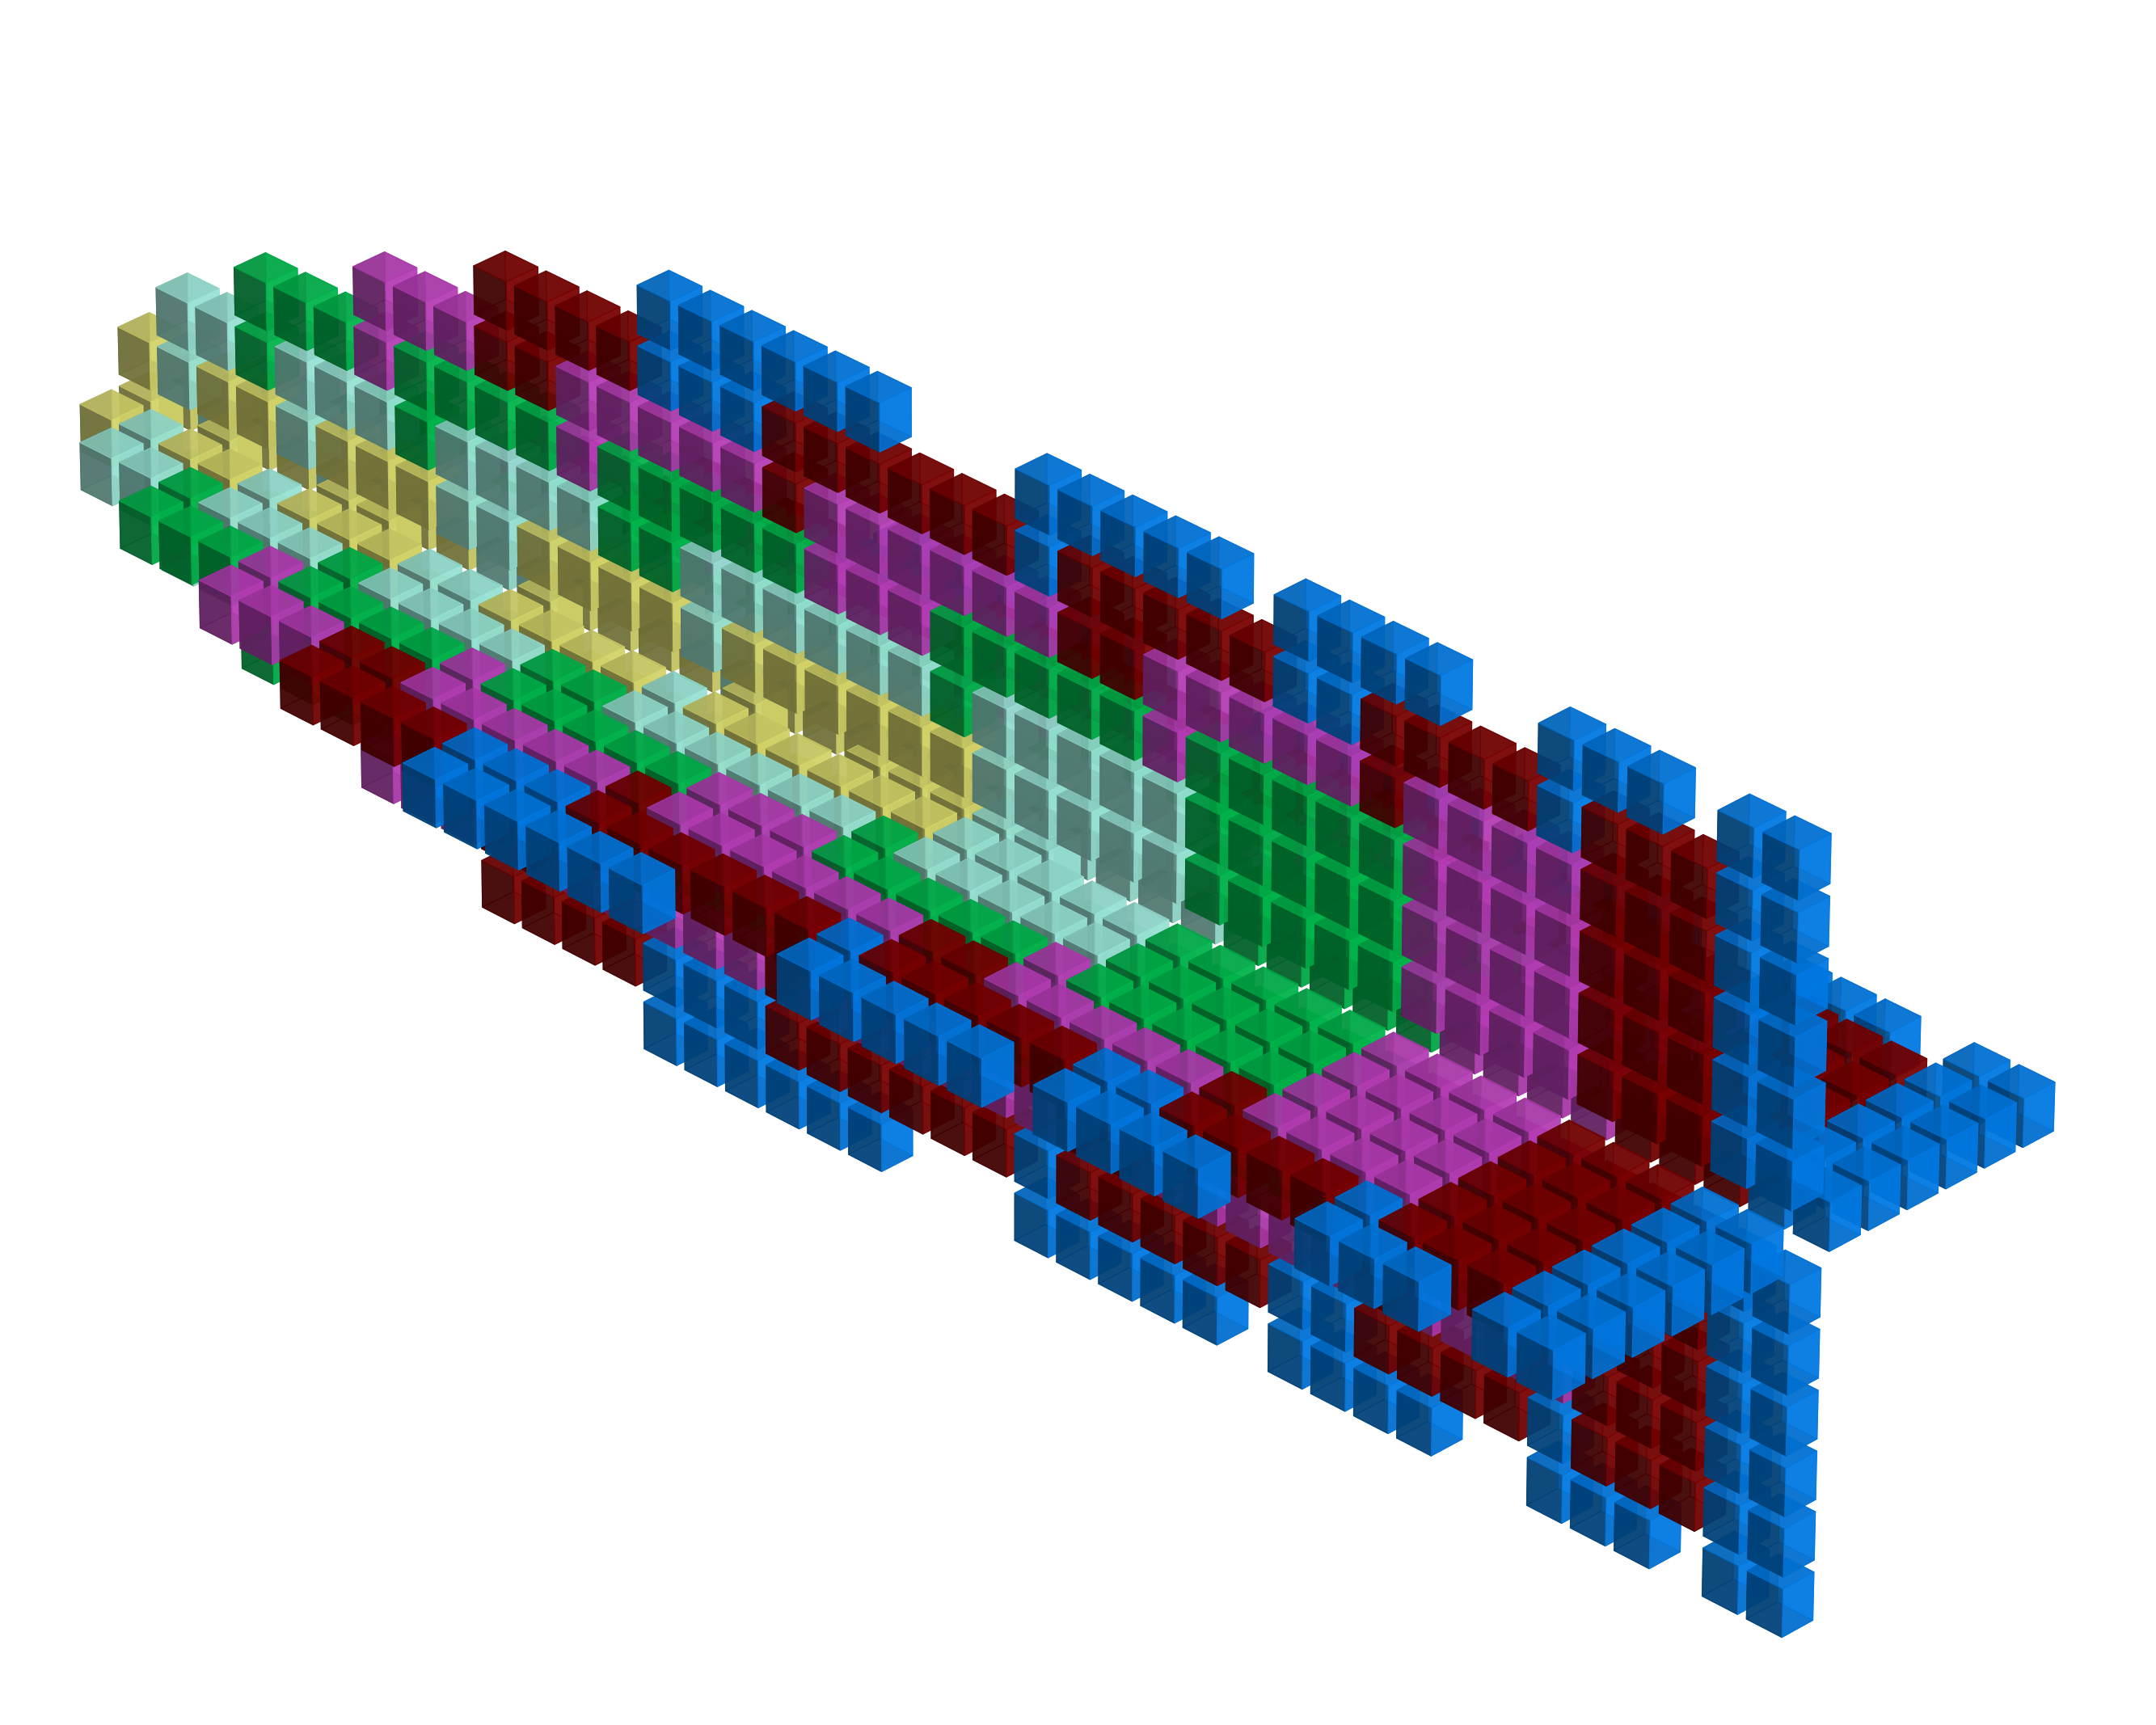
\includegraphics[width=12cm]{src/patterns/pattern7-45.png}%
    \end{adjustbox}
    \begin{adjustbox}{width=12cm,margin=0cm -4cm}
      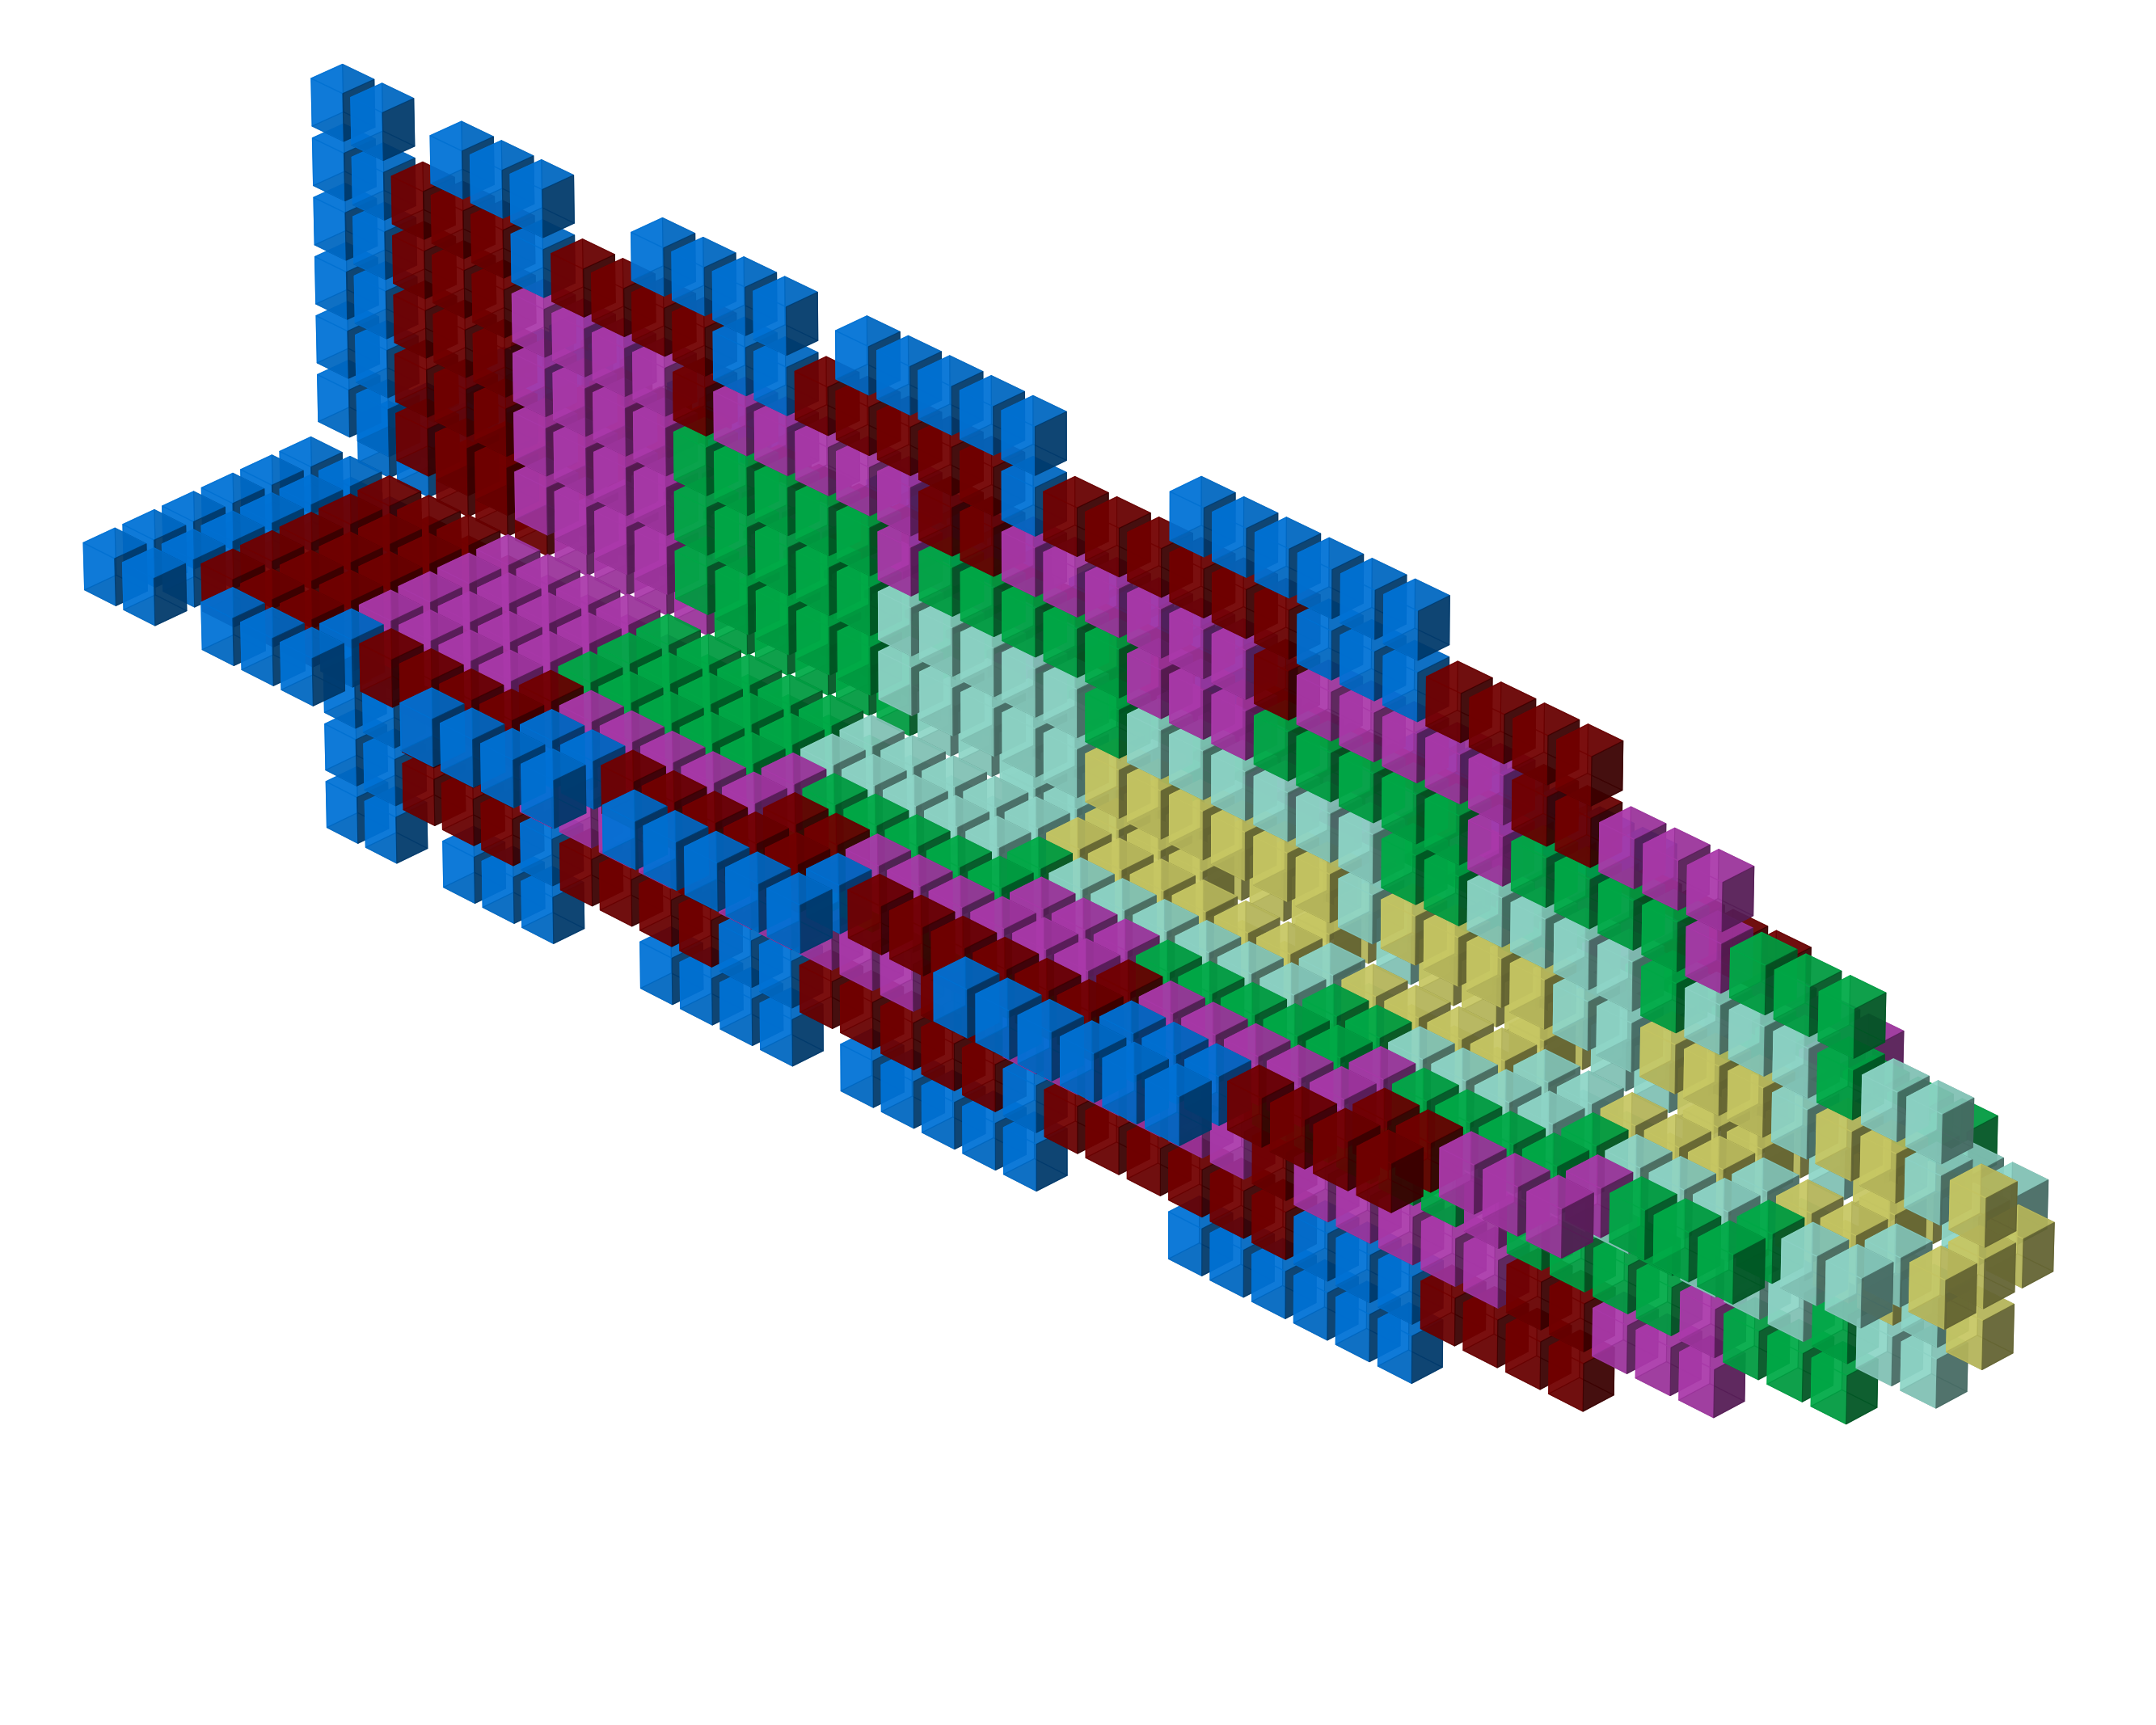
\includegraphics[width=12cm]{src/patterns/pattern7-225.png}%
    \end{adjustbox}
\caption{'Pulsar'.}
\end{figure}
\clearpage

\begin{lstlisting}
pulsarXPosArray .BYTE $00,$01,$00,$FF,$55       ;
                .BYTE $00,$02,$00,$FE,$55       ;       5      
                .BYTE $00,$03,$00,$FD,$55       ;       4      
                .BYTE $00,$04,$00,$FC,$55       ;       3      
                .BYTE $00,$05,$00,$FB,$55       ;       2      
                .BYTE $00,$06,$00,$FA,$55       ;       1      
                .BYTE $00,$55                   ;       0      
pulsarYPosArray .BYTE $FF,$00,$01,$00,$55       ; 5432106012345
                .BYTE $FE,$00,$02,$00,$55       ;       0      
                .BYTE $FD,$00,$03,$00,$55       ;       1      
                .BYTE $FC,$00,$04,$00,$55       ;       2      
                .BYTE $FB,$00,$05,$00,$55       ;       3      
                .BYTE $FA,$00,$06,$00,$55       ;       4      
                .BYTE $00,$55                   ;       5      
\end{lstlisting}
\subfile{patterns/tables/pattern7.tex}

\begin{figure}[H]
    \centering
    \begin{adjustbox}{width=12cm,center}
      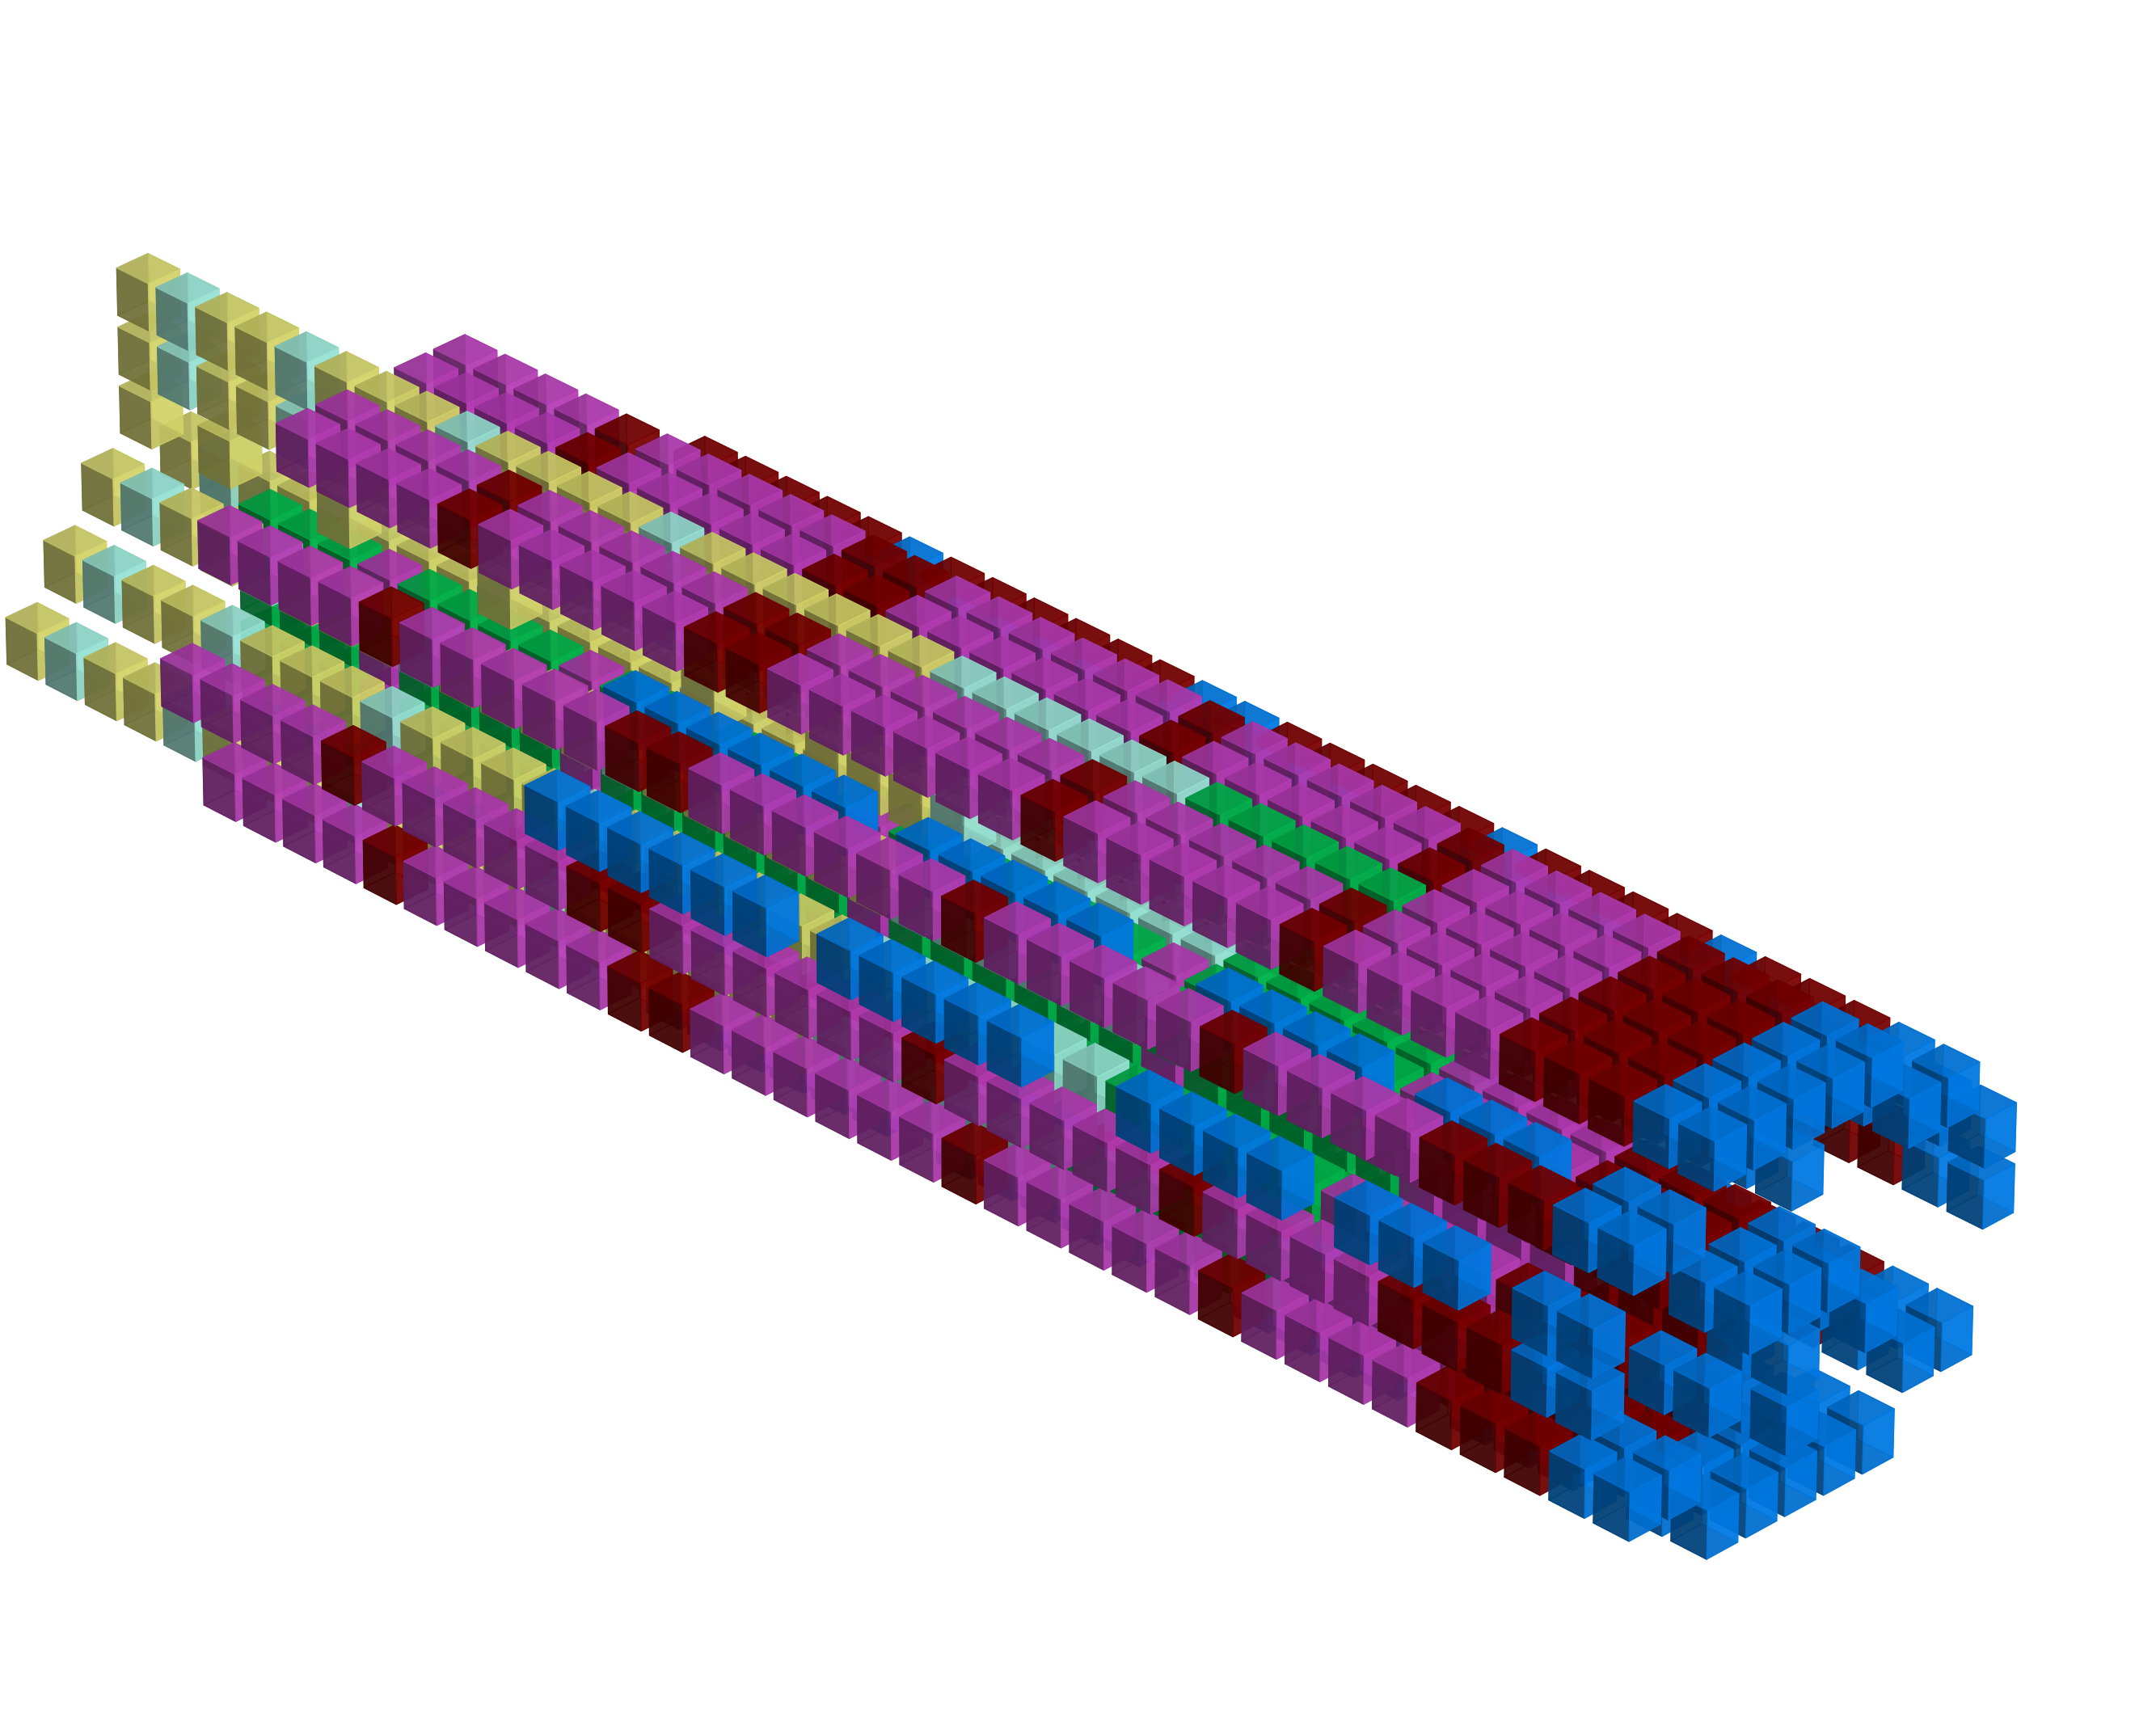
\includegraphics[width=12cm]{src/patterns/pattern8-45.png}%
    \end{adjustbox}
    \begin{adjustbox}{width=12cm,margin=0cm -4cm}
      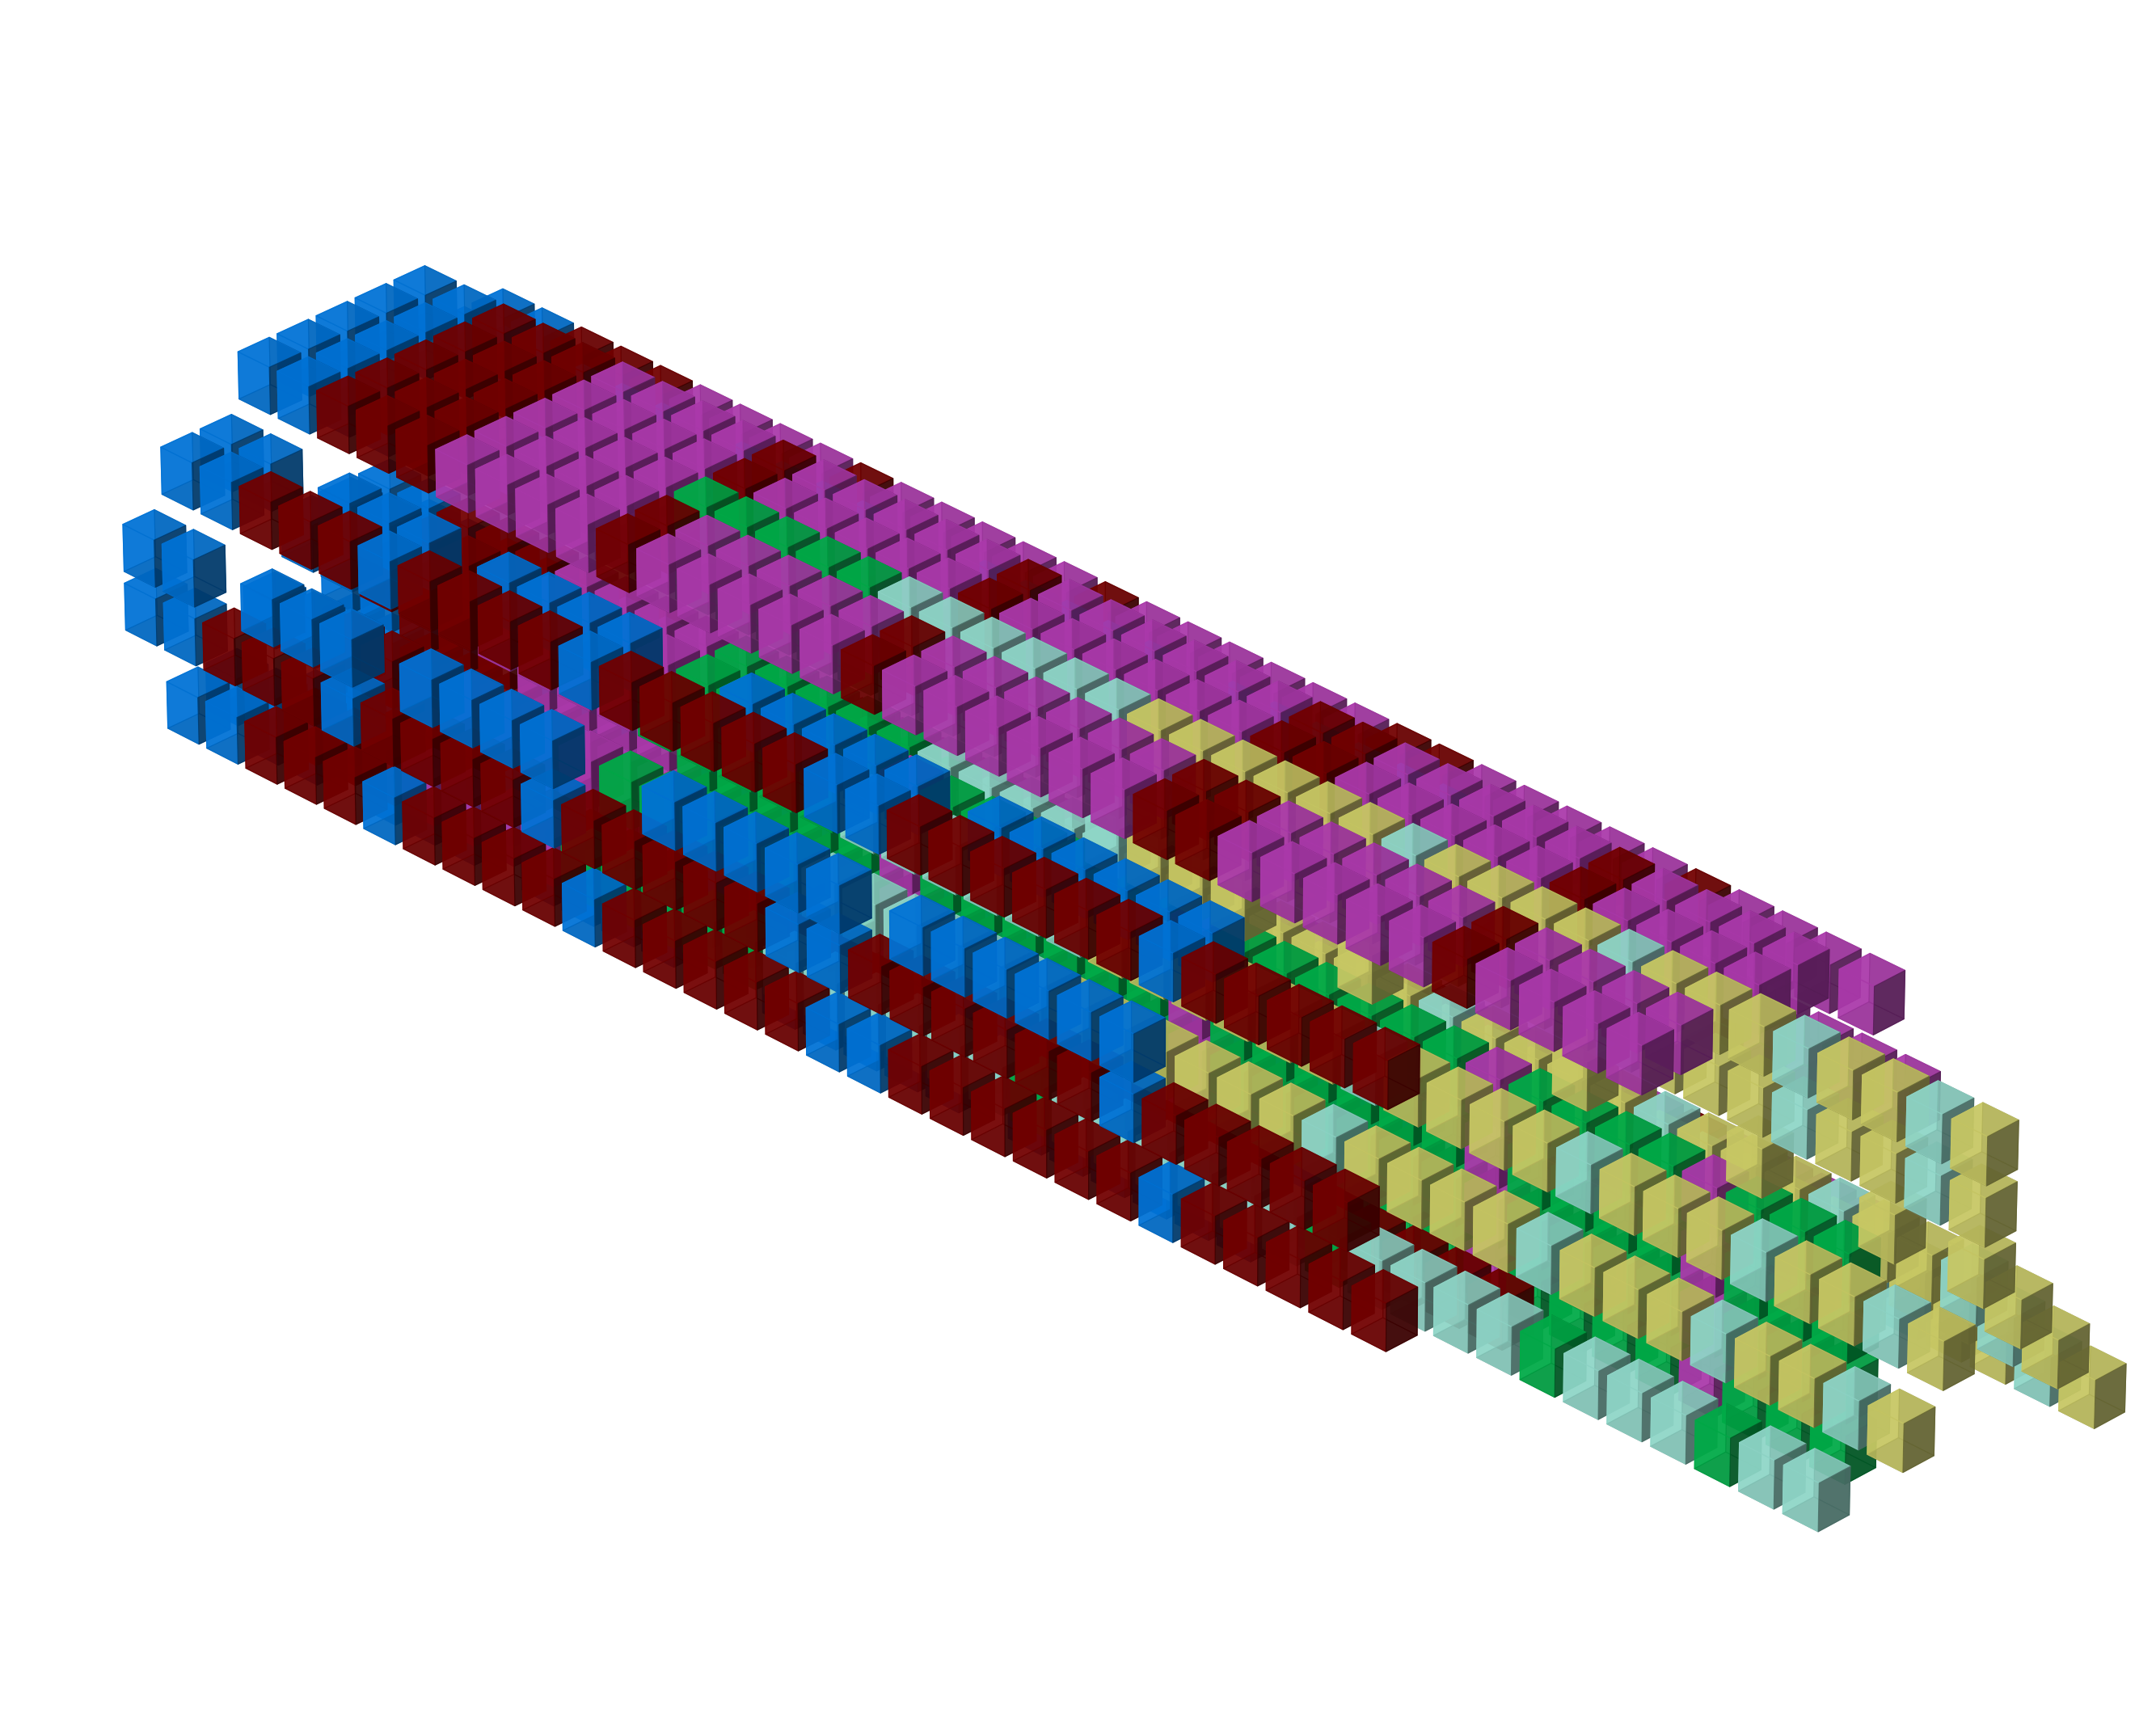
\includegraphics[width=12cm]{src/patterns/pattern8-225.png}%
    \end{adjustbox}
\caption{'Custom Pattern 1'.}
\end{figure}
\clearpage

\begin{lstlisting}
; customPattern0XPosArray                         ;
        .BYTE $00,$00,$00,$FF,$FE,$FD,$01,$02,$55 ;    33033   
        .BYTE $00,$03,$55                         ;  35  0  54 
        .BYTE $00,$00,$00,$00,$00,$55             ; 5    6    5
        .BYTE $00,$FF,$FE,$FC,$FB,$FC,$01,$02,$55 ; 3   020   4
        .BYTE $00,$04,$05,$04,$FF,$01,$55         ;    0 2 0   
        .BYTE $00,$FD,$FB,$03,$05,$02,$FE,$55     ;  30  2  14 
        .BYTE $00,$55                             ;    54245   
; customPattern0YPosArray
        .BYTE $00,$FF,$FE,$01,$02,$03,$01,$02,$55
        .BYTE $00,$03,$55
        .BYTE $00,$01,$02,$03,$04,$55
        .BYTE $00,$FE,$FE,$FF,$01,$03,$FE,$FE,$55
        .BYTE $00,$FF,$01,$03,$04,$04,$55
        .BYTE $00,$FF,$00,$FF,$00,$04,$04,$55
        .BYTE $00,$55

\end{lstlisting}
\subfile{patterns/tables/pattern8.tex}

\begin{figure}[H]
    \centering
    \begin{adjustbox}{width=12cm,center}
      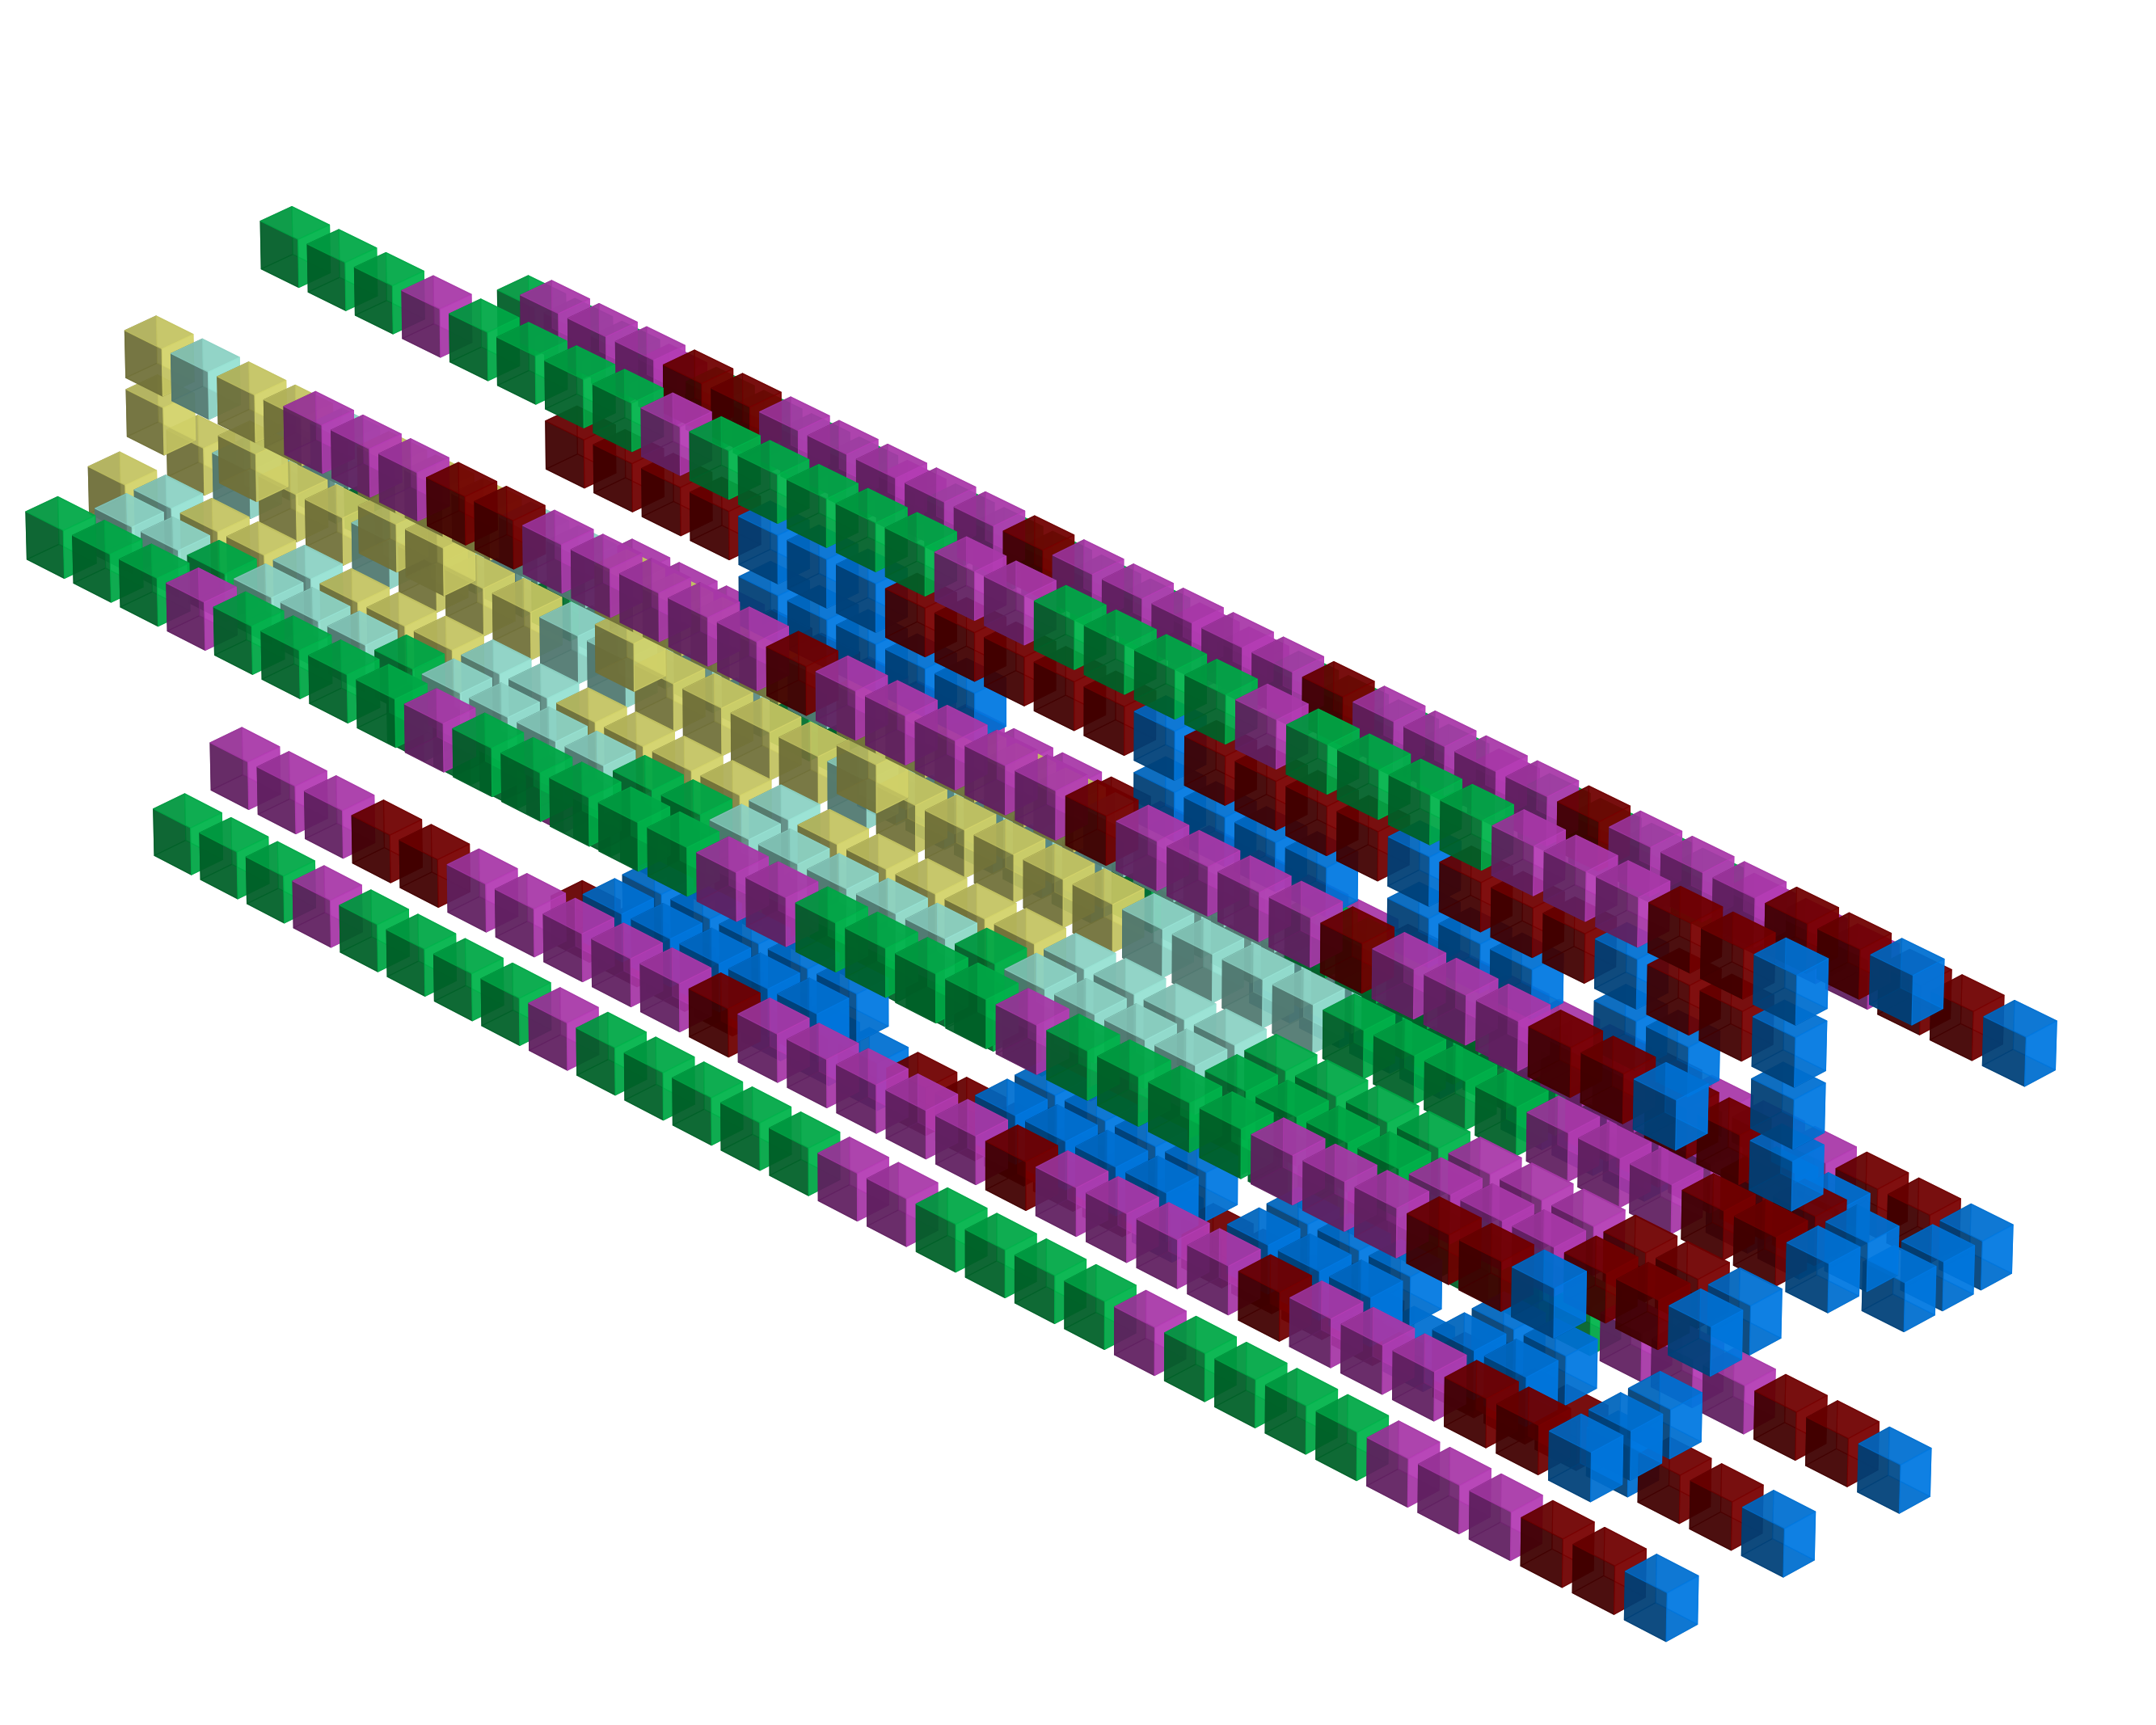
\includegraphics[width=12cm]{src/patterns/pattern9-45.png}%
    \end{adjustbox}
    \begin{adjustbox}{width=12cm,margin=0cm -4cm}
      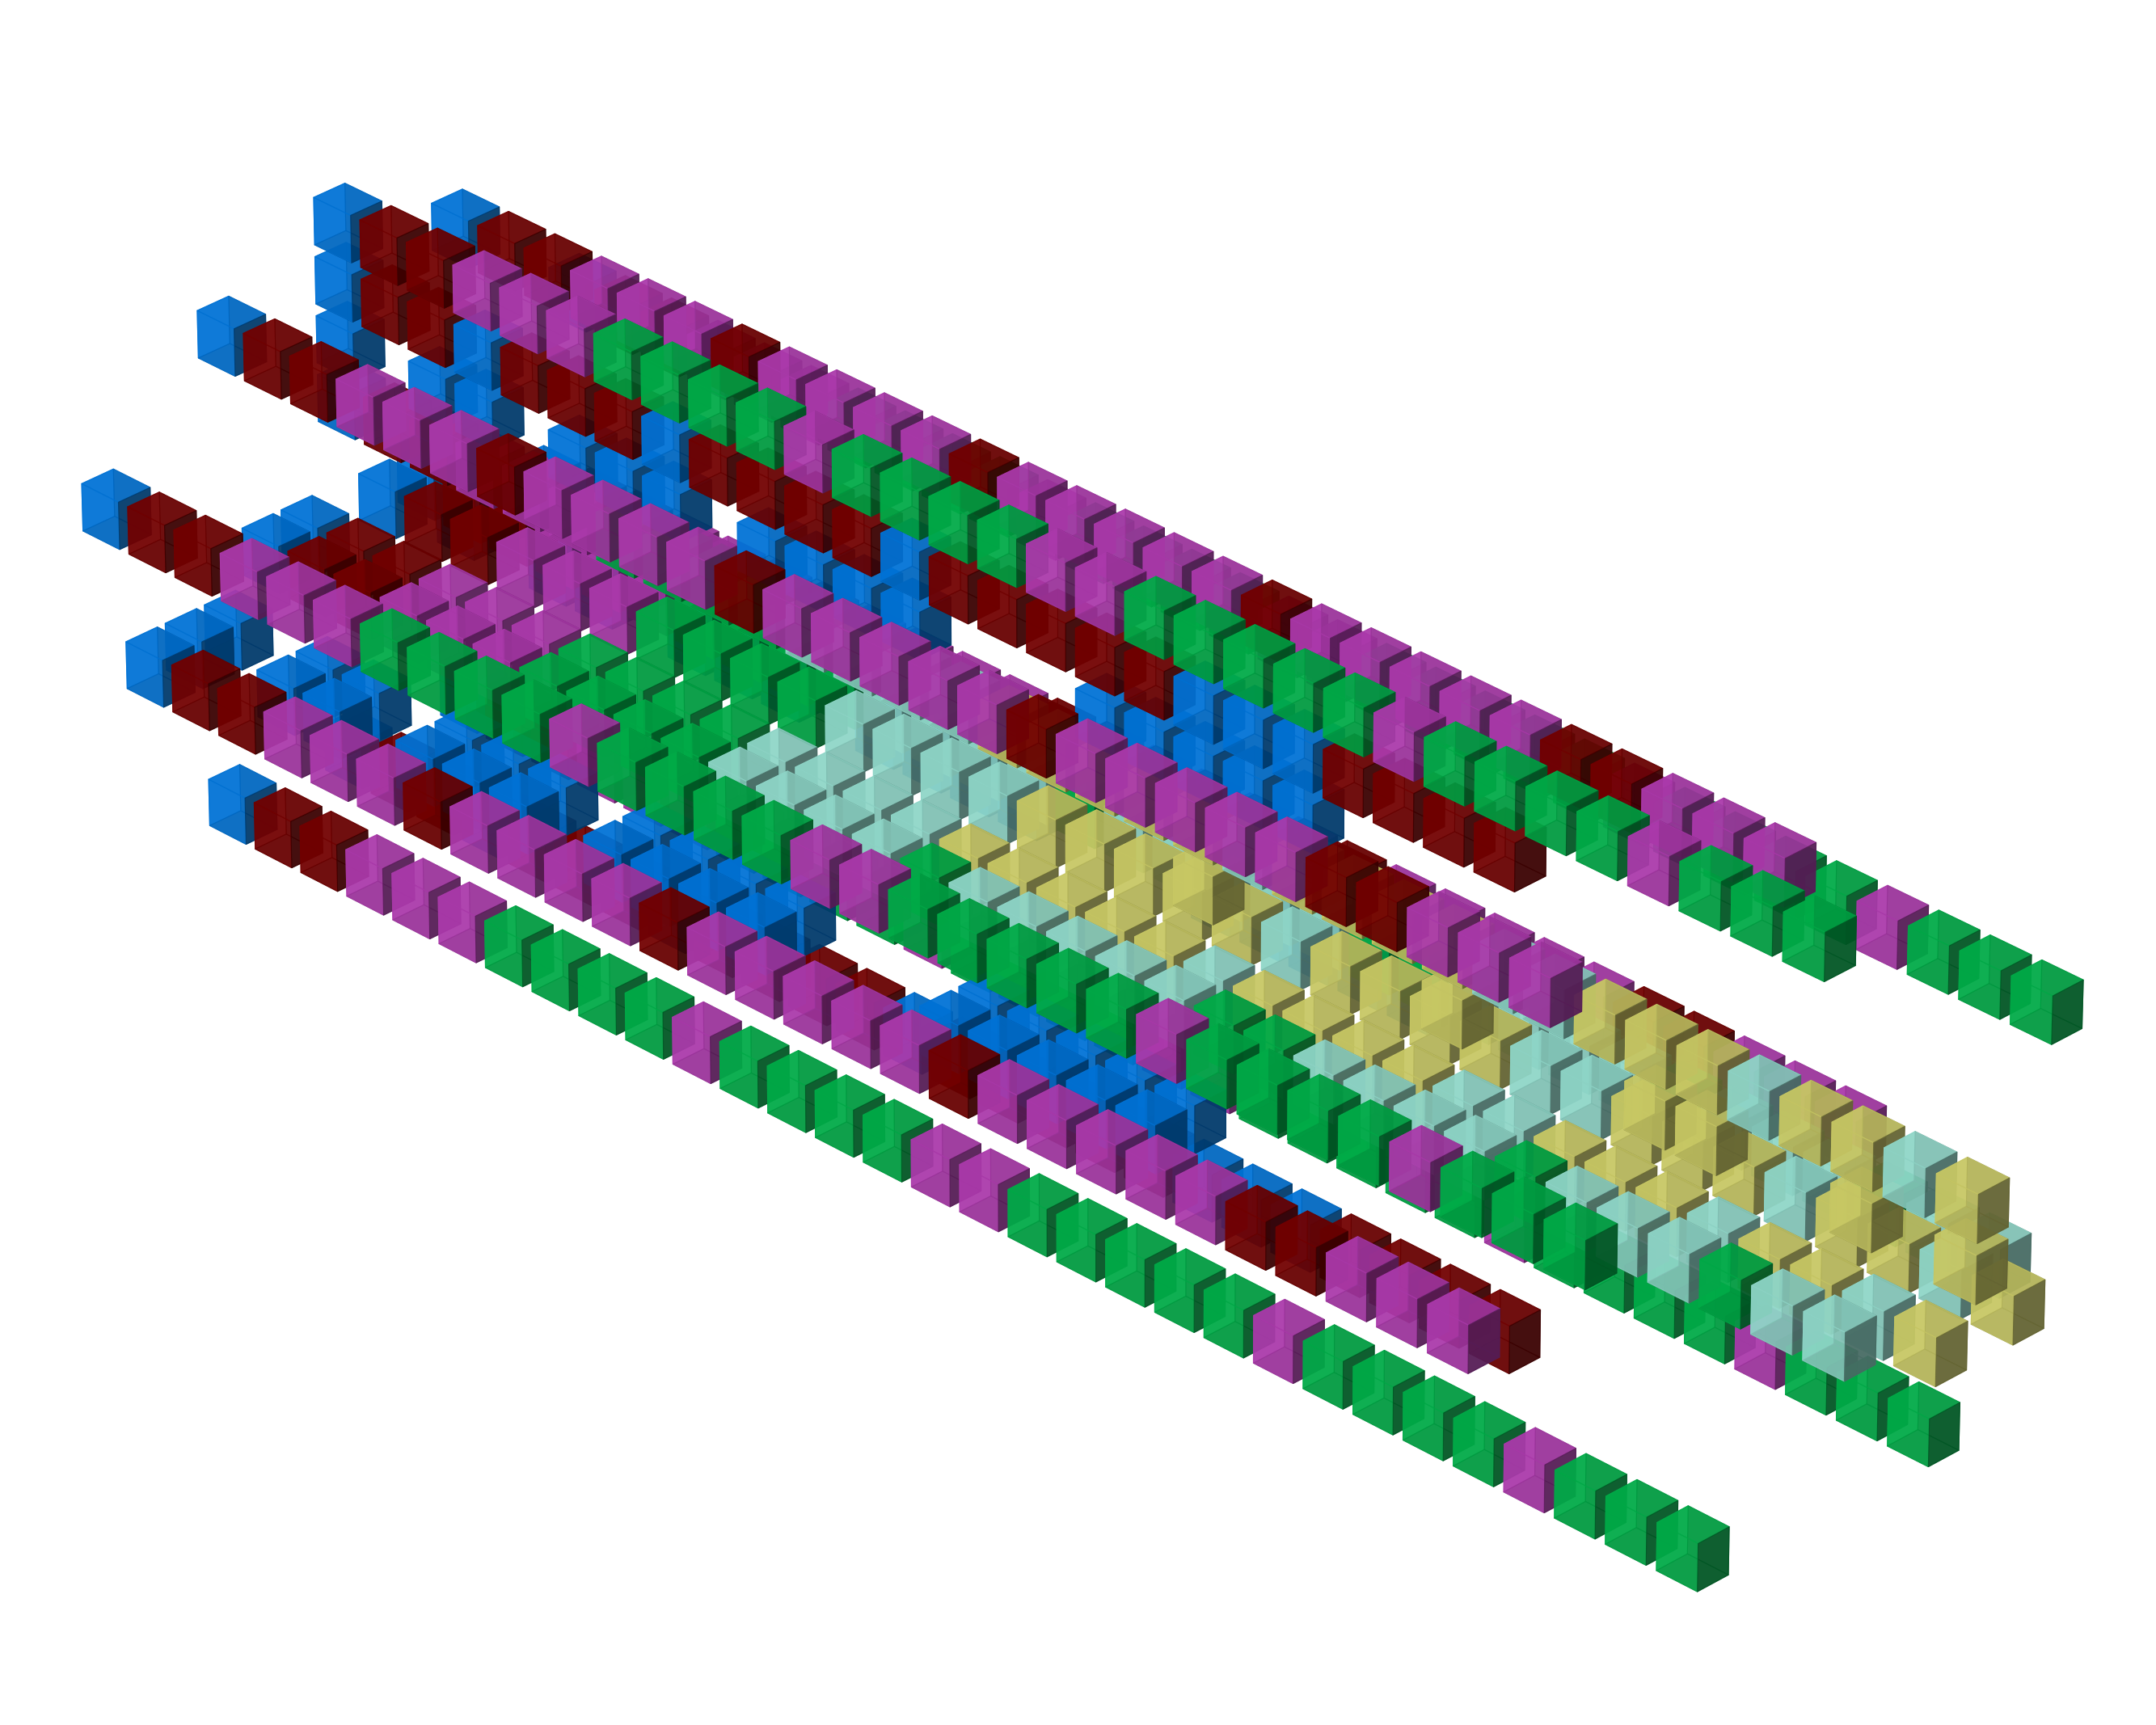
\includegraphics[width=12cm]{src/patterns/pattern9-225.png}%
    \end{adjustbox}
\caption{'Custom Pattern 2'.}
\end{figure}
\clearpage

\begin{lstlisting}
; customPattern1XPosArray                   ;       3      
        .BYTE $00,$00,$FF,$01,$55           ;    4  5  4   
        .BYTE $00,$FE,$02,$55               ;       6      
        .BYTE $00,$00,$FA,$06,$03,$FD,$55   ; 3     1     3
        .BYTE $00,$FD,$03,$FB,$05,$55       ;       7      
        .BYTE $00,$00,$00,$55               ;     21 12    
        .BYTE $00,$00,$FC,$04,$03,$FD,$55   ;  466     664 
        .BYTE $00,$55                       ;              
; customPattern1YPosArray                   ;    3  5  3   
        .BYTE $00,$FF,$01,$01,$55
        .BYTE $00,$01,$01,$55
        .BYTE $00,$FC,$FF,$FF,$05,$05,$55
        .BYTE $00,$FD,$FD,$02,$02,$55
        .BYTE $00,$05,$FD,$55
        .BYTE $00,$FE,$02,$02,$02,$02,$55
        .BYTE $00,$55


\end{lstlisting}
\subfile{patterns/tables/pattern9.tex}

\begin{figure}[H]
    \centering
    \begin{adjustbox}{width=12cm,center}
      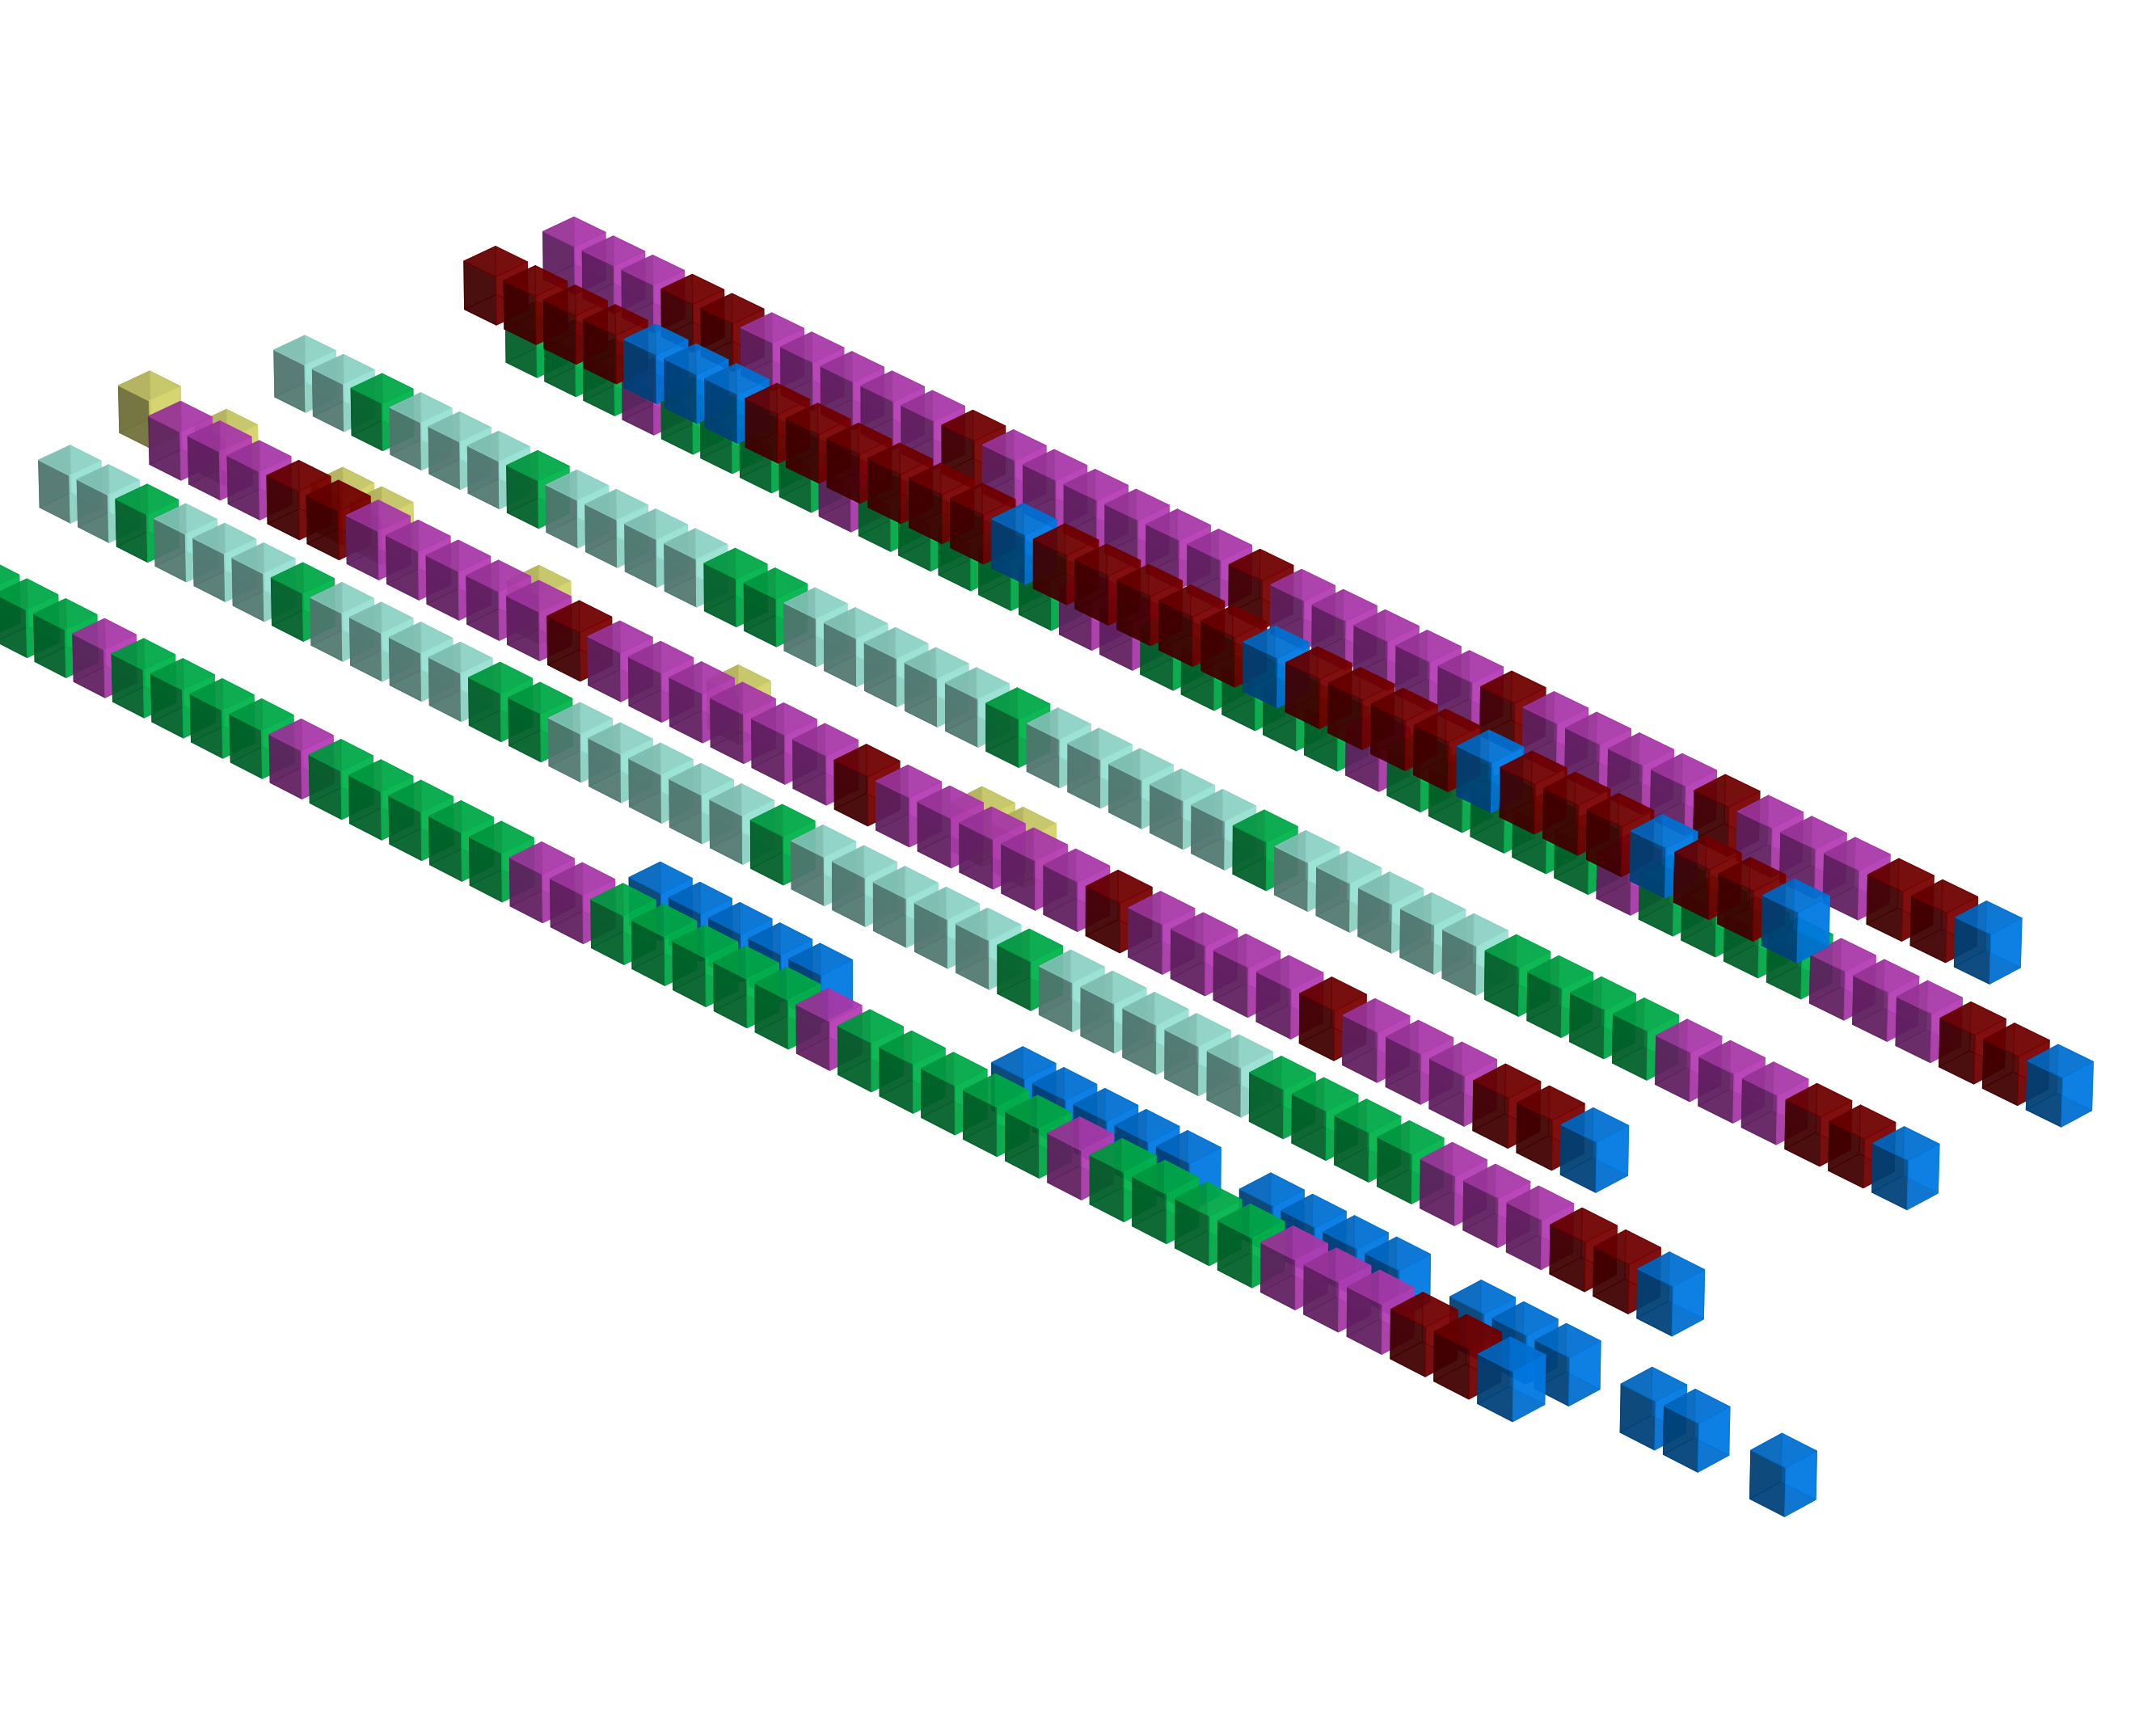
\includegraphics[width=12cm]{src/patterns/pattern10-45.png}%
    \end{adjustbox}
    \begin{adjustbox}{width=12cm,margin=0cm -4cm}
      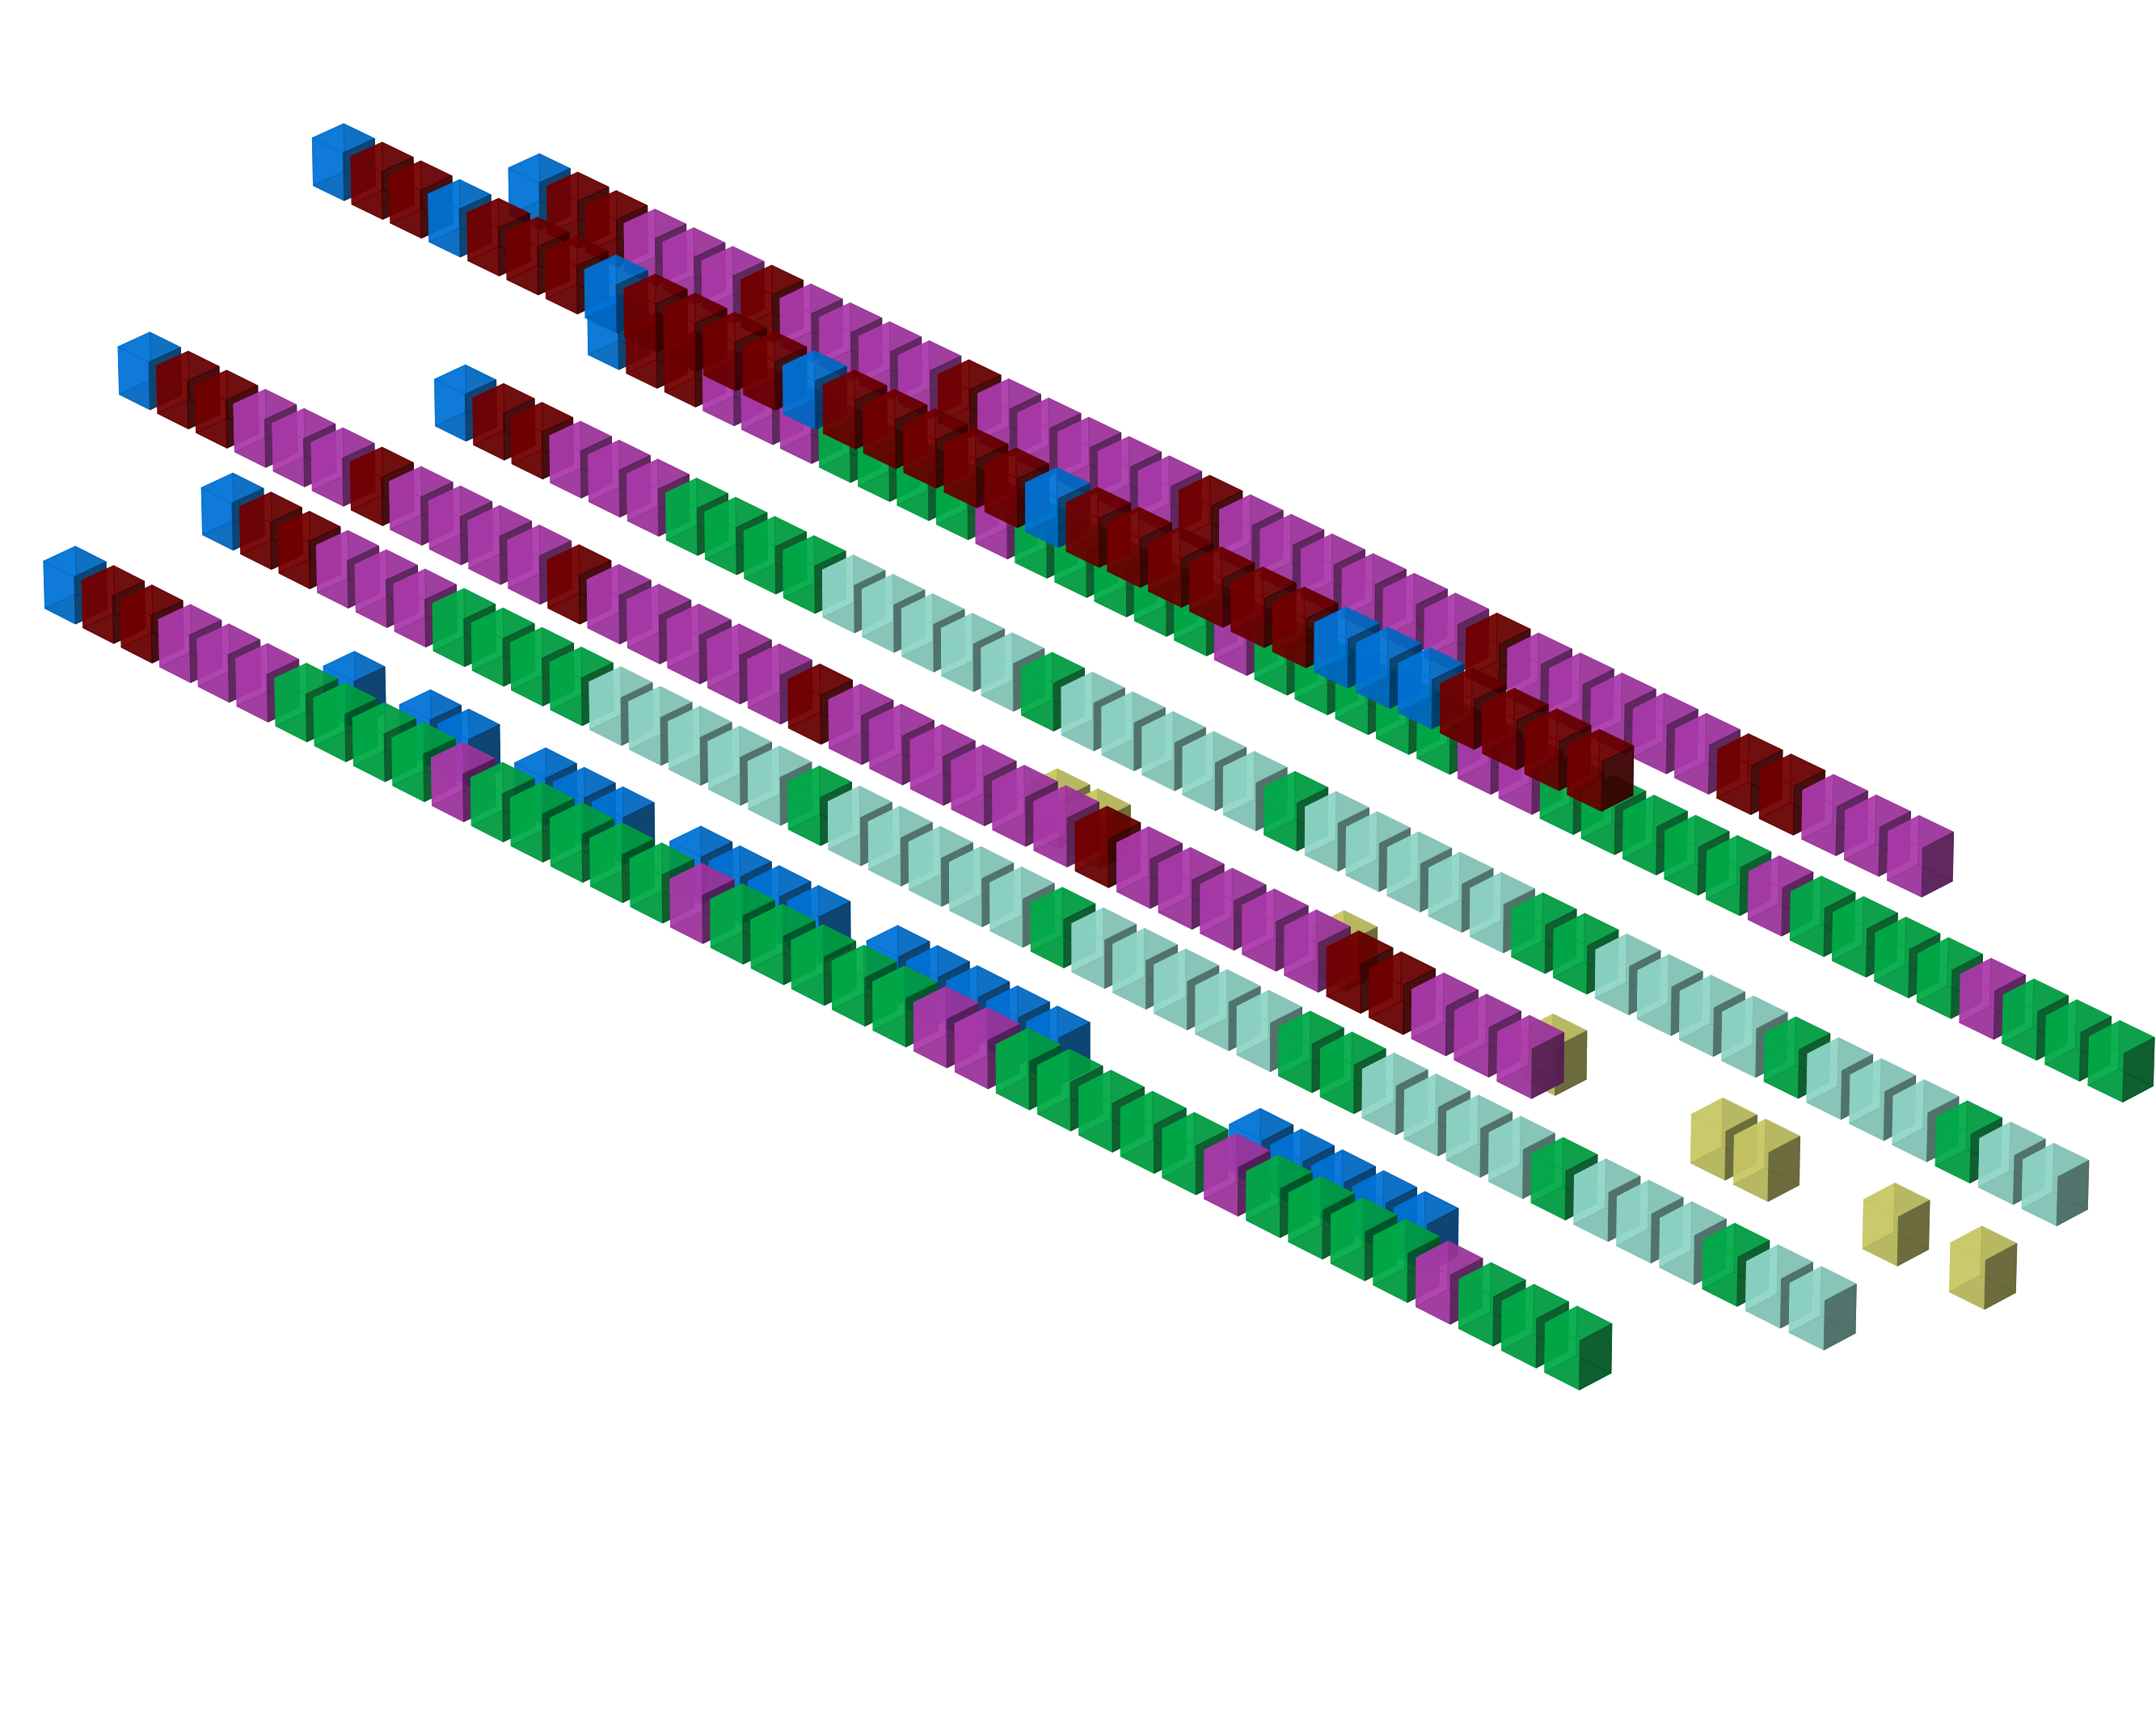
\includegraphics[width=12cm]{src/patterns/pattern10-225.png}%
    \end{adjustbox}
\caption{'Custom Pattern 3'.}
\end{figure}
\clearpage

\begin{lstlisting}
; customPattern2XPosArray      ;        5       
        .BYTE $00,$55          ;      8   8     
        .BYTE $00,$FD,$03,$55  ;   4         4  
        .BYTE $00,$F9,$07,$55  ;                
        .BYTE $00,$FB,$05,$55  ;                
        .BYTE $00,$00,$55      ; 3   2  9  2   3
        .BYTE $00,$00,$55      ;                
        .BYTE $00,$55          ;                
        .BYTE $FE,$02,$55      ;                
        .BYTE $00,$55          ;        6       
; customPattern2YPosArray
        .BYTE $00,$55
        .BYTE $00,$00,$00,$55
        .BYTE $00,$00,$00,$55
        .BYTE $00,$FD,$FD,$55
        .BYTE $00,$FB,$55
        .BYTE $00,$04,$55
        .BYTE $00,$55
        .BYTE $FC,$FC,$55
        .BYTE $00,$55
\end{lstlisting}
\subfile{patterns/tables/pattern10.tex}

\begin{figure}[H]
    \centering
    \begin{adjustbox}{width=12cm,center}
      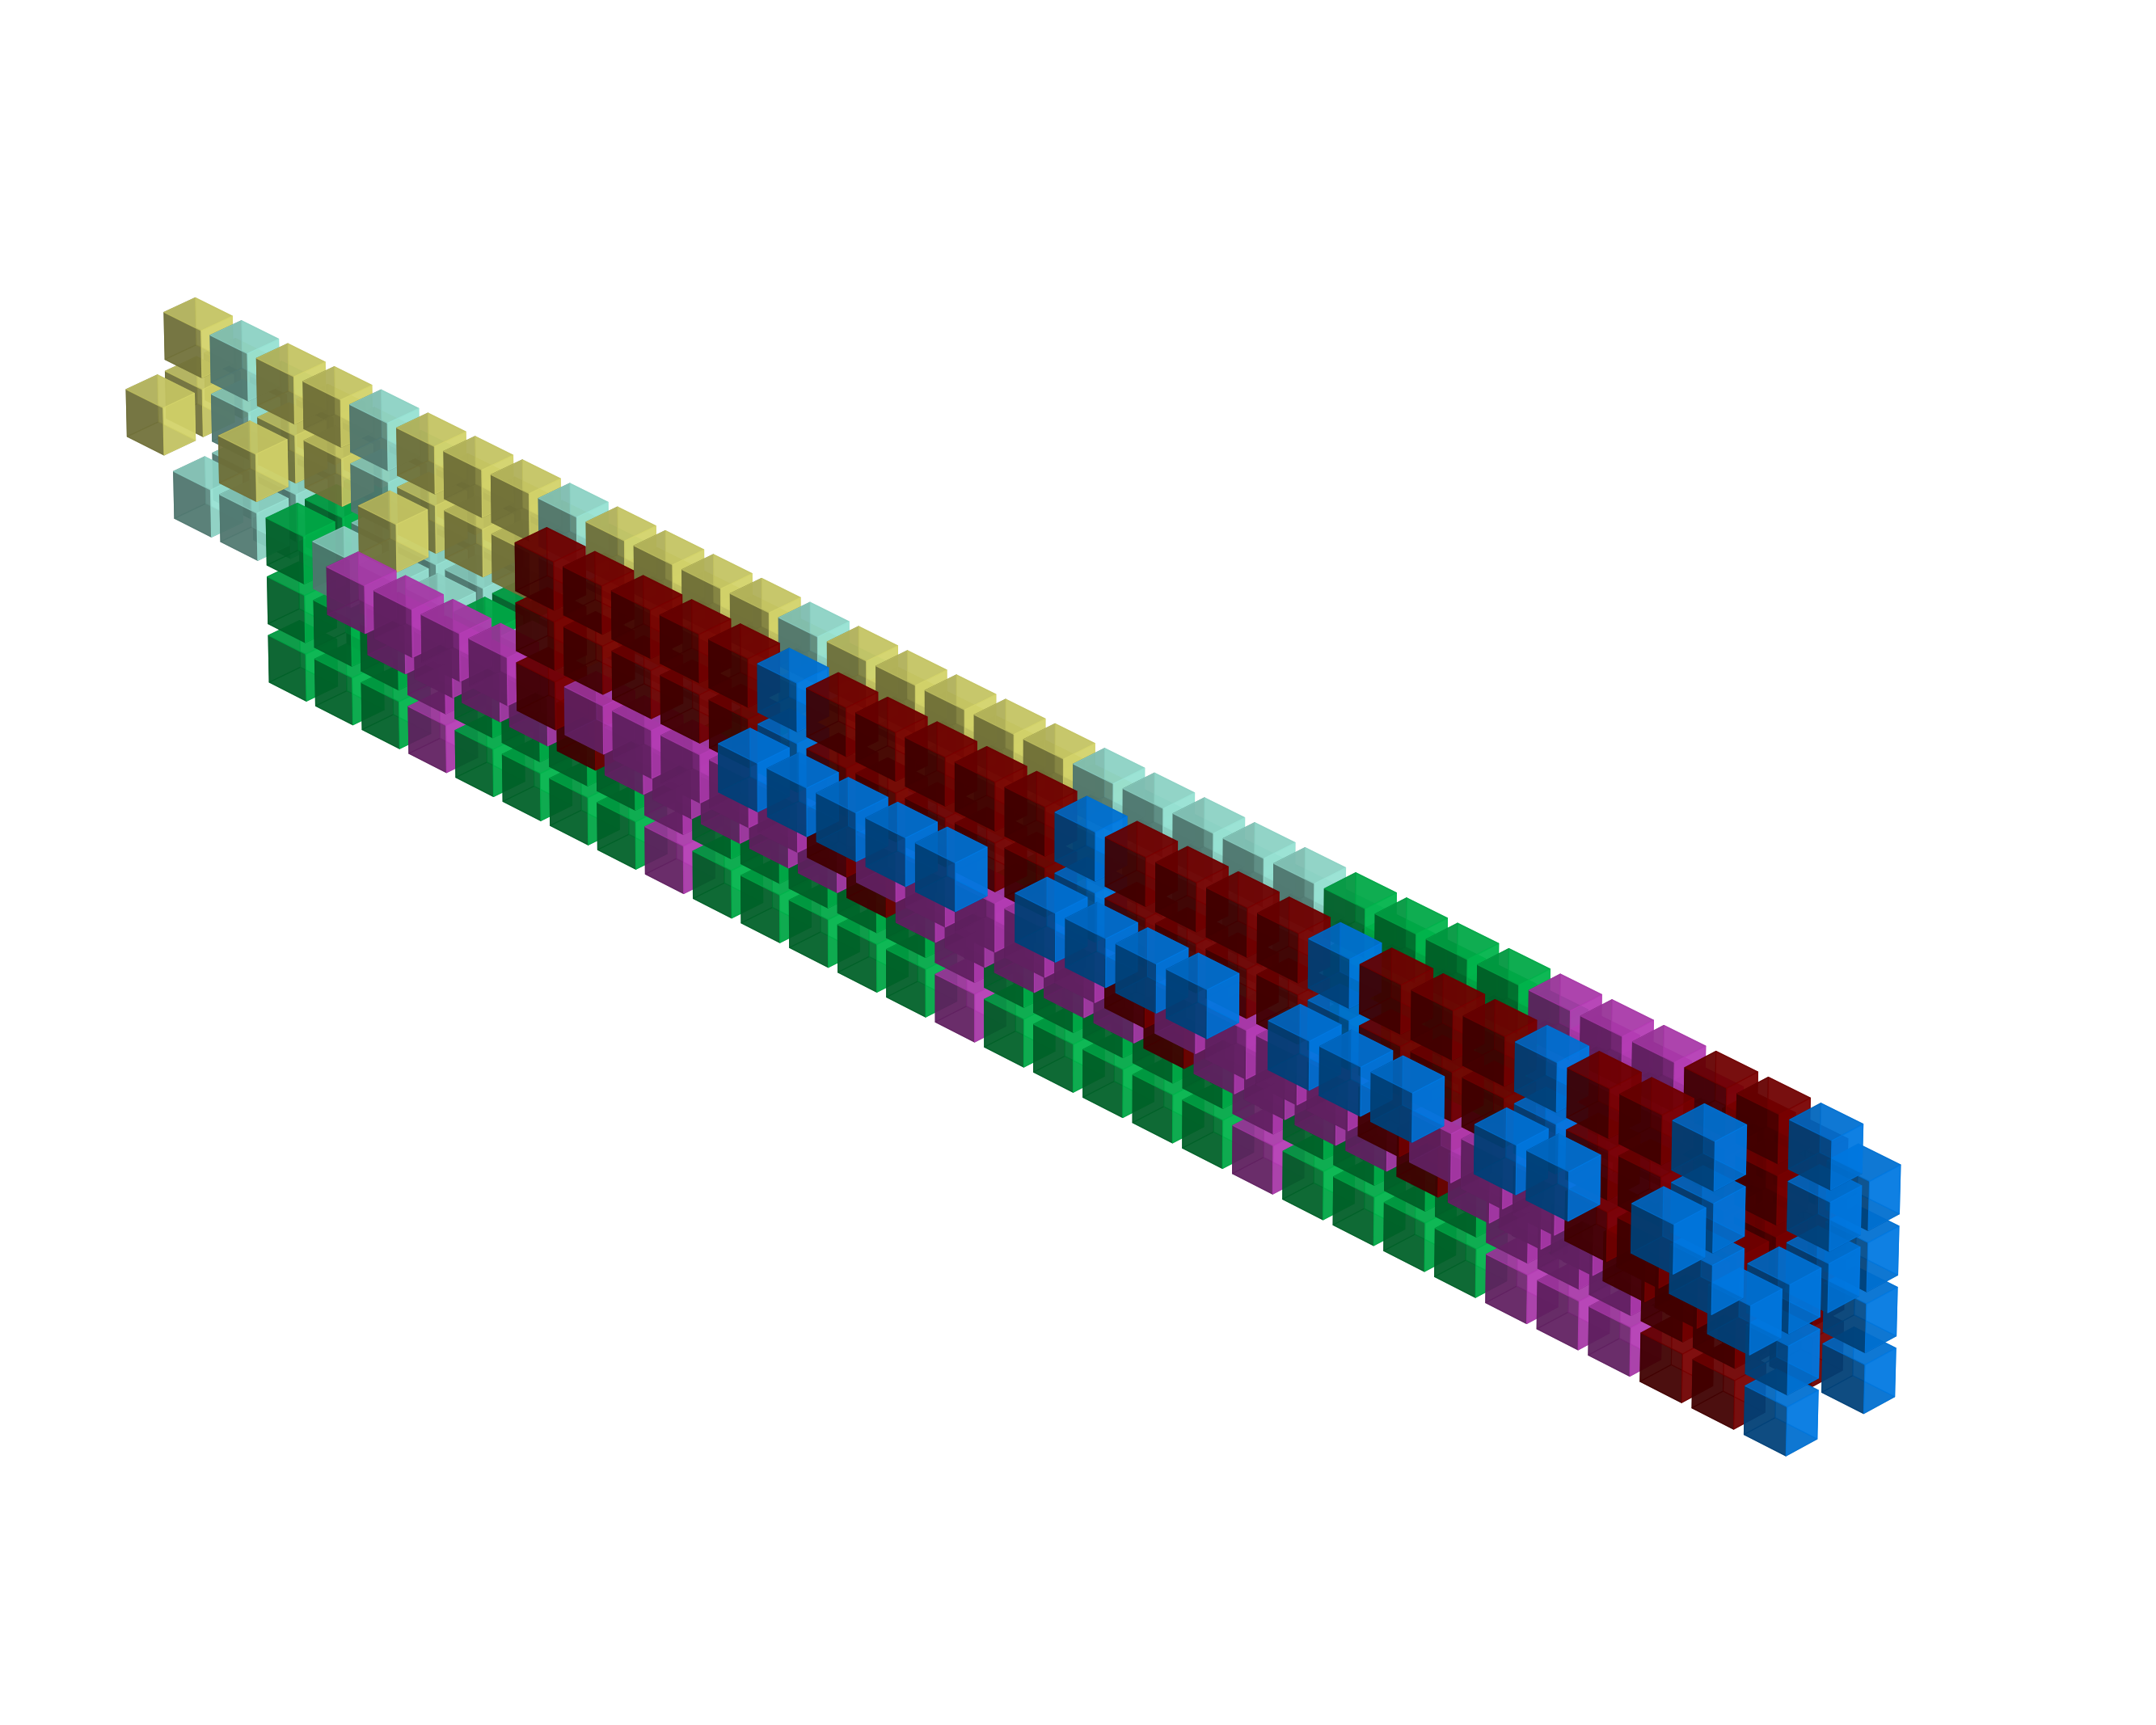
\includegraphics[width=12cm]{src/patterns/pattern11-45.png}%
    \end{adjustbox}
    \begin{adjustbox}{width=12cm,margin=0cm -4cm}
      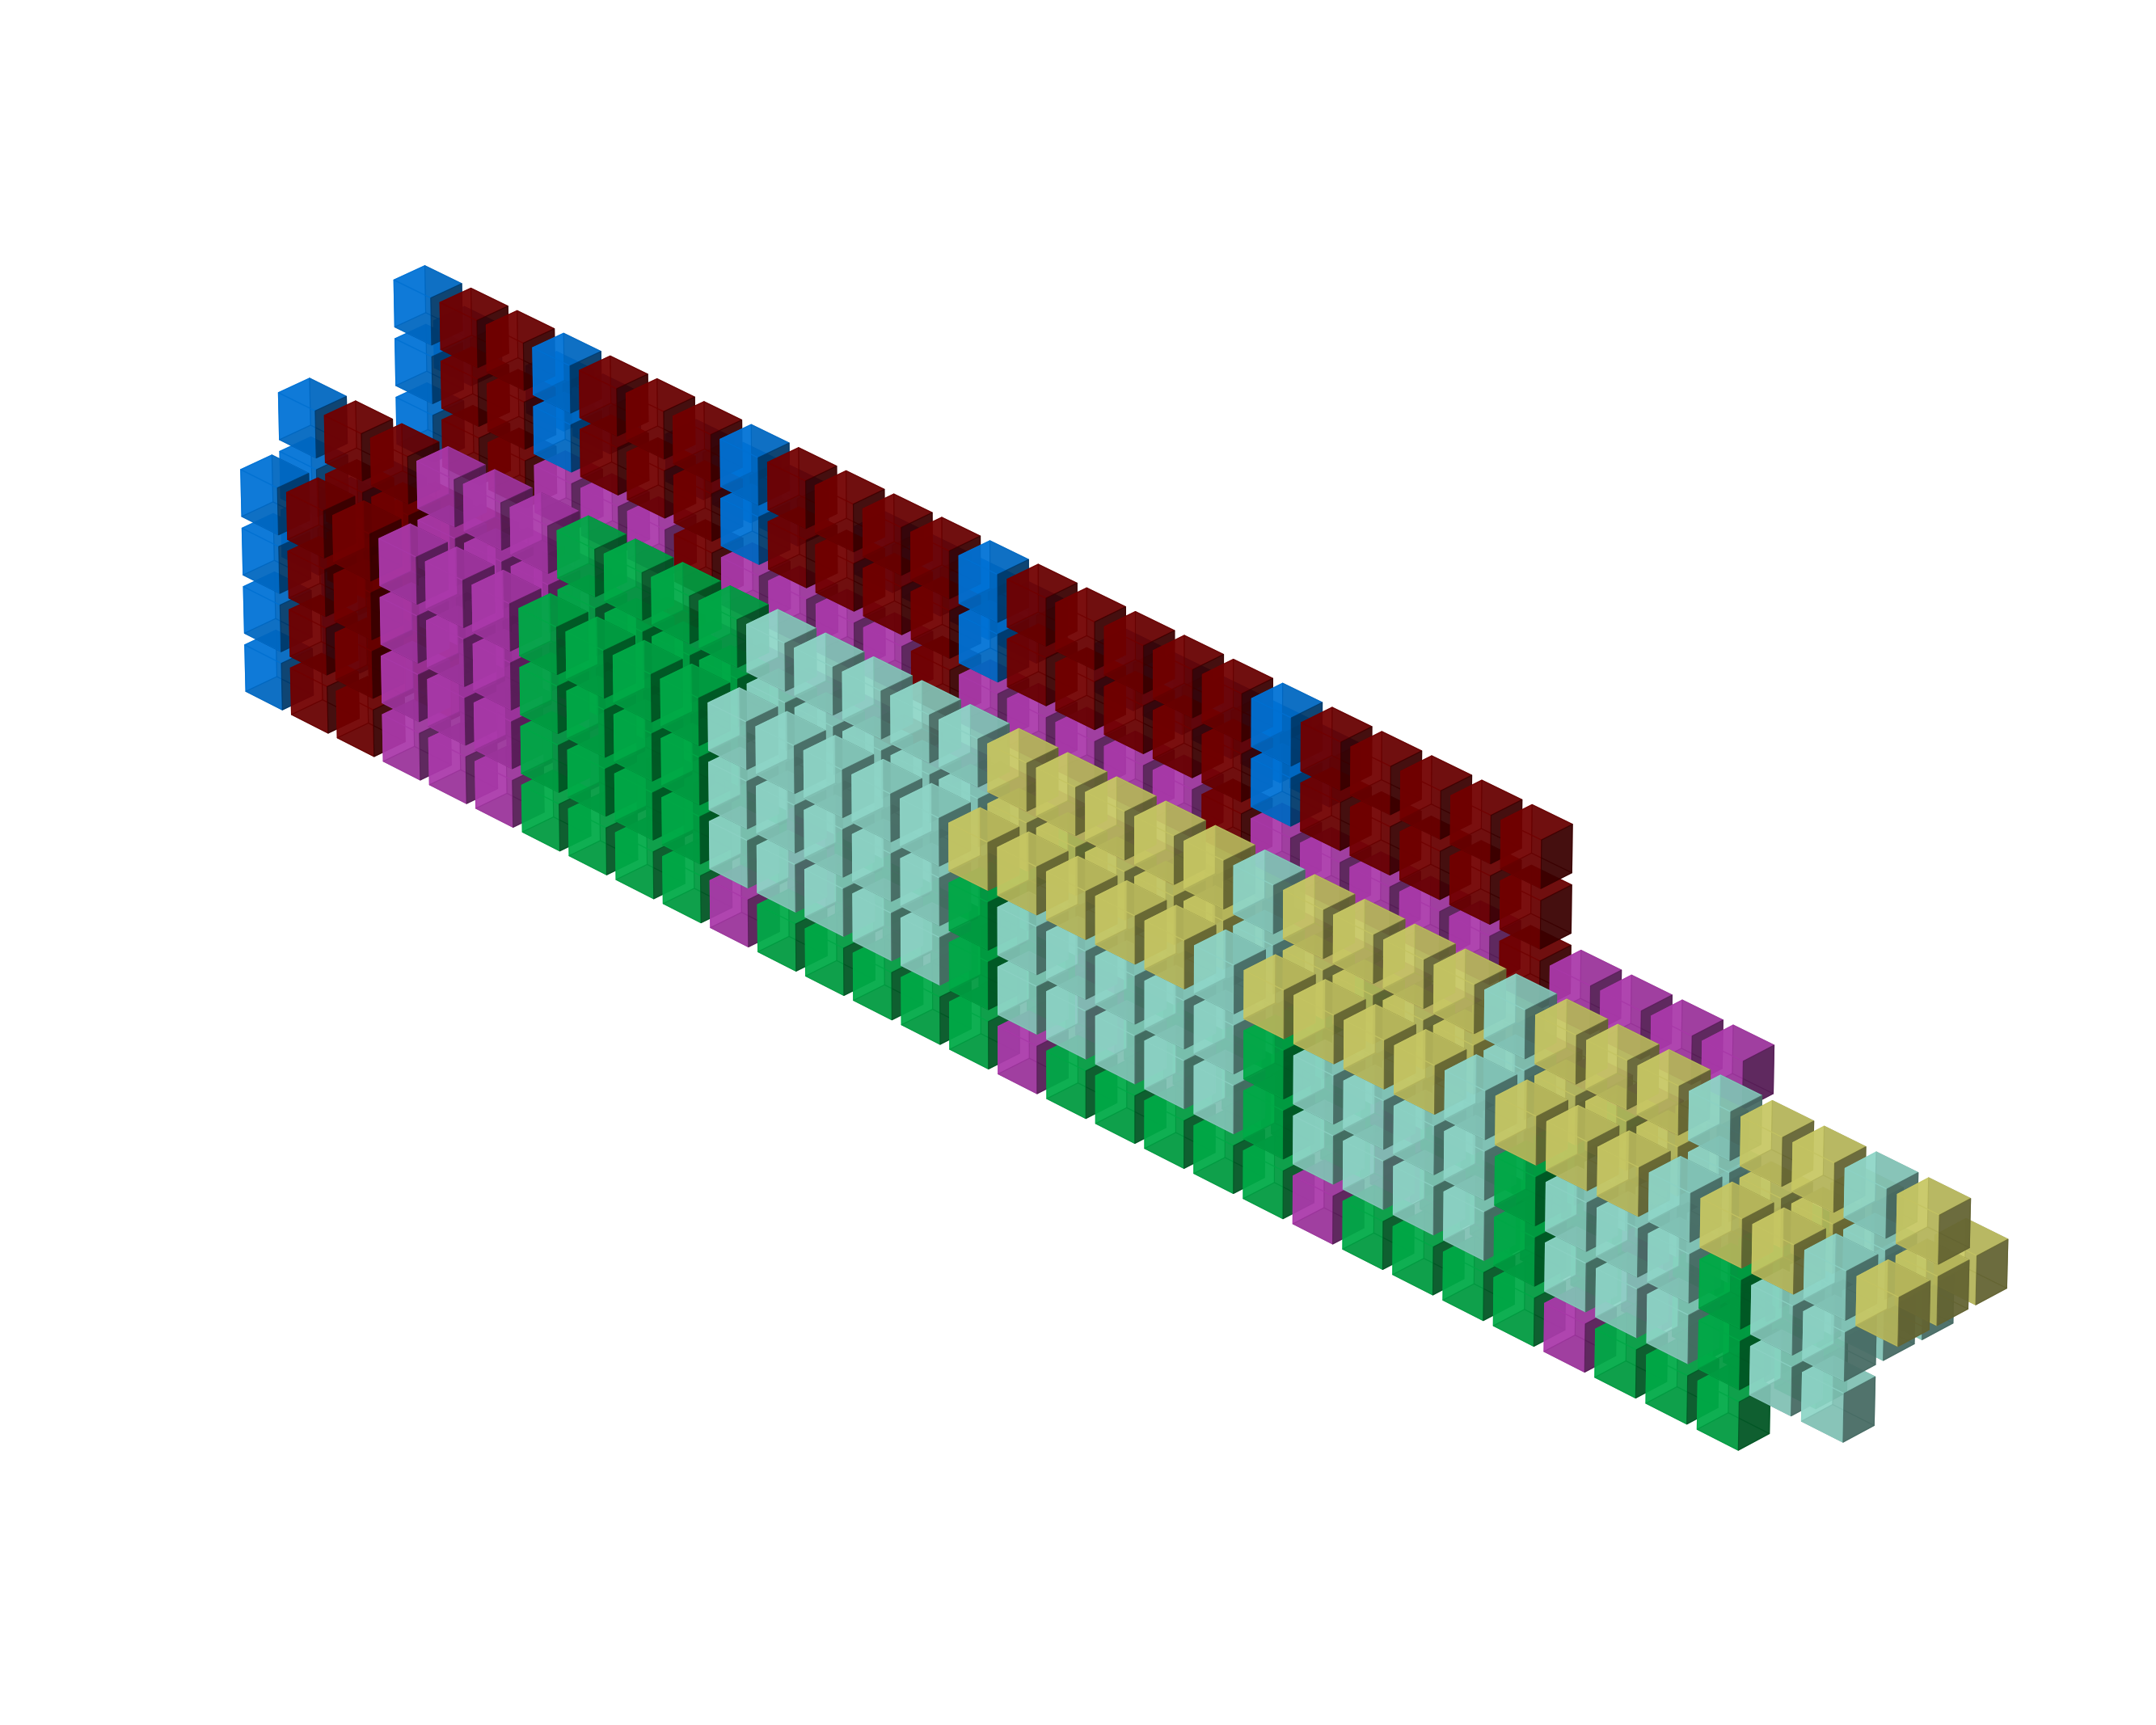
\includegraphics[width=12cm]{src/patterns/pattern11-225.png}%
    \end{adjustbox}
\caption{'Custom Pattern 4'.}
\end{figure}
\clearpage

\begin{lstlisting}
; customPattern3XPosArray             ;  5    
        .BYTE $00,$01,$01,$02,$55     ; 66  1 
        .BYTE $00,$00,$01,$02,$02,$55 ;  4 711
        .BYTE $00,$00,$00,$02,$55     ;   4222
        .BYTE $00,$FF,$FE,$55         ;    3 2
        .BYTE $00,$FE,$FE,$55         ;    3 3
        .BYTE $00,$FD,$FE,$55
        .BYTE $00,$55
; customPattern3YPosArray
        .BYTE $00,$FF,$00,$00,$55
        .BYTE $00,$01,$01,$01,$02,$55
        .BYTE $00,$02,$03,$03,$55
        .BYTE $00,$01,$00,$55
        .BYTE $00,$FF,$FE,$55
        .BYTE $00,$FF,$FF,$55
        .BYTE $00,$55
\end{lstlisting}
\subfile{patterns/tables/pattern11.tex}

\begin{figure}[H]
    \centering
    \begin{adjustbox}{width=12cm,center}
      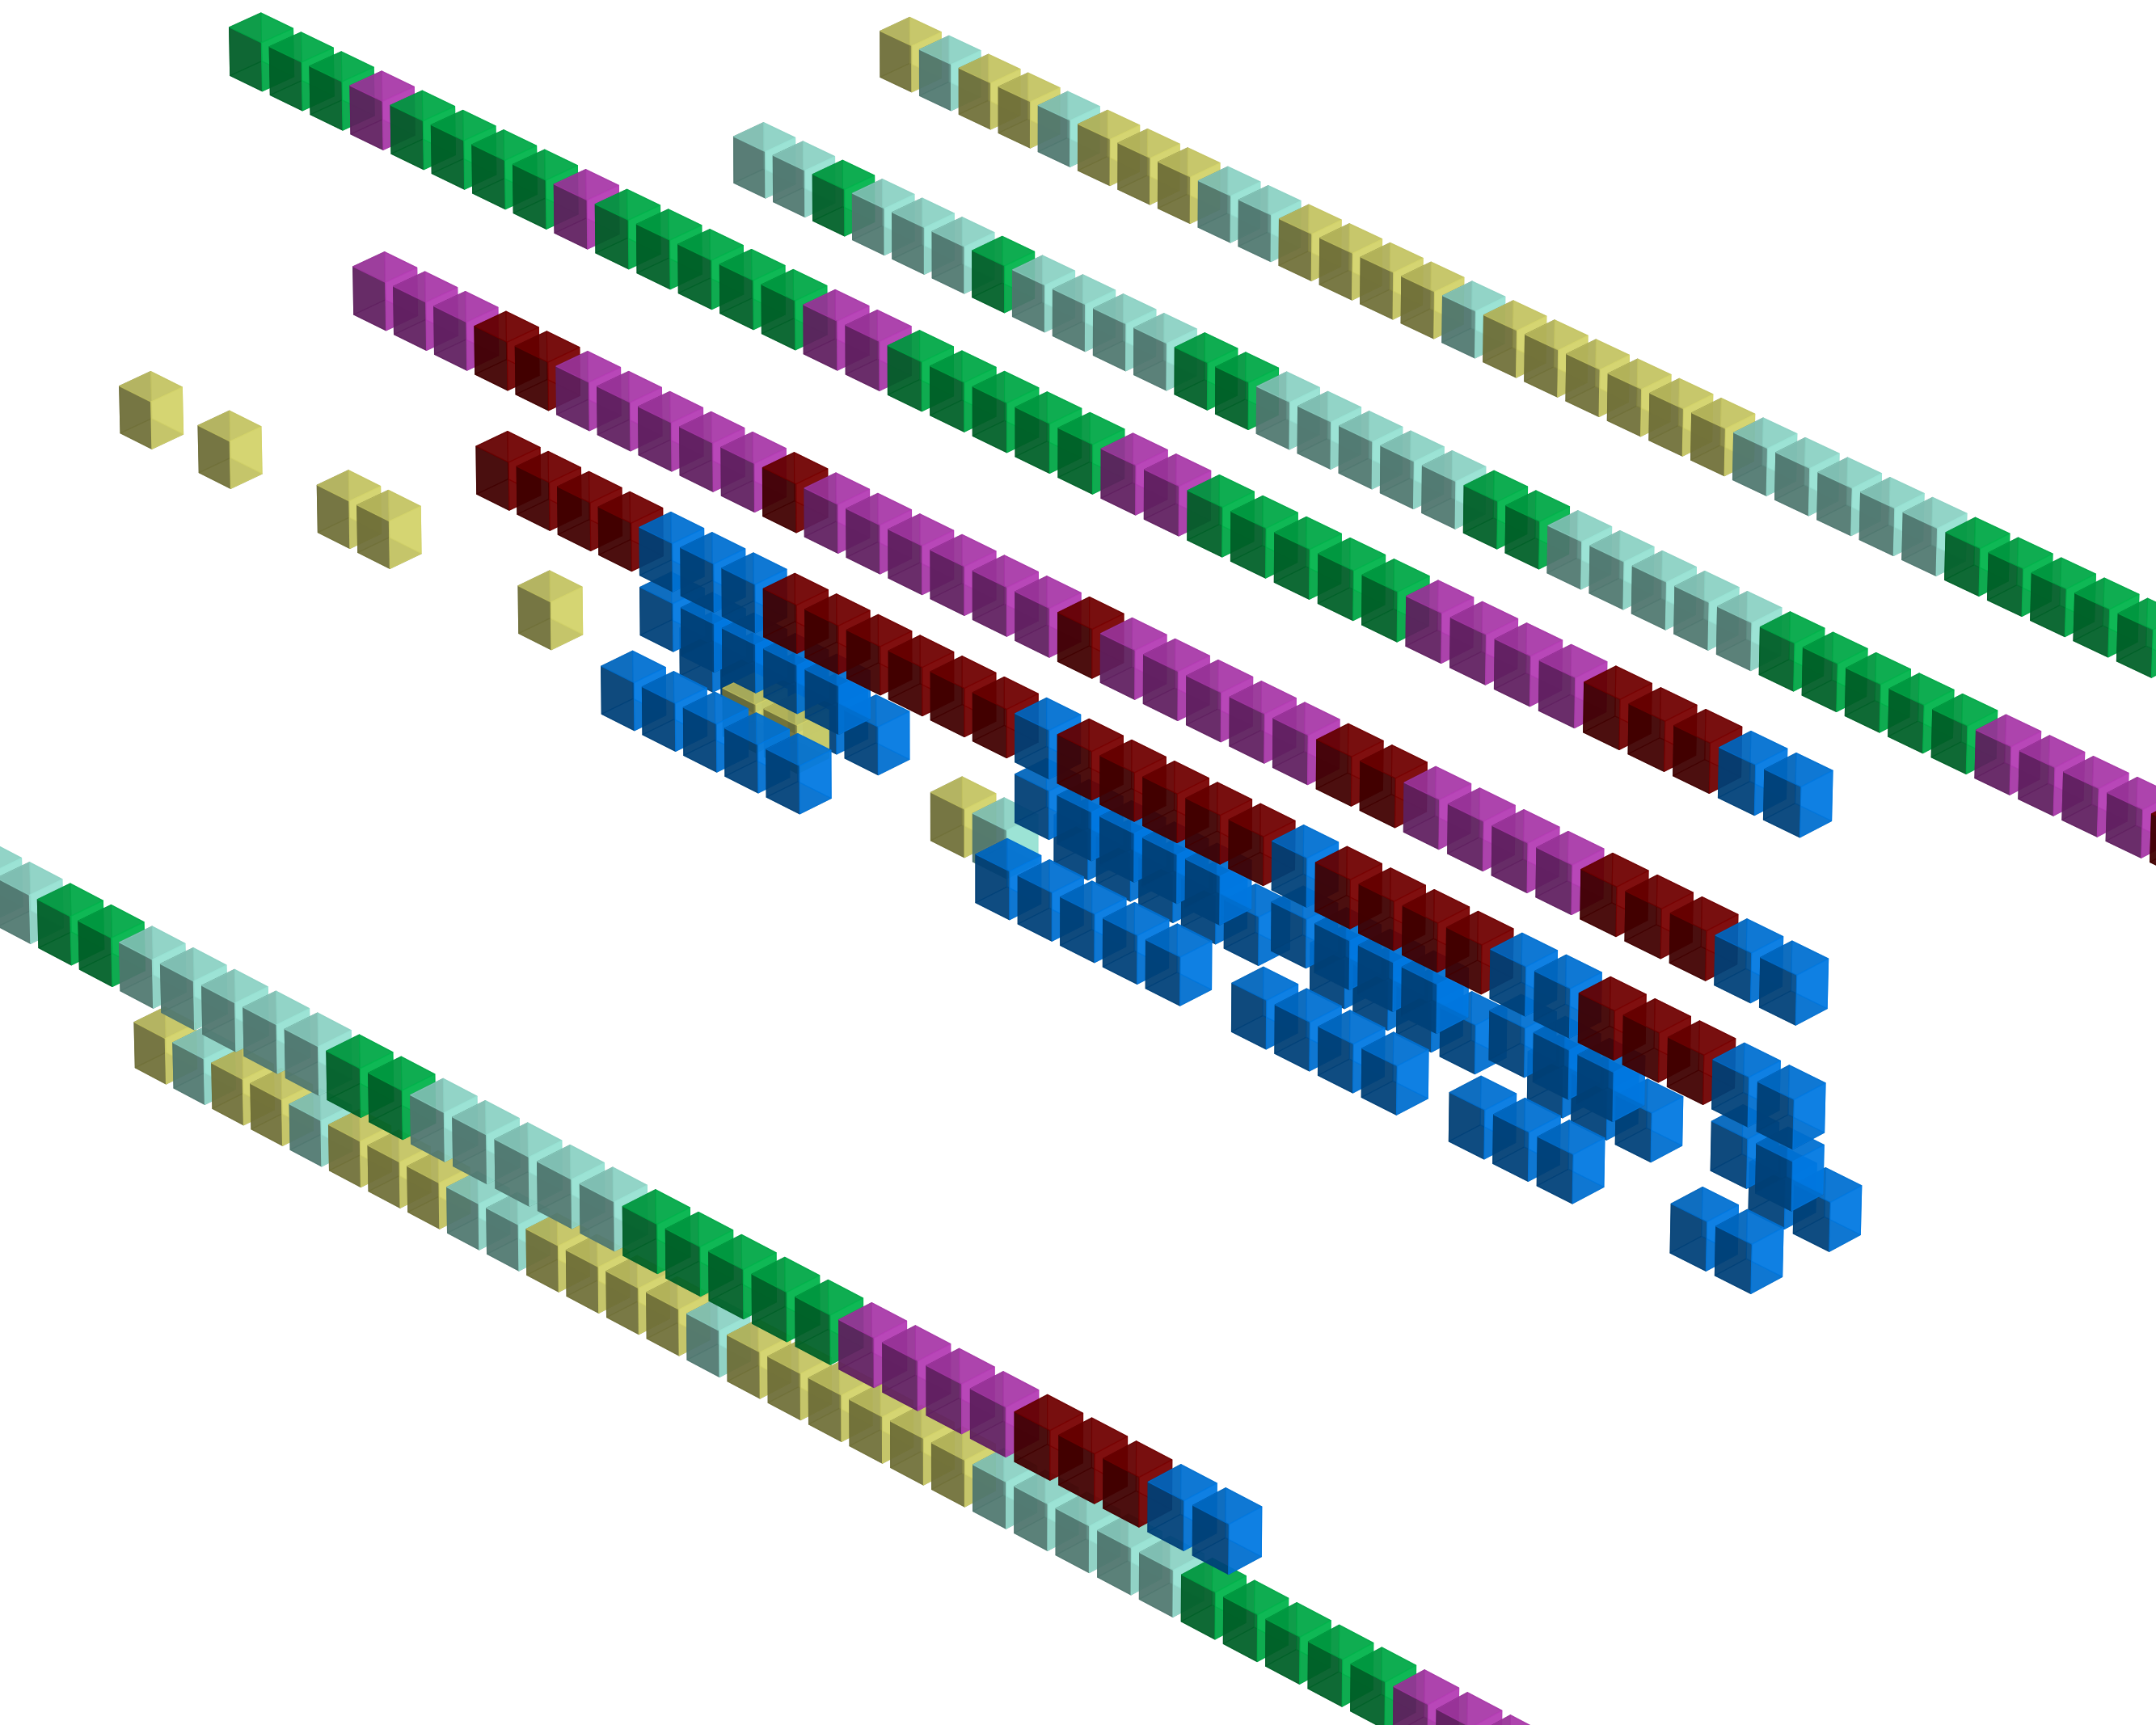
\includegraphics[width=12cm]{src/patterns/pattern12-45.png}%
    \end{adjustbox}
    \begin{adjustbox}{width=12cm,margin=0cm -4cm}
      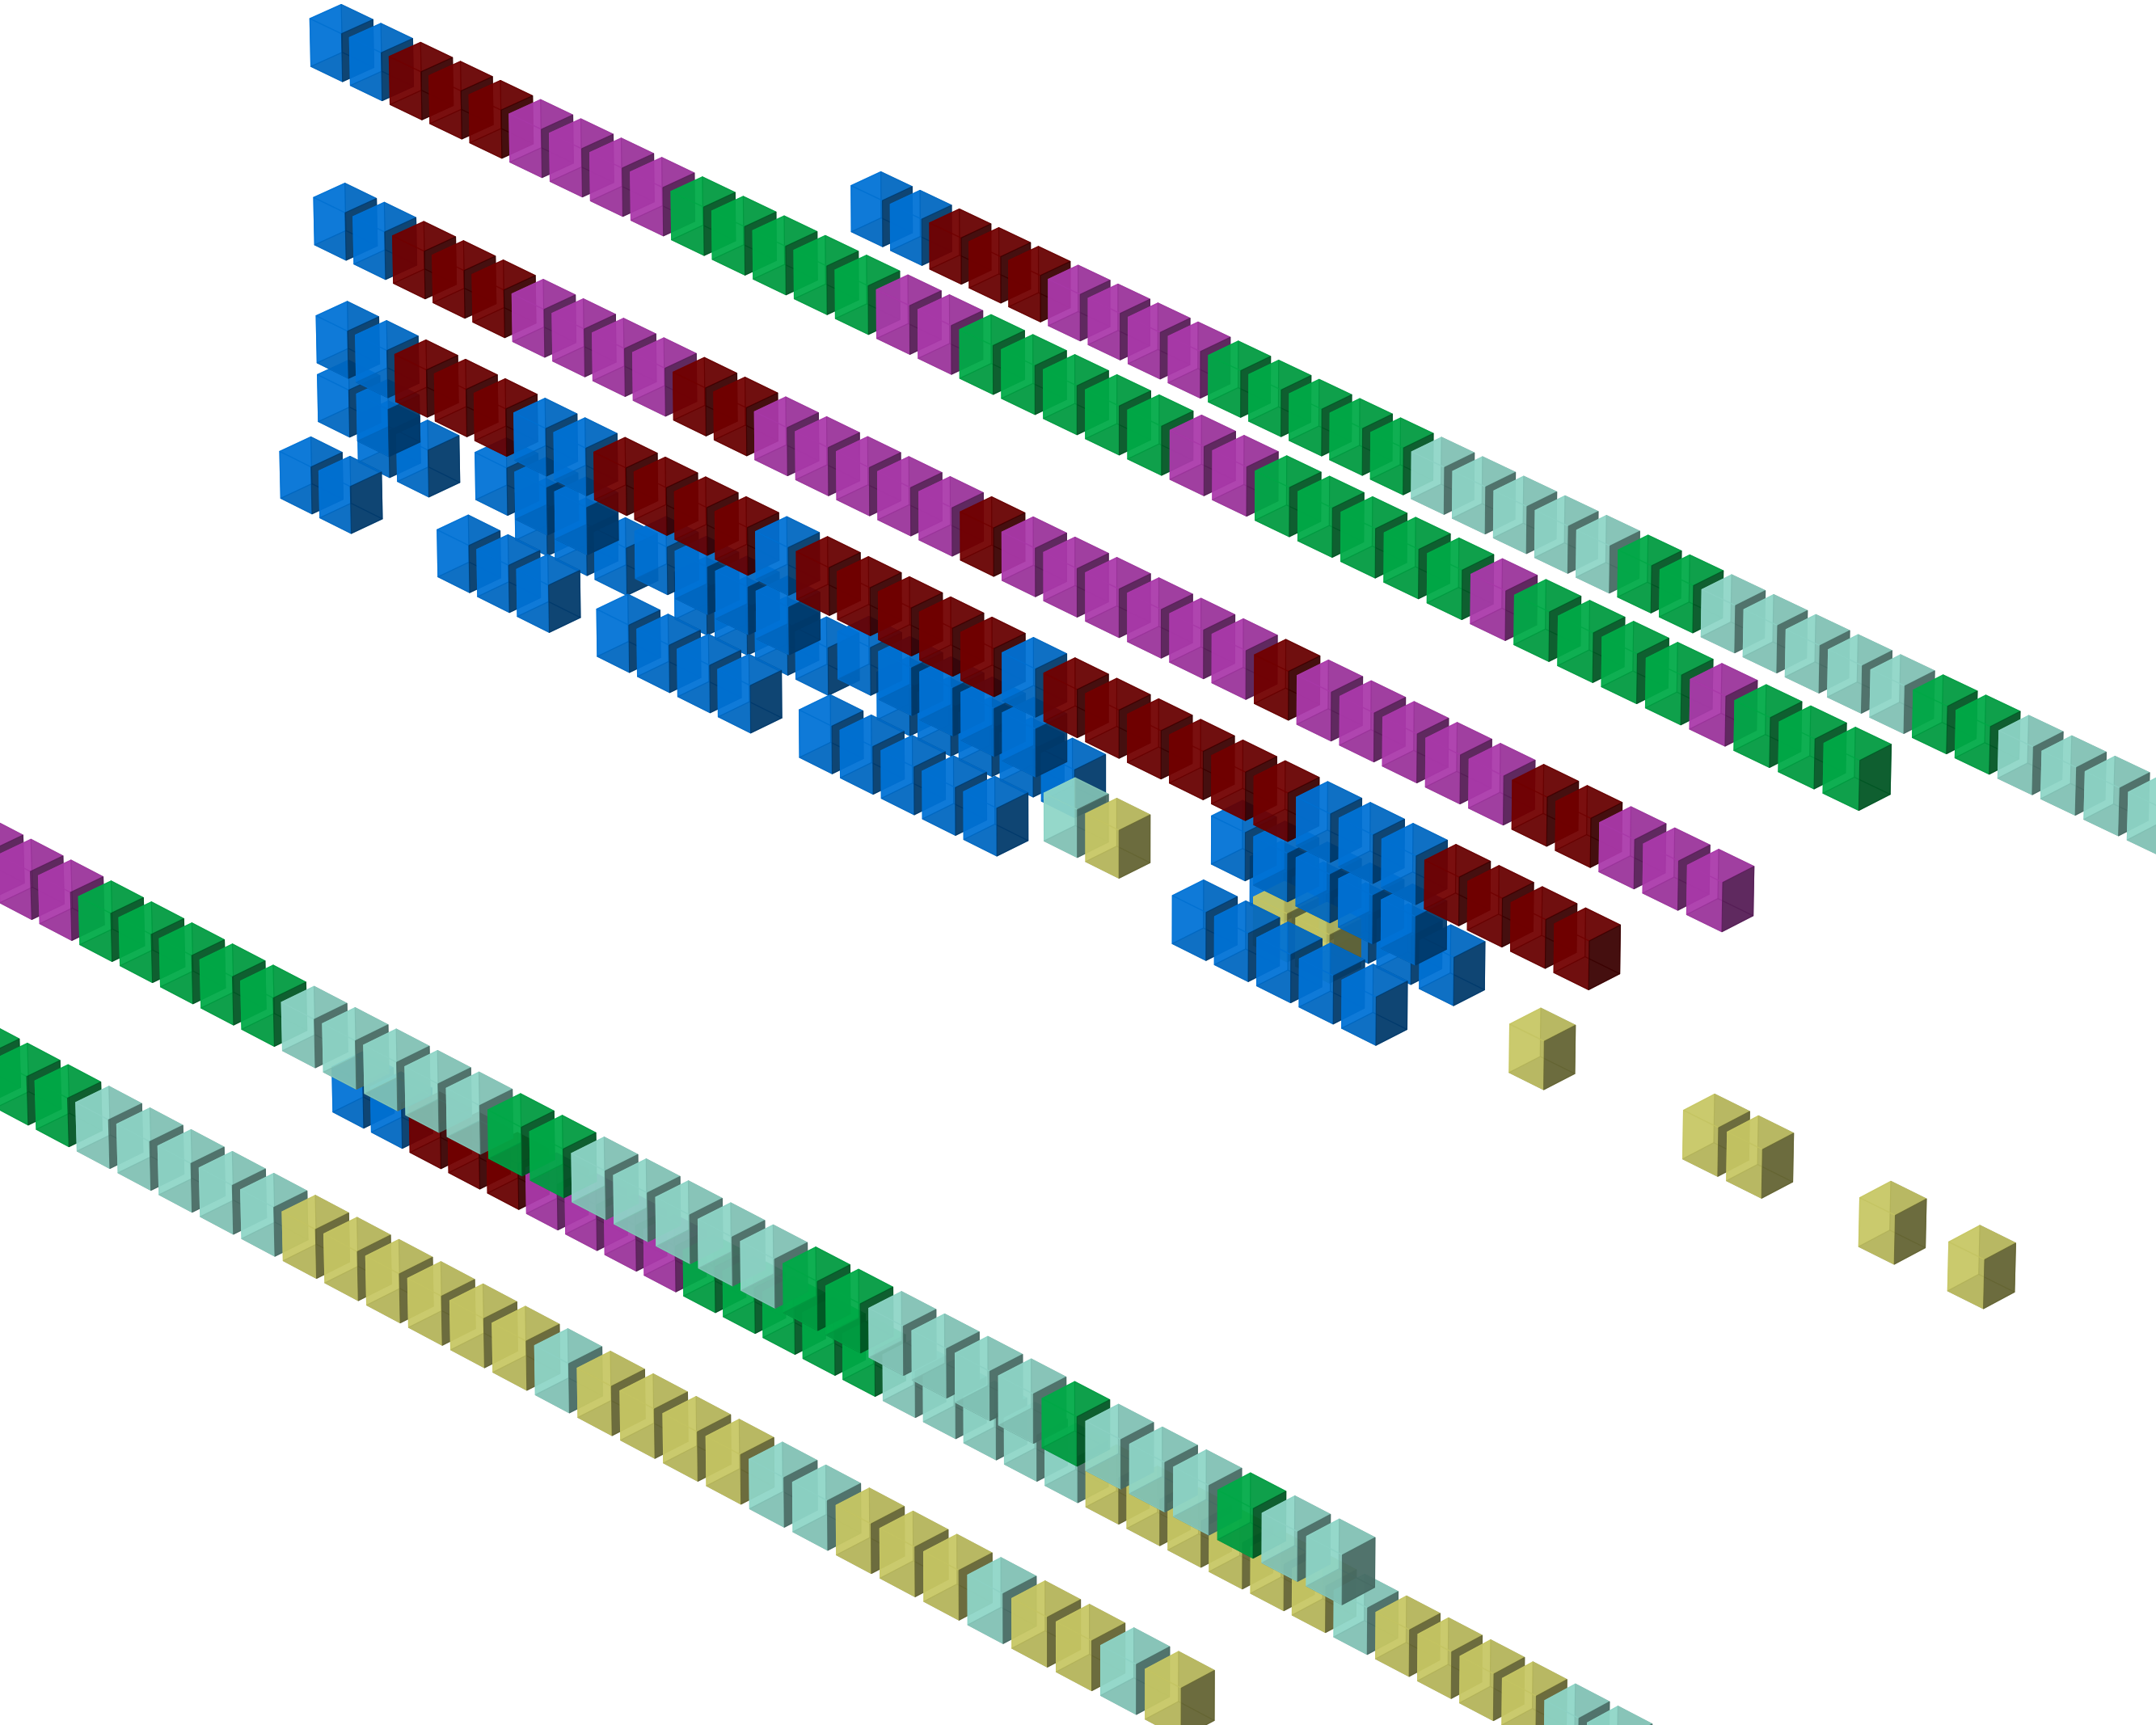
\includegraphics[width=12cm]{src/patterns/pattern12-225.png}%
    \end{adjustbox}
\caption{'Custom Pattern 5'.}
\end{figure}
\clearpage

\begin{lstlisting}[basicstyle=\tiny]
 ; customPattern4XPosArray      ;                 1                     
  .BYTE $00,$00,$00,$ED,$14,$55 ;                                       
  .BYTE $00,$F2,$0F,$55         ;                                       
  .BYTE $00,$00,$55             ;                                       
  .BYTE $00,$00,$55             ;                                       
  .BYTE $00,$00,$55             ;                 3                     
  .BYTE $00,$00,$FF,$01,$55     ;                                       
  .BYTE $00,$55                 ;                                       
  .BYTE $02,$55                 ;                 4                     
  .BYTE $00,$FC,$FD,$03,$04,$55 ;                                       
  .BYTE $00,$55                 ;                 5                     
                                ;                 6                     
; customPattern4YPosArray       ; 1    2      99 6106899      2    1    
  .BYTE $00,$0B,$F4,$00,$00,$55 ;                                       
  .BYTE $00,$00,$00,$55         ;                                       
  .BYTE $00,$F9,$55             ;                                       
  .BYTE $00,$FC,$55             ;                                       
  .BYTE $00,$FE,$55             ;                                       
  .BYTE $00,$FF,$00,$00,$55     ;                                       
  .BYTE $00,$55                 ;                                       
  .BYTE $00,$55                 ;                                       
  .BYTE $00,$00,$00,$00,$00,$55 ;                                       
  .BYTE $00,$55                 ;                                       
                                ;                 1                     
\end{lstlisting}
\subfile{patterns/tables/pattern12.tex}

\begin{figure}[H]
    \centering
    \begin{adjustbox}{width=12cm,center}
      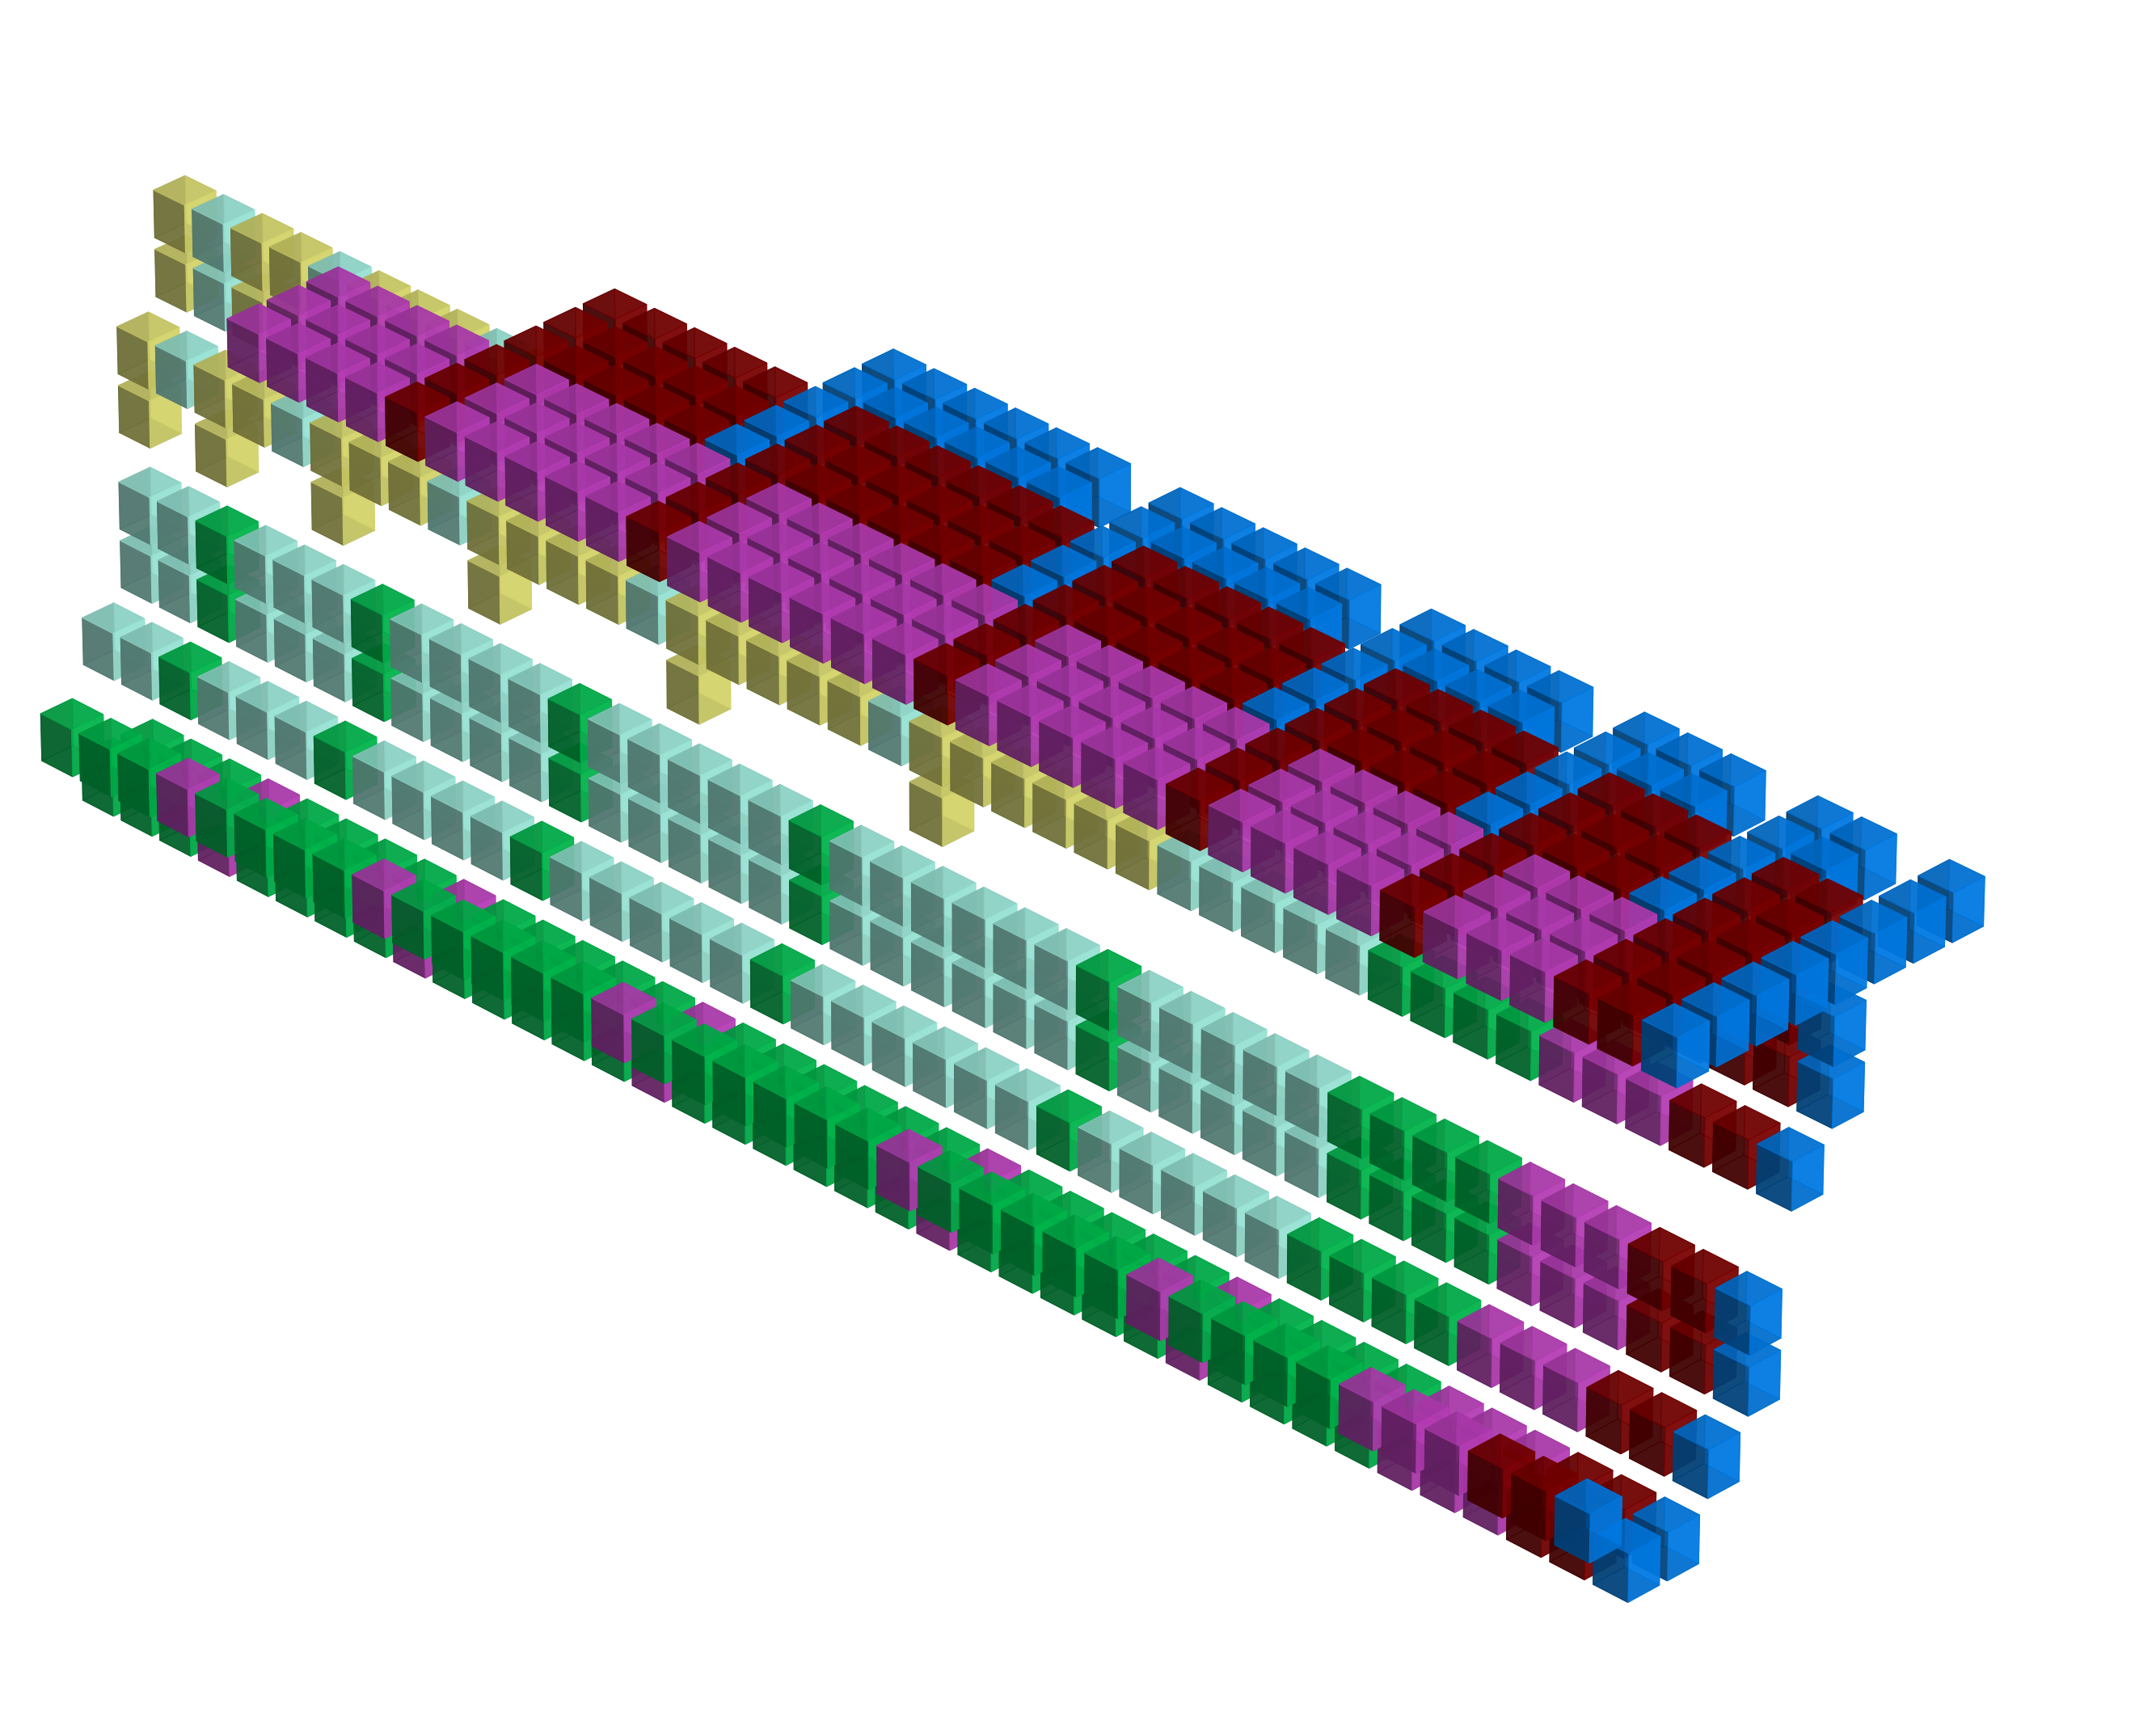
\includegraphics[width=12cm]{src/patterns/pattern13-45.png}%
    \end{adjustbox}
    \begin{adjustbox}{width=12cm,margin=0cm -4cm}
      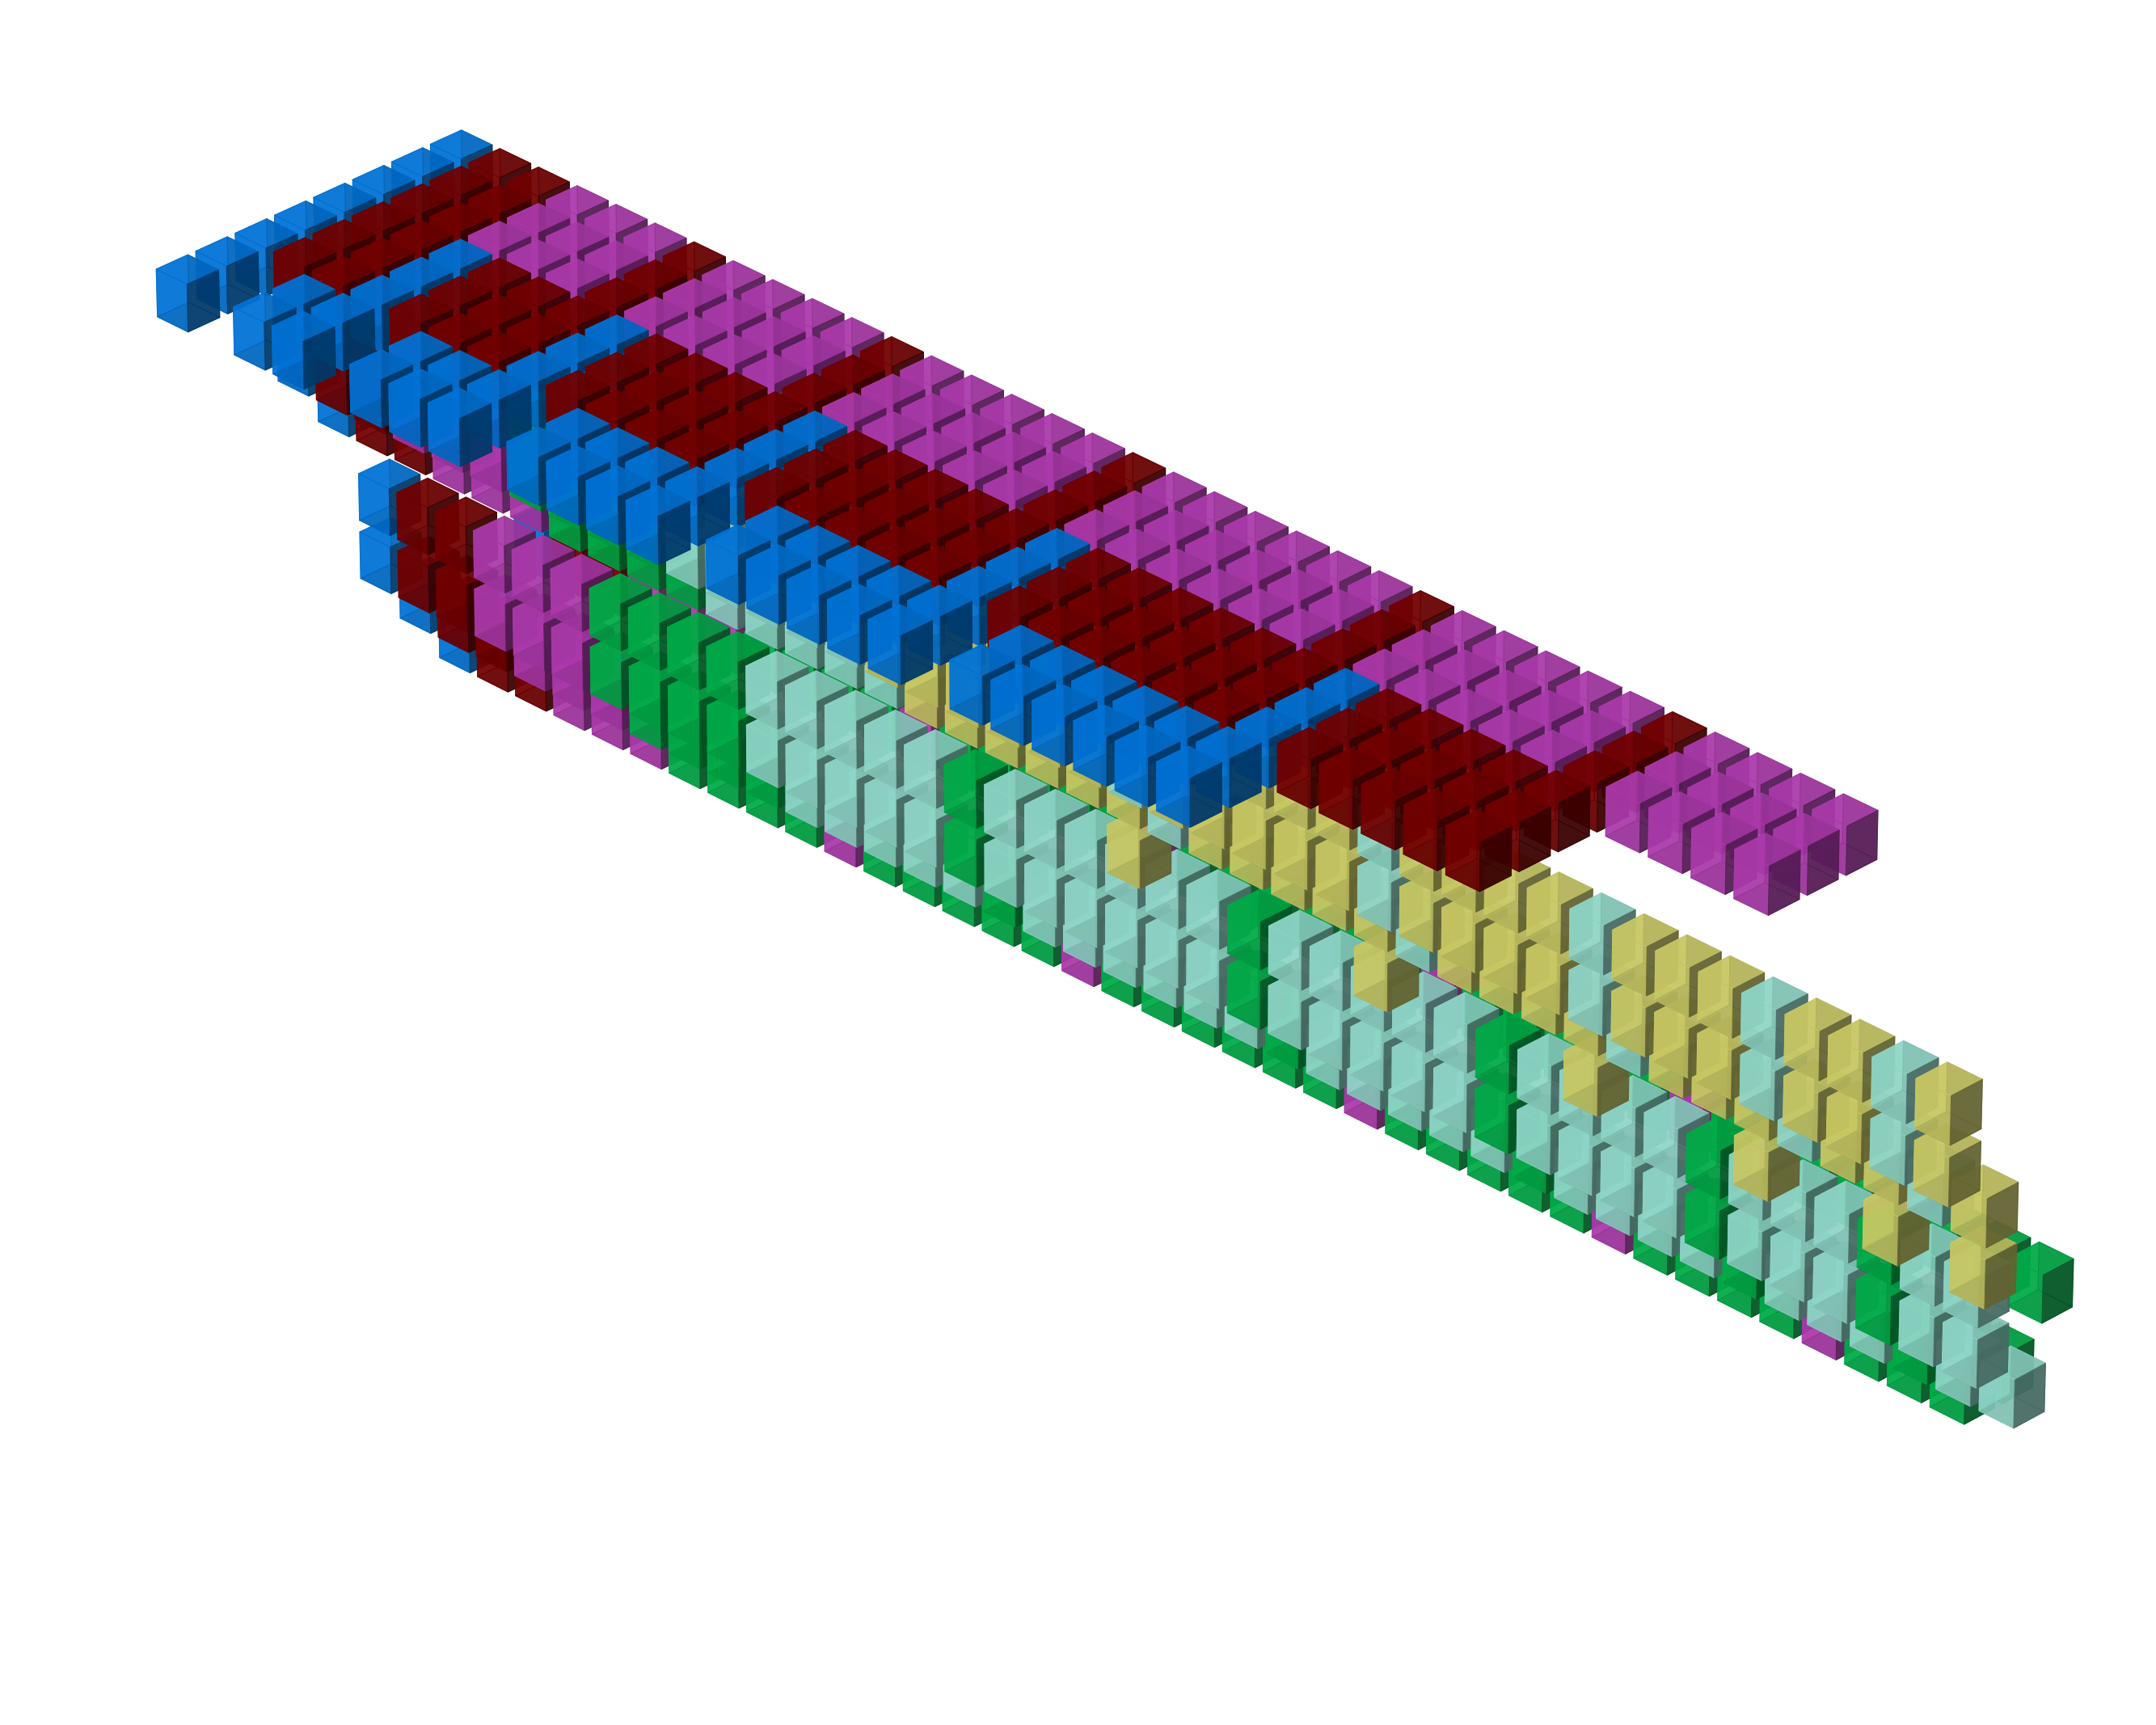
\includegraphics[width=12cm]{src/patterns/pattern13-225.png}%
    \end{adjustbox}
\caption{'Custom Pattern 6'.}
\end{figure}
\clearpage

\begin{lstlisting}
; customPattern5XPosArray          ;   44455566
        .BYTE $00,$00,$01,$01,$55  ;       1   
        .BYTE $00,$FF,$FF,$FE,$55  ;       1   
        .BYTE $00,$FD,$FC,$FB,$55  ;      1    
        .BYTE $00,$FD,$FE,$FF,$55  ;      7    
        .BYTE $00,$00,$01,$02,$55  ;     2     
        .BYTE $00,$03,$04,$55      ;     2     
        .BYTE $00,$55              ; 3  2      
                                   ;  33       
; customPattern5YPosArray
        .BYTE $00,$FF,$FE,$FD,$55
        .BYTE $00,$01,$02,$03,$55
        .BYTE $00,$04,$04,$03,$55
        .BYTE $00,$FC,$FC,$FC,$55
        .BYTE $00,$FC,$FC,$FC,$55
        .BYTE $00,$FC,$FC,$55
        .BYTE $00,$55
\end{lstlisting}
\subfile{patterns/tables/pattern13.tex}

\begin{figure}[H]
    \centering
    \begin{adjustbox}{width=12cm,center}
      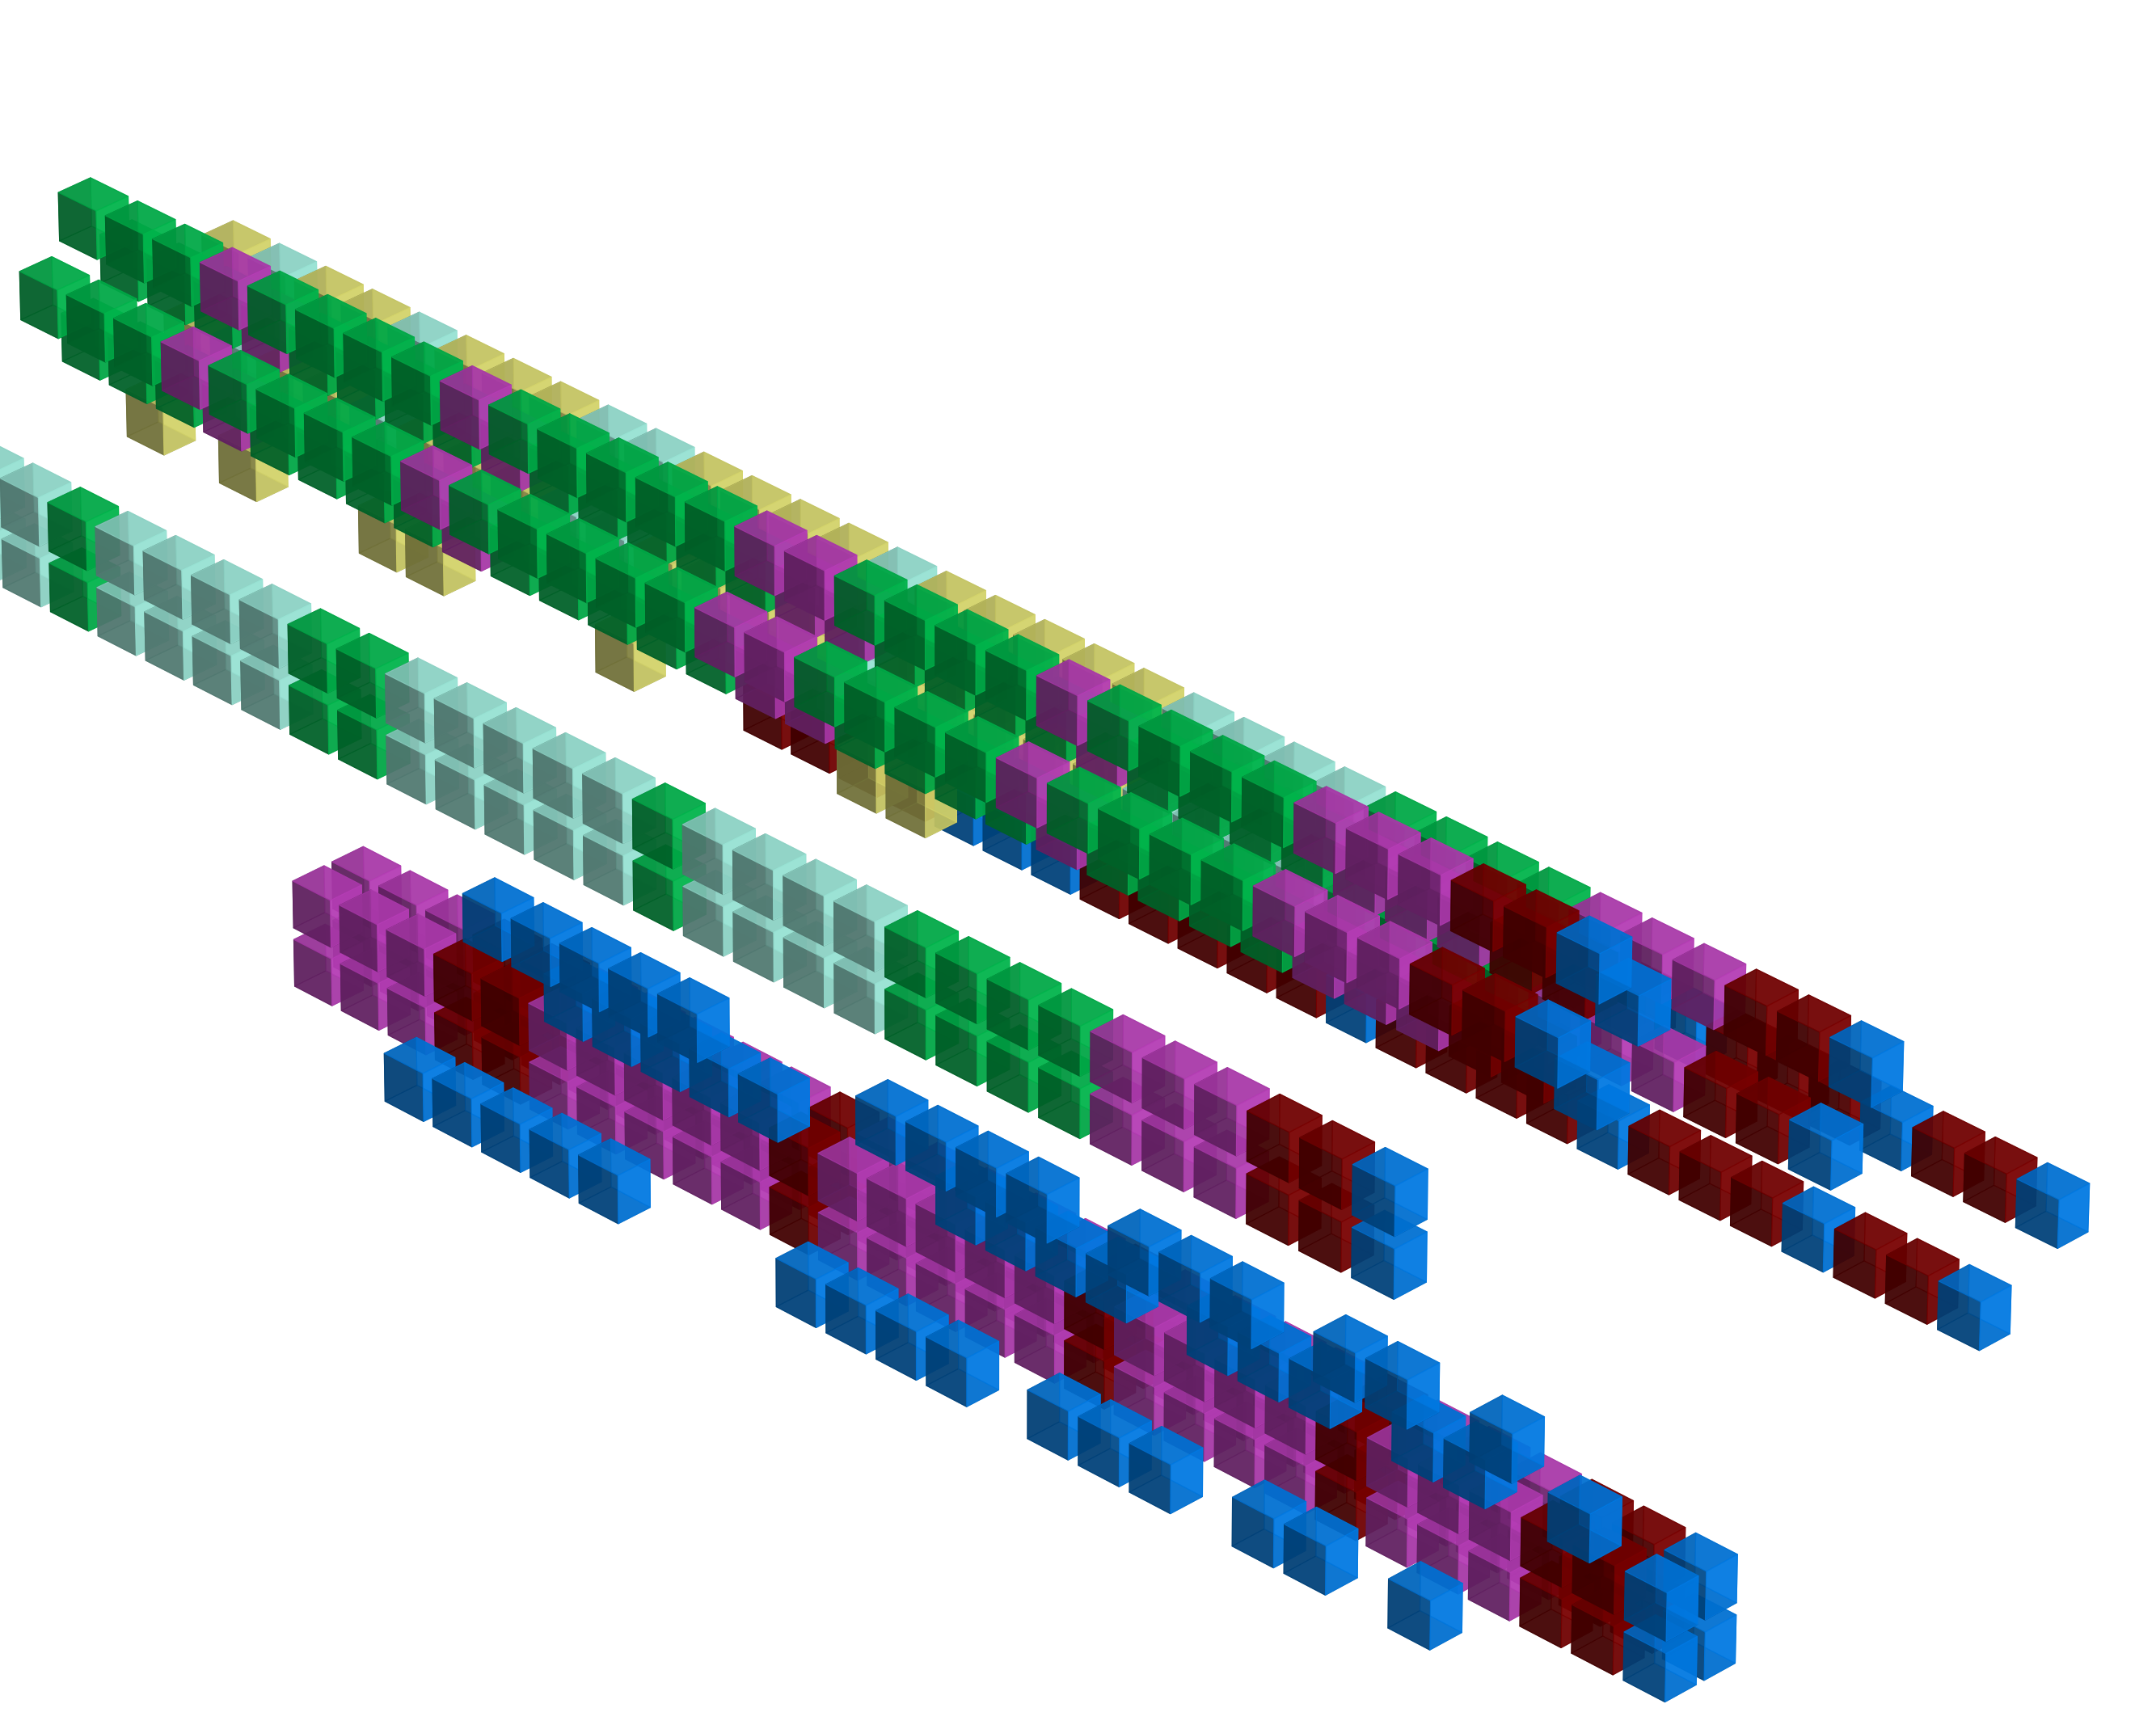
\includegraphics[width=12cm]{src/patterns/pattern14-45.png}%
    \end{adjustbox}
    \begin{adjustbox}{width=12cm,margin=0cm -4cm}
      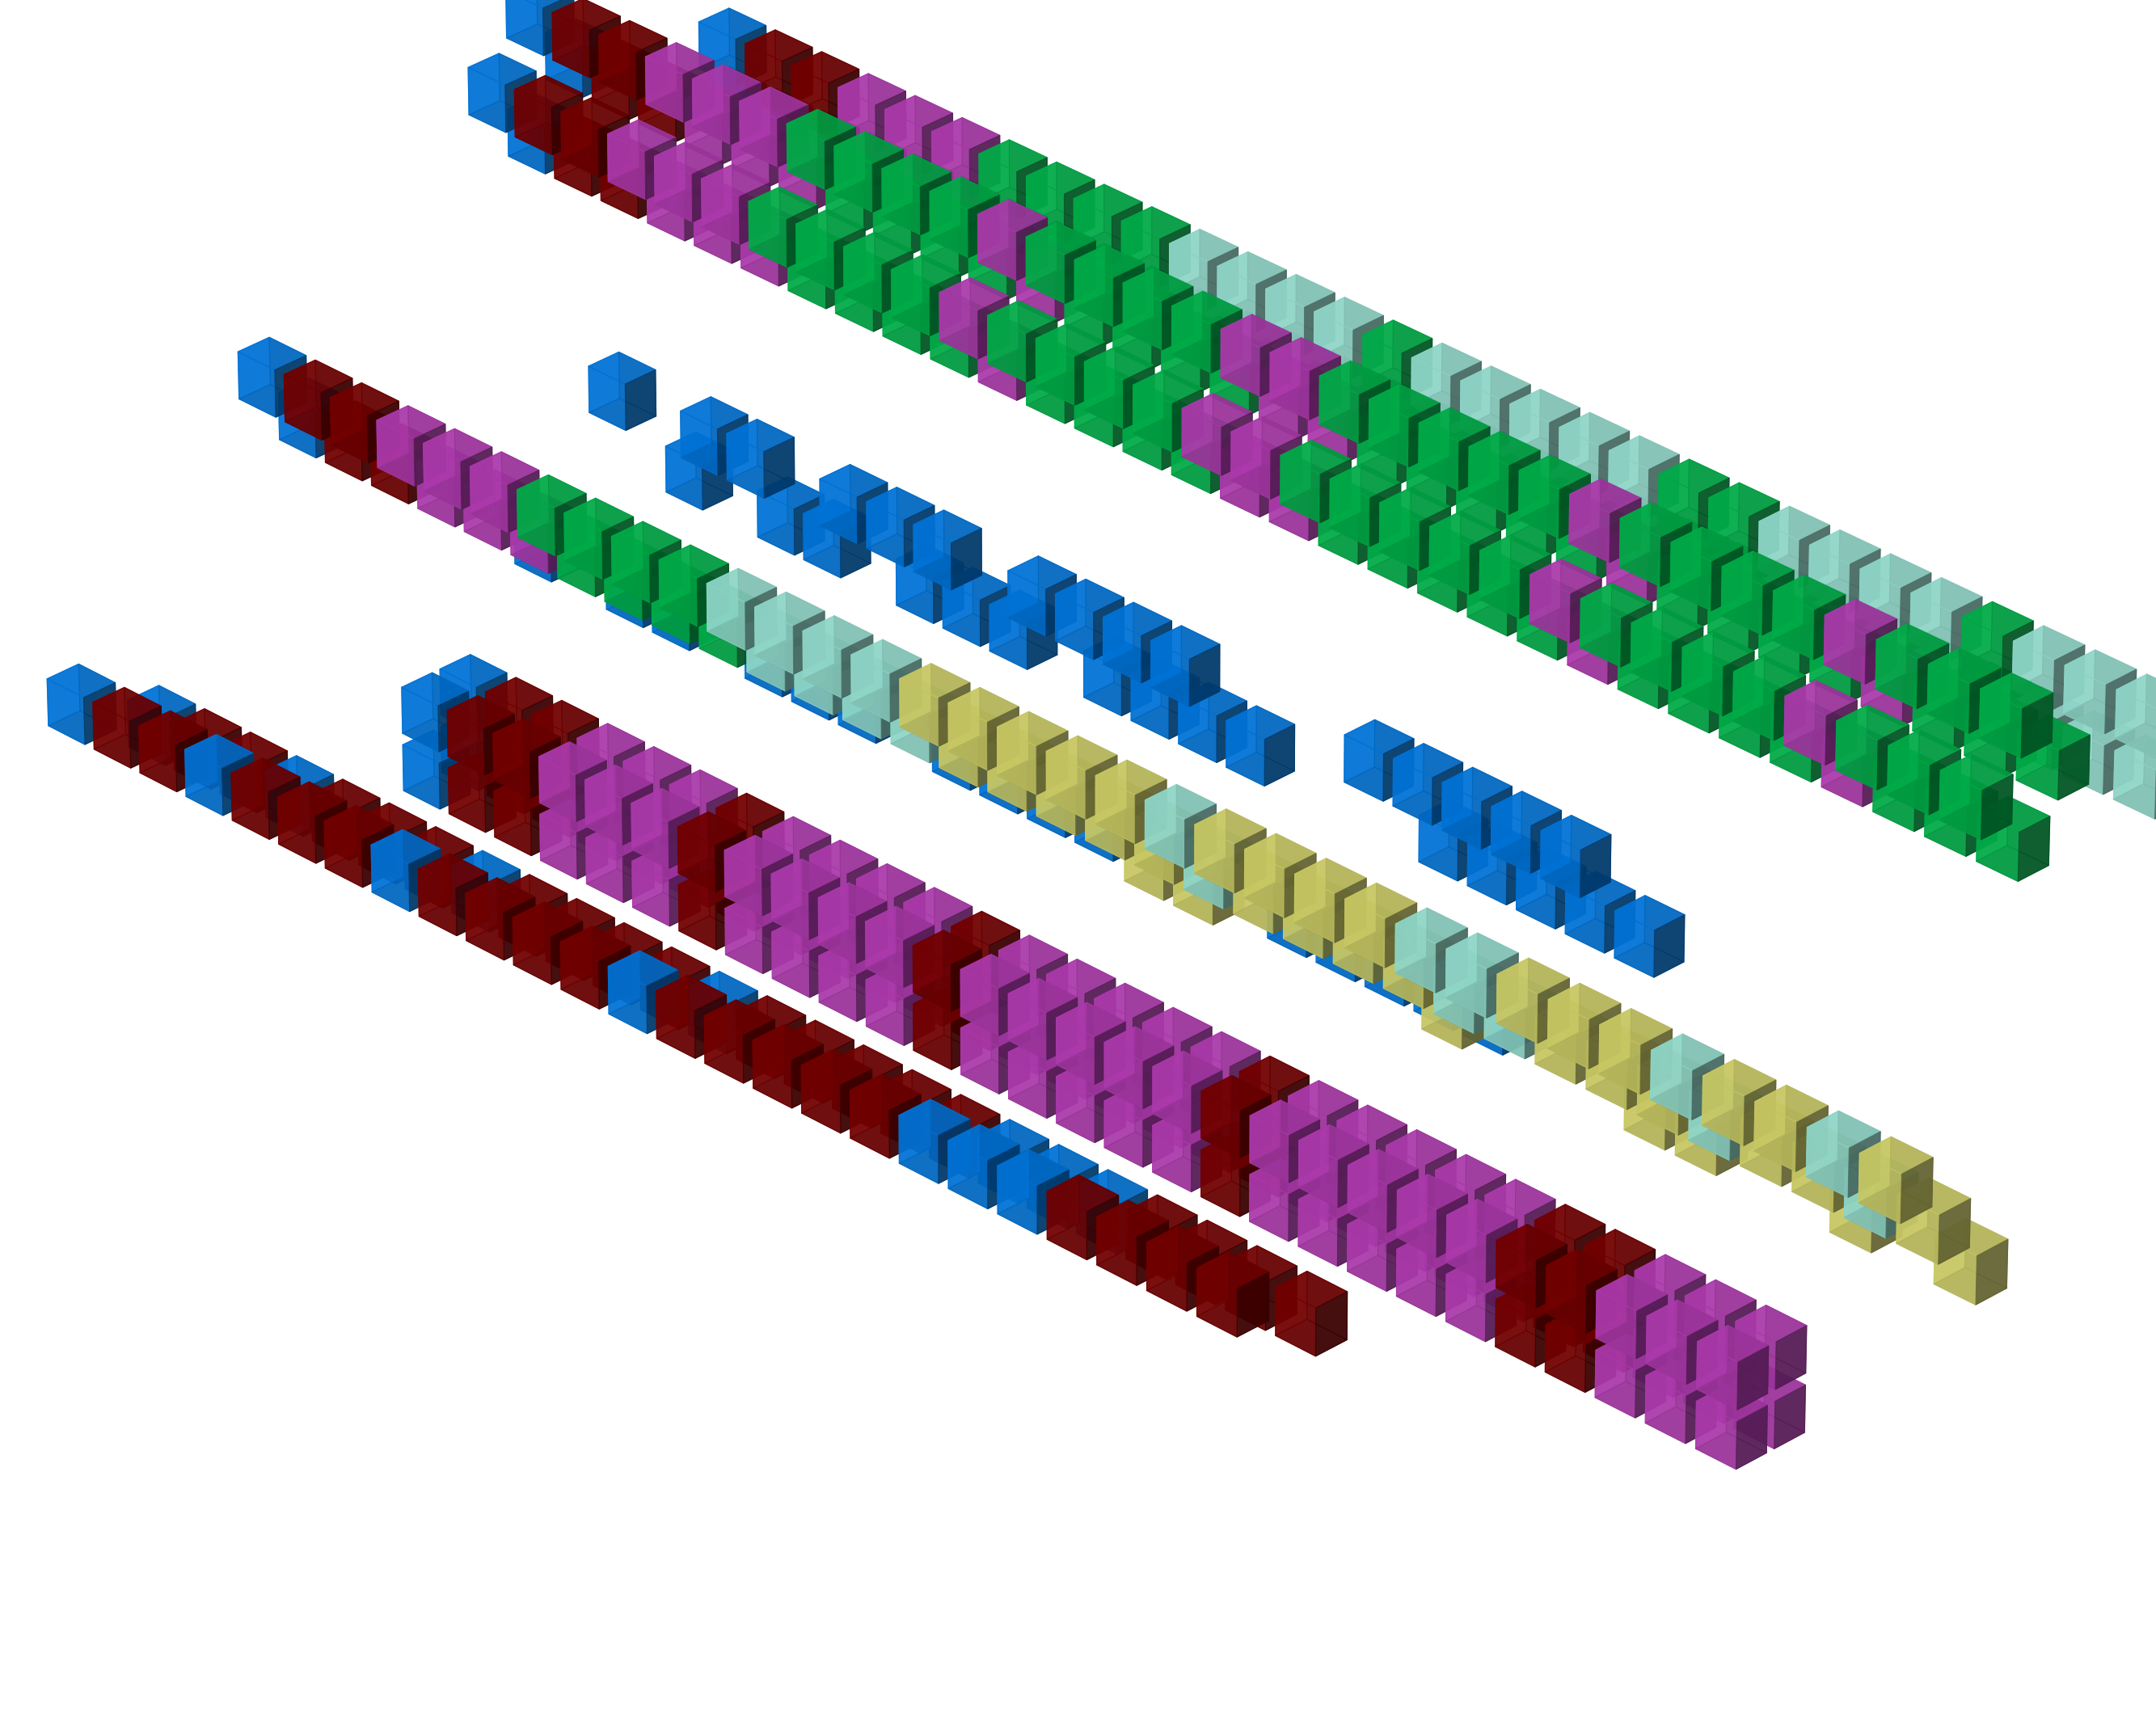
\includegraphics[width=12cm]{src/patterns/pattern14-225.png}%
    \end{adjustbox}
\caption{'Custom Pattern 7'.}
\end{figure}
\clearpage

\begin{lstlisting}
; customPattern6XPosArray             ;      3            
        .BYTE $00,$01,$02,$55         ;     3 3           
        .BYTE $00,$F6,$F6,$55         ; 2    3            
        .BYTE $00,$FB,$FA,$FB,$FC,$55 ; 2                 
        .BYTE $00,$FD,$FD,$FE,$FE,$55 ;             1     
        .BYTE $00,$05,$07,$55         ;            1      
        .BYTE $00,$F9,$F7,$FB,$55     ;           8       
        .BYTE $00,$55                 ;    6              
        .BYTE $00,$55                 ;                  5
                                      ;  6   6         5  
; customPattern6YPosArray             ;                   
        .BYTE $00,$FF,$FE,$55         ;        44         
        .BYTE $00,$FC,$FD,$55         ;        44         
        .BYTE $00,$FA,$FB,$FC,$FB,$55
        .BYTE $00,$05,$06,$06,$05,$55
        .BYTE $00,$03,$02,$55
        .BYTE $00,$01,$03,$03,$55
        .BYTE $00,$55
        .BYTE $00,$55
\end{lstlisting}
\subfile{patterns/tables/pattern14.tex}

